\documentclass[letterpaper,12pt]{report}
\usepackage{palatino,url,graphicx}
\usepackage[utf8]{inputenc}
\usepackage{amsmath}
\usepackage{setspace}
\usepackage{appendix}
\usepackage[graph, frame]{xy} % For X-MIMI prbac Chapter
\usepackage[final]{pdfpages}
\usepackage{listings}
\usepackage{pgf,tikz}
\usetikzlibrary{shapes,arrows,snakes,automata,backgrounds,trees,calc,matrix,positioning,fit}
\usepackage{colortbl}
\usepackage{enumerate}
%\usepackage[lined,boxed,linesnumbered]{algorithm2e}
%\usepackage{algorithmic}
\usepackage{boxedminipage}
\usepackage{multirow}
\usepackage{url}
\usepackage[font={small,it}]{caption}
\usepackage{rotating}
\usepackage{array}
\usepackage{pdflscape}
\usepackage{bm}
\usepackage{pdfpages}
\usepackage{moreverb}
\usepackage{algpseudocode}
\usepackage{algorithm}
\usepackage[utf8]{inputenc}
\usepackage[T1]{fontenc}


\lstset{
	%language=ruby,
	keywordstyle=\bfseries\ttfamily\color[rgb]{0,0,1},
	identifierstyle=\ttfamily,
	commentstyle=\color[rgb]{0.133,0.545,0.133},
	stringstyle=\ttfamily\color[rgb]{0.627,0.126,0.941},
	showstringspaces=false,
	basicstyle=\small,
	numberstyle=\footnotesize,
	numbers=none,
	stepnumber=1,
	numbersep=10pt,
	tabsize=2,
	breaklines=true,
	prebreak = \raisebox{0ex}[0ex][0ex]{\ensuremath{\hookleftarrow}},
	breakatwhitespace=false,
	aboveskip={1.5\baselineskip},
  columns=fixed,
  extendedchars=true,
% frame=single,
% backgroundcolor=\color{lbcolor},
}

% http://www.tug.org/applications/hyperref/manual.html
\usepackage[breaklinks=true]{hyperref}
\hypersetup{
   bookmarks=false,         % show bookmarks bar?
%    unicode=false,          % non-Latin characters in Acrobat‚ bookmarks
%    pdftoolbar=true,        % show Acrobat‚ toolbar?
%    pdfmenubar=true,        % show Acrobat‚ menu?
%    pdffitwindow=false,     % window fit to page when opened
%    pdfstartview={FitH},    % fits the width of the page to the window
   pdftitle={Zhuofu dissertation},    % title
   pdfauthor={Zhuofu Bai},     % author
   pdfsubject={Ph.D. Dissertation},   % subject of the document
   % pdfcreator={TextMate},   % creator of the documentt
%    pdfproducer={Producer}, % producer of the document
%    pdfkeywords={keywords}, % list of keywords
%    pdfnewwindow=true,      % links in new window
   colorlinks=true,       % false: boxed links; true: colored links
   linkcolor=black,          % color of internal links
   citecolor=black,        % color of links to bibliography
   filecolor=black,      % color of file links
   urlcolor=black           % color of external links
}


\input xy
\xyoption{all}

\doublespacing

\setlength\oddsidemargin{0.5in}
\setlength\textwidth{6.0in}
\setlength\topmargin{0in}
\setlength\headheight{0in}
\setlength\headsep{0in}
\setlength\textheight{9in}
%%sets the textwidth to 6.5, which leaves 1 for the remaining right margin with 8 1/2X11inch paper


\begin{document}
  \pagenumbering{roman}

% UNCOMMENT BELOW
\title{LOCALIZING FAULTS IN NUMERICAL SOFTWARE USING A VALUE-BASED CAUSAL MODEL}
\author {by\\ZHUOFU BAI}
\date{\vspace{0.8cm}Submitted in partial fulfillment of the requirements\\
For the degree of Doctor of Philosophy\\
\vspace{0.45in}
Dissertation Advisor: Dr. Andy Podgurski\\
\vspace{0.45in}
Department of Electrical Engineering and Computer Science\\
CASE WESTERN RESERVE UNIVERSITY\\
\vspace{0.45in}
TBD}

\maketitle

% Committee Signature sheet (typed version)-originals turned in with Final Materials
% \includepdf{signature_sheet_filled_in.pdf}

% % Copyright page (only if copyrighting)
% \newpage
% Copyright page (only if copyrighting)

% % Dedication page (optional)
% \newpage
% Dedication page (optional)

% \singlespacing
%% UNCOMMENT BELOW
\setcounter{page}{3}
\tableofcontents
\listoftables
\listoffigures

% \doublespacing
%% UNCOMMENT BELOW
% % Preface (optional)
% \newpage
% Preface (optional)
% Acknowledgements (optional)

\newpage
\section*{Acknowledgements}
First and foremost, I would like to thank my advisor, Dr. Andy Podgurski for his constant support and guidance.  Dr. Podgurski led me into the field of software testing and reliability and guided me in every project. He is  knowledgable, responsible and patient.  Especially in the first few years of my PhD, I was stuck on my research and almost give up. Dr Podgurski shared his innovative ideas with me, and contributed a lot of time to help overcome the difficulties in my research. Everything would be different without him. 

My sincere thanks also go the members of my committee, Dr. Soumya Ray,  Dr. M. Cenk Cavusoglu and Dr. Xiang Zhang for their invaluable feedback, scientific suggestions and insightful discussions, which helped me improve this dissertation. I would like to give special thanks to Dr. Soumya Ray, who generously offered advices and shared research experiences with me during my Ph.D. study.

I would like to thank all my co-workers at Case Western Reserve University: Dr. Boya Sun, Dr. Gang Shu, Shih-feng Sun, Dr. Mark Renfrew, Feng Cao, Kai Liang,  Erdem Tuna. This work will be impossible without their support and cooperation. I am thankful to my close friends, Jiangli Zhu, Yang Zhang, Jiale Li, Xuefei Wang. 

I deeply appreciate my parents, Xiaomin Wang and Baodong Bai, for their unconditional love and support. My wife, Yang Chen, always encourage me and gives me her best possible support. Thank you, Yang. I couldn’t have done it without you. 



% List of Abbreviations (optional)
\newpage
\section*{List of Abbreviations}
\begin{itemize}
  \item OMIM: Online \lowercase{Mendelian Inheritance in Man}
  \item GWAS: Genome-wide association study
  \item UMLS: Unified \lowercase{Medical Language System}
  \item CBIR: Content-based image retrieval
  \item SIFT: Scale invariant feature transformation
  \item HOG: Histograms of oriented gradients
  \item SVM: support vector machine
  \item HPRD: Human \lowercase{Protein Reference Database}
  \item PPI: Protein-protein interaction
  \item HDN: Human disease network
  \item CRC: Colorectal cancer
  \item PD: Parkinson's disease
  \item DMN: Disease manifestation network
  \item IMPC: International \lowercase{Mouse Phenotyping Consortium}
  \item FDA: Food and drug administration

\end{itemize}

\newpage
\begin{centering}
  Localizing Faults in Numerical Software Using a Value-Based Causal Model
  LOCALIZING FAULTS IN NUMERICAL SOFTWARE USING A VALUE-BASED CAUSAL MODEL\\
  \vspace{1cm}
  Abstract\\
  by\\
  \vspace{1cm}
  Zhuofu Bai\\
  \vspace{1cm}
\end{centering}



Causal statistical fault localization (CSFL) technique, for example, Baah et al’s causal regression model, has been approved to be effective in localizing software faults with test profiles and outcome. In most research on CSFL, execution dynamics have been characterized by code-coverage profiles, indicating which statements, branches, or paths were covered by each execution. This coverage based CSFL has two potential problems: (1) The cause effect estimation can be biased when the positivity condition is violated  (2) It poorly suited for localizing faults in numerical programs and subprograms having relatively few conditional branches. 

To solve the above problems, we first investigates the performance of Baah et al’s causal regression model for fault localization when an important precondition for causal inference, called positivity, is violated.  Two kinds of positivity violations are considered: structural and random ones.  We prove that random, but not structural nonpositivity may harm the performance of Baah et al’s causal estimator.  To address the problem of random nonpositivity, we propose a modification to the way suspiciousness scores are assigned.  Empirical results are presented that indicate it improves the performance of Baah et al’s technique. We also present a probabilistic characterization of Baah et al’s estimator, which provides a more efficient way to compute it.

Then we proposed two value-cased causal inference models for localizing faults in numerical software. The first model is NUMFL. NUMFL combines causal and statistical analyses to characterize the causal effects of individual numerical expressions on output errors.  Given value-profiles for an expression's variables, NUMFL uses generalized propensity scores (GPSs) or covariate balancing propensity scores (CBPSs) to reduce confounding bias caused by evaluation of other, faulty expressions.  It estimates the average failure-causing effect (AFCE) of an expression using quadratic regression models fit within GPS or CBPS subclasses.  We report on an empirical evaluation of NUMFL involving components from four Java numerical libraries, in which it was compared to five alternative statistical fault localization metrics.  The results indicate that NUMFL is more effective than baseline techniques. We also found that NUMFL works fairly well with data from failing runs alone. 

The second model is Bayesian Additive Regression Trees (BART) model. Instead of controlling confounding bias with propensity scores, BART model fits a sum of trees structure to approximate the dose response function (DRF) of both treatment variable and the confounding variables. For every unit in the observational data set of an expression, BART model estimate the causal effect of treatment variable on outcome with the fitted sum of trees structure. The average value of the estimated causal effect of each unit in data set is the estimated AFCE of the expression. We compare the performance of BART model with that of NUMFL and five baseline techniques in empirical evaluation. The result shows BART model is the most effect techniques overall.  But the computation cost of BART model is more expensive than NUMFL and other baseline techniques.











%---------------------------Chapters---------------------------------%
\newpage
\pagenumbering{arabic}
\chapter{Introduction}\label{chap:introduction}
\section{Statistical Fault Localization}
Typical SFL techniques take data characterizing a set of both passing and failing program executions, including PASS/FAIL labels (provided by testers or end users) and recorded profiles of internal program dynamics, and they compute statistical measures of the strength of the association, if any, between the occurrence of software failures and the occurrence of certain runtime events at particular program locations.  These measures are then used to help guide the search for the causes of observed failures, typically by ranking program statements by the strengths of their associations with failures.  When SFL techniques are evaluated they are generally used as the sole source of information about possible fault locations.  However, it seems more realistic to envision them ultimately being used in combination with other sources of information, such as programmer hunches and {\it fault prediction models} \cite{Fenton1999} based on static code properties and project history.  Potentially, SFL techniques provide a relatively inexpensive way to maximize the information obtained by testing.


\section{Bugs in Numerical Software}
Numerical software plays a very important role in science, industry, and defense, and failures of numerical software have been reported as the cause of several well-publicized ``disasters" \cite{VuikWeb,Kanewala2014}.  However, automated techniques intended specifically for localizing numerical faults based on execution data have received relatively little attention from researchers, although there has been substantial research on general {\it statistical fault localization} (SFL) techniques (e.g. \cite{Jones2002,Liblit2004,Liu2005}) and on other general automated debugging techniques (see Section 3.6).

The numerical bugs in the software are often hard to detect because they may not necessarily result in software crashes. It is very difficult to localize the fault by tracing back the execution, because we lack the oracle of intermediate variable values. Testers usually detect failures in numerical program by checking whether the difference between the program output and expected output exceeds a pre-defined tolerance.

\section{Causal Inference with Statistical Fault Localization}
Coverage-based statistical fault localization (SFL) techniques apply statistical or machine learning techniques to code-coverage profiles (or ``spectra") and PASS/FAIL labels for a set of observed program executions, in order to identify possible locations of the fault(s) that caused some of the executions to fail.  These techniques equate the ``suspiciousness" of a program element with a statistical measure of the association between coverage of that element and the occurrence of program failures.  For example Baah et al showed \cite{baah2010causal} that the Tarantula metric \cite{jones2002visualization}, the Ochiai metric \cite{abreu2007accuracy}, and the F1-measure \cite{baah2010causal} each embed an estimator of the conditional probability of program failure given that a statement  is covered, which we denote by $P(F|s)$.  

It should be noted, first of all, that these and other suspiciousness metrics do {\it not} directly estimate the probability that is {\it faulty}, because doing so would require data about observed faults, not just data about {\it failures}.  One might hope instead that such suspiciousness metrics yield good estimates of the {\it average causal effect} \cite{pearl2000models} of executing a given program element on the occurrence of failures, which we shall call the {\it average failure-causing effect} (AFCE).  Average causal effect estimates are used to study causality in a variety of fields, such as epidemiology, econometrics, and social science.  However, as Baah et al pointed out \cite{baah2010causal}, SFL suspiciousness metrics often produce biased estimates of a program element’s AFCE, due to the effects of other program elements.  For example, Figure \ref{fig2.1} shows a small function that contains a bug in statement $s_3$, which should be $y=x+2$.  Appropriately, $P(F|s_3)=1$.  However, because the faulty statement $s_3$ is always executed before either of the correct statements $s_5$ or $s_8$ is executed, $P(F|s_5)=P(F|s_8)=1$, which suggests misleadingly that $s_5$ and $s_8$ are faulty.

\begin{figure}[htb!]
\vspace{0em}
\begin{center}
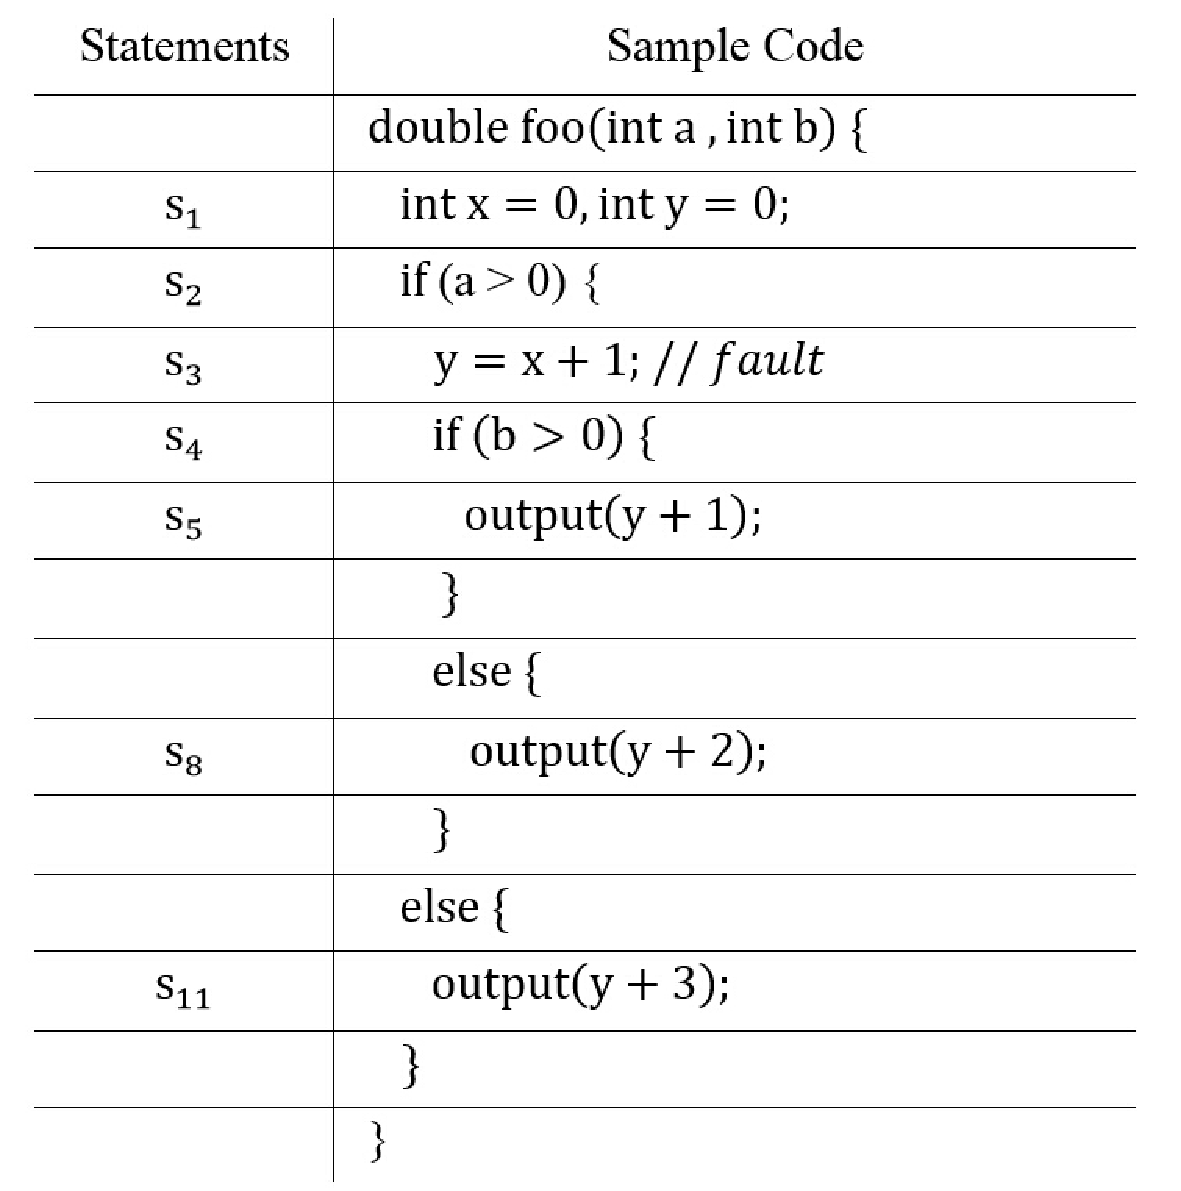
\includegraphics[width=0.6\textwidth]{chapter2_fig1.pdf}
\vspace {0em}\caption{Motivating Example} \label{fig2.1}
\end{center}
\vspace {0em}
\end{figure}

This problem, which is an instance of {\it confounding bias} (or just {\it confounding}) \cite{pearl2000models}, is due to the fact that execution of the control dependence region \cite{ball1993s} containing statements $s_3$ and $s_4$ is a {\it common cause} of program failure and of execution of statement $s_5$ or $s_8$.  More generally, confounding of the effect of a ``treatment" variable $T$ on an outcome variable $Y$ is bias due to the presence of a common cause $C$ of $T$ and $Y$.  Confounding bias cannot be eliminated, in general, without considering the causal relationships between the variables under study.  These relationships are typically represented in a {\it causal} DAG \cite{pearl2000models}, which is a directed acyclic graph in which there is an edge $A \rightarrow B$ just in case variable $A$ is a direct cause of variable $B$.  For example, Figure \ref{fig2.2} is a very simple causal graph showing the causal relationships between a treatment $T$, an outcome $Y$, and a confounder $C$.  For SFL, Baah et al \cite{baah2010causal,baah2011mitigating} proposed using a causal DAG derived from the {\it program dependence graph} (PDG) \cite{ferrante1987program}, in which the nodes represent binary coverage indicator variables.

Confounding can be reduced or eliminated by adjusting or controlling for a suitable set of variables during statistical analysis.  A well-known result of Pearl, the {\it Back-Door Adjustment Theorem} \cite{pearl2000models}, states that a set of covariates $\mathbf{X}$ in a causal DAG $G$ is sufficient for confounding adjustment if it ``blocks" all ``backdoor paths" between the treatment $T$ and the outcome $Y$.  A {\it backdoor path} between $T$ and $Y$ is a path with an arrow $T \leftarrow$ entering $T$.  A path is {\it blocked} by $mathbf{X}$ if the path (1) contains a configuration of the form $\rightarrow Z \rightarrow$ or $\leftarrow Z \rightarrow$ such that  $Z \in \mathbf{X}$or (2) contains a ``collider" $\rightarrow Z \leftarrow$  such that neither $Z$ nor any of its descendants is in $\mathbf{X}$.  For example, in Figure \ref{fig2.2} the path $T \leftarrow C \rightarrow Y$ is a backdoor path, which is blocked by $C$.

\begin{figure}[htb!]
\vspace{0em}
\begin{center}
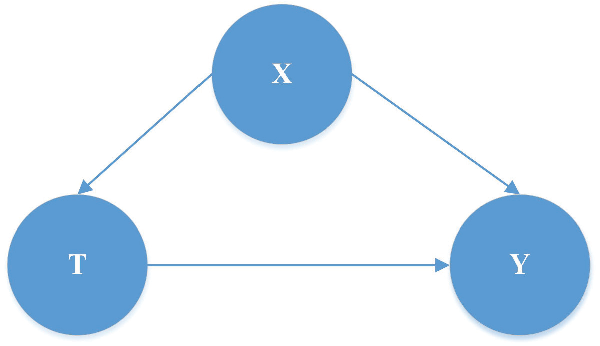
\includegraphics[width=0.6\textwidth]{chapter2_CausalDAG1.pdf}
\vspace {0em}\caption{Causal Diagram of treatment, outcome and confounder} \label{fig2.2}
\end{center}
\vspace {0em}
\end{figure}

\section{Contribution and organization of the dissertation}

This dissertation makes the following contributions: developed a novel value based approach to to SFL for numerical programs; analyzed two types of violations of positivity: structural violations and random violations in casual fault localization; the first use of BART model to estimate failure-causing effect for numerical expressions.

The remainder of the dissertation is organized as follows:

Chapter 2 investigates the performance of Baah et al’s causal regression model for fault localization when positivity condition is violated

Chapter 3 presents a value based causal inference model for localizing faults in numerical software called NUMFL, which use propensity score technique to control the confounding bias in fault localization.

Chapter 4 presents a new fault localization method based on Bayesian additive regression trees model.

Chapter 5 presents an approach to automatically localize faulty statements in the embedded control software.

Chapter 6 concludes this dissertation and discusses the possible improvements for future work.




\chapter{The Importance of the Positiity Property for CSFL}\label{chap:importance}

\section{Introduction}\label{sec1}
To adjust (partially) for confounding bias in {\it causal SFL} (CSFL), Baah et al proposed estimating the AFCE of a particular statement $s$ by using a linear regression model of the form
\begin{equation}\label{eq1}
Y=\beta_0+\beta_1T_s+\beta_2C_s+\sigma,
\end{equation}
where $\sigma$ is the treatment (coverage) indicator for $s$ (1: covered, 0: not covered); $C_s$ is a coverage indicator for the {\it forward control dependence predecessor} of $s$ \cite{ball1993s}, which we denote by $pred(s)$; $Y$ is a failure indicator (1: fails; 0: passes); $\beta_0$, $\beta_1$, and $\beta_2$ are coefficients, and $\sigma$ is a random error term.  (Model (1) is not applicable to $s$ if $pred(s)$ does not exist.)  Note that the units being ``treated" are program executions.  The covariate $C_s$ is used for confounding adjustment in this model because, in the forward control dependence subgraph of the PDG of a structured program, $pred(s)$ blocks all backdoor paths between $T_s$ and $Y$.  (It does not generally block backdoor paths involving data dependences, however.)  The AFCE estimate for $s$ is given by the estimated value $\widehat{\beta_1}$ of the coefficient $\beta_1$ of $T_s$ in model (1).  This estimate is used as the suspiciousness score of $s$.  Note that an instance of model (1) is fitted for each statement.  We shall refer to model (1) as Baah et al’s CSFL {\it regression model}.  (Note that Baah et al also proposed another approach to CSFL based on matching instead of regression \cite{baah2011mitigating}, and it does address data dependences.)

Interestingly, model (1) performed well when evaluated \cite{baah2010causal} even though the coverage data it requires often violates an important precondition for valid causal inference, called the ``positivity" condition.  In the remainder of this chapter, we shall examine why this is so and suggest improvements to Baah et al’s technique based on our conclusions.

\section{The Problem of Positivity Violations}\label{sec2}
Positivity \cite{hernan2006estimating} is an important condition for valid causal inference but is often overlooked in SFL research.

{\bf Definition.}  {\it The {\bf positivity} condition  holds with respect to a treatment variable $T$ and a set $X$ of covariates for confounding adjustment if the conditional probability $P(T=t|\mathbf{X=x})$ of receiving treatment value $t$, given the covariate values $\mathbf{X=x}$, is greater than zero for all $t$ and for all $\mathbf{x}$ such that $P(\mathbf{X=x})>0$.}
Suppose that $s$ is a statement with a unique forward control dependence predecessor $pred(s)$.  In terms of Baah et al's CSFL regression model \eqref{eq1}, positivity requires that, whether $pred(s)$ is covered ($C_s=1$) or is not covered ($C_s=0$), the probability of $s$ being covered ($T_s=1$) and the probability of $s$ not being covered ($T_s=0$) are both positive.  If either probability is zero then we say that the positivity condition is violated.

There are two distinct ways in which positivity can be violated [9, 10]:
\begin{itemize}
\item Structural violations of positivity occur if units with certain values of $\mathbf{X}$ cannot possibly be treated (or untreated).   For example, when the function in Figure \ref{fig2.1} is executed, if statements $s_3$ and $s_4$ are not covered then neither of statements $s_5$ and $s_8$ will be covered.  In the presence of structural nonpositivity, causal inferences cannot be made about the entire population of units.  The inference needs to be restricted to strata with $\mathbf{X}$ values for which structural positivity holds.

\item {\it Random violations} of positivity occur, in the absence of structural violations, due to sampling variability. That is, a sample is drawn containing some units with a value $\mathbf{x}$ of $\mathbf{X}$ such that for a certain treatment value $t$, no unit in the sample having $\mathbf{X=x}$ also has $T=t$.   For example, given a set of tests of the function in Figure \ref{fig2.1}, it may be that none of them covers statement $s_8$, even though it is possible to construct a test that does so.
\end{itemize}

\subsection{Research Questions}\label{question}
In the remainder of this chapter, we will consider three research questions concerning the existence of nonpositivity in CSFL and its consequence.

{\bf RQ1}: {\textit Is Baah et al’s causal inference model \eqref{eq1} subject to structural violations of positivity?  If so, how does this influence the AFCE estimates it yields?} In model \eqref{eq1}, $T_s$ and $C_s$ are both binary variables, so we might conceive of four different $(T_s,C_s)$ pairs: $(T_s=0,C_s=0)$, $(T_s=0,C_s=1)$,  $(T_s=1,C_s=0)$ and $(T_s=1,C_s=1)$.  However, $(T_s=1,C_s=0)$ cannot occur with execution data from a structured program, because if an execution does not cover $pred(s)$, it cannot cover $s$.  Thus $P(T_s=1|C_s=0)=0$, and so model \eqref{eq1} is subject to structural nonpositivity.  This means that it is impossible to identify the average causal effect of $T_s$ on $Y$ when $C_s$ is not restricted to be 1.  However, the empirical evaluation of model \eqref{eq1} reported by Baah et al \cite{baah2010causal}, as well as our own experimentation with the model, suggest that this does not seriously harm its fault localization performance in practice.  In Section III.A, we employ linear algebra to determine why this is so.

{\bf RQ2}: {\textit What are the consequences if model \eqref{eq1} is used despite random violations of positivity?}  Ideally, model \eqref{eq1} would be applied with execution data such that for each statement , both $(T_s=1,C_s=1)$ and $(T_s=0,C_s=1)$ occur.  This would be the case, for example, with a test set that achieves branch coverage.  In practice, however, it is possible that one or both of these pairs does not occur.  In this case, either the treated group of executions or the untreated group is empty.  If $s$ is not covered, there is no basis at all for estimating its AFCE.  This leaves the question of what to do if  is covered whenever $pred(s)$ is covered.  We examine this issue in Section III.B.

{\bf RQ3}: {\textit Given that model \eqref{eq1} is subject to structural nonpositivity, is the estimate $\hat{\beta_1}$ of the coefficient $\beta_1$ a valid causal effect estimate?}  In Section III.C, we present a probabilistic characterization of $\hat{\beta_1}$ that clarifies this issue. 

In Section IV, we also investigate RQ2 and RQ3 empirically.

\section{Analysis of the Research Questions}\label{sec3}
\subsection{Analysis of RQ1}\label{sec3.1}

In Section \ref{question}, we saw that Baah et al’s CSFL regression model \eqref{eq1} is subject to structural violations of positivity.  In this section, we analyze model \eqref{eq1} to see why this apparently does not harm its fault localization performance.  Let $\mathbf{y}$, $\mathbf{t}_s$, and $\mathbf{c}_s$ be column vectors of corresponding values of the failure indicator $Y$ and the coverage indicators $T_s$ and $C_s$, respectively, observed over a set of executions.  Let $\mathbf{1}$ be a column vector of $1$s of the same length $n$.  Let $\mathbf{X}$ be the matrix $[\mathbf{1}, \mathbf{t}_s, \mathbf{c}_s]$ and let $\mathbf{\beta}$ be the column vector $[\beta_0, \beta_1, \beta_2]'$ (we use $'$ here to indicate vector or matrix transpose). Then the regression model in equation \eqref{eq1} can be rewritten as
\begin{equation}\label{eq2}
\mathbf{y}=\mathbf{X} \bm{\beta}+\bm{\epsilon}
\end{equation}
where $\bm{\epsilon}$ is a column vector of random errors.

Assume that the parameters in model \eqref{eq2} are estimated by ordinary least squares.  Then the causal effect estimator $\hat{\beta_1}$ is given by \cite{johnson1992applied}
\begin{equation}\label{eq3}
\hat{\beta_1}=\frac{(cov(\mathbf{c}_s,\mathbf{c}_s )\cdot cov(\mathbf{t}_s,\mathbf{y})-cov(\mathbf{t}_s,\mathbf{c}_s )\cdot cov(\mathbf{c}_s,\mathbf{y}))}{(cov(\mathbf{t}_s,\mathbf{t}_s )\cdot cov(\mathbf{c}_s,\mathbf{c}_s )-cov(\mathbf{t}_s,\mathbf{c}_s )\cdot cov(\mathbf{t}_s,\mathbf{c}_s ) )}
\end{equation}
where $cov(\mathbf{a},\mathbf{b})$ denotes the covariance of sample vectors $\mathbf{a}$ and $\mathbf{b}$.  Letting the length of $\mathbf{a}$ and $\mathbf{b}$ be $n$, we have
\begin{equation}\label{eq4}
cov(\mathbf{a},\mathbf{b})=\frac{1}{n-1} \sum\nolimits_i (a_i-\mathbf{\overline{a}})(b_i-\mathbf{\overline{b}})
\end{equation}
Here, $\mathbf{\overline{a}}$ and $\mathbf{\overline{b}}$ denote the means of vectors $\mathbf{a}$ and $\mathbf{b}$, respectively.  Applying equation \eqref{eq4} to equation \eqref{eq3} and rearranging terms, the numerator of the quotient in equation \eqref{eq3} is:
\begin{equation}\label{eq5}
(\mathbf{c}_s \cdot \mathbf{c}_s)(\mathbf{t}_s \cdot \mathbf{y})-
(\mathbf{c}_s \cdot \mathbf{t}_s)(\mathbf{c}_s \cdot \mathbf{y})-
n {\overline {{\mathbf{c}_s}} ^2}(\mathbf{t}_s \cdot y)+
n{\overline {{\mathbf{c}_s}}}{\overline {{\mathbf{t}_s}}}(\mathbf{c}_s \cdot \mathbf{y})
\end{equation}
and the denominator of the quotient in equation \eqref{eq3} is
\begin{equation}\label{eq6}
(\mathbf{c}_s \cdot \mathbf{c}_s)(\mathbf{t}_s \cdot \mathbf{t}_s)-
(\mathbf{c}_s \cdot \mathbf{t}_s)^2-n {\overline {{t}_s} ^2}(\mathbf{c}_s \cdot \mathbf{c}_s)
-n{\overline {{c}_s} ^2}(\mathbf{t}_s \cdot \mathbf{t}_s)+2n \overline{\mathbf{c}_s}\overline{\mathbf{t}_s}
(\mathbf{c}_s \cdot \mathbf{t}_s)
\end{equation}
where $\mathbf{c}_s\cdot \mathbf{c}_s=\sum\nolimits_i {({c_{s,i}})} ^2$, 
$\mathbf{c}_s\cdot \mathbf{t}_s=\sum\nolimits_i {({c_{s,i}}{t_{s,i}})} $,
$\mathbf{c}_s\cdot \mathbf{y}=\sum\nolimits_i {({c_{s,i}}{y_i})}$, 
$\mathbf{t}_s\cdot \mathbf{t}_s=\sum\nolimits_i {({t_{s,i}})} ^2$, and
$\mathbf{t}_s\cdot \mathbf{y}=\sum\nolimits_i {({t_{s,i}}{y_i})}$ are scalar products and 
where $c_{s,i}$, $t_{s,i}$ and $y_i$ denote the values of $C_s$, $T_s$, and $Y$ for the $i$th 
execution, respectively.

From \ref{question}, we know that there are three possible $(T_s,C_s)$ pairs:
$(T_s=0,C_s=0)$, $(T_s=0,C_s=1)$, and $(T_s=1,C_s=1)$.  
However, when an execution has $(T_s=0,C_s=0)$, its corresponding $(c_{s,i})^2$, 
$c_{s,i}t_{s,i}$, $c_{s,i}y_i$, $(t_{s,i})^2$, and $t_{s,i}y_i$ values are all equal to 0, 
so that it makes no contribution to the values of the scalar products $\mathbf{c}_s\cdot\mathbf{c}_s$,
$\mathbf{c}_s\cdot\mathbf{t}_s$, $\mathbf{c}_s\cdot\mathbf{y}$, $\mathbf{t}_s\cdot\mathbf{t}_s$, 
and $\mathbf{t}_s\cdot\mathbf{y}$.  Such an execution makes no contribution to either the numerator \eqref{eq5} or the denominator \eqref{eq6} of the quotient in equation \eqref{eq3}.  
This implies that the value of the estimator $\hat{\beta_1}$ is determined solely by executions with
$(T_s=0,C_s=1)$ and $(T_s=1,C_s=1)$.  Provided that each of these pairs occurs for at least one execution, 
positivity holds for the stratum (group) of executions with $C_s=1$, since 
$P(T_s=0|C_s=1)>0$ and $P(T_s=1|C_s=1)>0$.  In this case $\hat{\beta_1}$ estimates the effect of the 
treatment variable $T_s$ on the outcome variable $Y$, given that $C_s$ is restricted to be 1.  
That is, $\hat{\beta_1}$ estimates the effect of covering $s$ on the occurrence of failures 
when $pred(s)$ is covered. Please check the Appendix for the detail of the derivation.


\subsection{Analysis of RQ2}\label{sec3.2}

In this section, we will discuss how random violations of positivity influence the performance of 
Baah et al’s CSFL model \eqref{eq1} and how to handle them.  As discussed in Section \ref{sec2}, 
random nonpositivity occurs when a statement $s$ is always executed $(T_s=1)$ or is never 
executed $(T_s=0)$ given that its forward control predecessor $pred(s)$ is covered $(C_s=1)$.  
In this case, the estimator $\hat{\beta_1}$ is not an unbiased estimator of the average 
failure-causing effect of  and may perform poorly as an SFL metric.  
The problem of random nonpositivity can be resolved by running additional test cases to increase code coverage.   
In case that is not practical, however, we consider what should be done instead.

Assume that for statement $s$, the treatment indicator $T_s$ is always equal to 1 given that $C_s=1$.  
Since $pred(s)$ is, by assumption, the unique forward control dependence predecessor of $s$, 
it must dominate $s$ in the program’s control flow graph (lie on all paths to $s$).  
Hence, if $pred(s)$ is not covered then $s$ cannot be covered either.  Consequently,  $T_s=C_s$ for all test cases. 
This will cause a collinearity problem \cite{wold1984collinearity} with the linear model \eqref{eq1}.  
A standard way to address this problem is to remove the variable $C_s$ from model \eqref{eq1} 
to obtain the following model:
\begin{equation}\label{eq7}
Y=\beta_0+\beta_1^* T_s+\epsilon
\end{equation}
The estimate $\widehat{\beta_1^*}$ plays the role of causal effect estimator.  
It is known that $\widehat {\beta _1^*} \approx P(Y = 1|{T_s} = 1)$ \cite{baah2010causal}.  
Since $T_s=C_s$, we also have that $\widehat {\beta _1^*} \approx P(Y = 1|{C_s} = 1)$.  
Thus, under random non-positivity, $\widehat{\beta_1^*}$ estimates the probability of failure given $C_s=1$.

\begin{figure}[htb!]
\vspace{0em}
\begin{center}
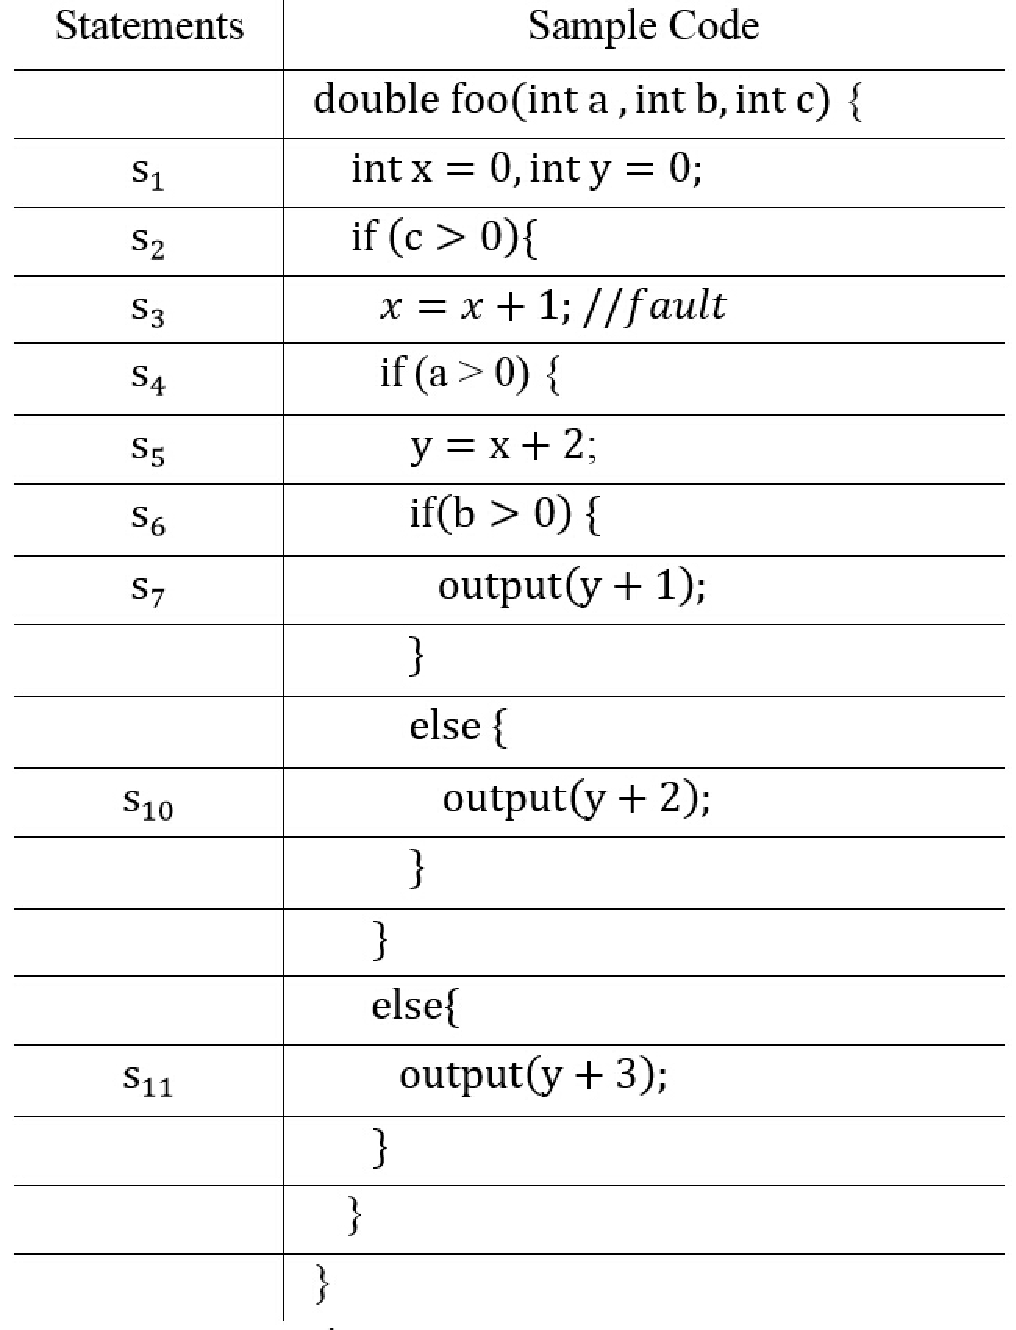
\includegraphics[width=0.6\textwidth]{chapter2_fig2.pdf}
\vspace {0em}\caption{Erroneous Program} \label{fig2.3}
\end{center}
\vspace {0em}
\end{figure}

Since model \eqref{eq7} does not adjust for confounding bias, $\widehat {\beta _1^*}$ may 
deviate from the failure causing effect of covering statement $s$.  For example, consider the program in Figure \ref{fig2.3}, which contains a faulty statement $s_3$, which should be $x=x+1$.  
Suppose that we want to estimate the failure causing effect of covering statement $s=s_7$.  
Assume that none of the observed executions cover statement $s_10$.  
This is a random violation of positivity, because $(T_{s_7}=0,C_{s_7}=1)$ is not observed.  
The estimator $\widehat{\beta_1^*}$ will be equal to $P(Y=1|C_{s_7}=1)$, where $pred({s_7})=s_6$.  
Because the faulty statement $s_3$ always executes before statement $s_6$ is executed, 
we have $P(Y=1|C_{{s_7}}=1)=1$, even though both $s_7$ and $s_6$ are correct.

To address random nonpositivity involving a target statement $s$ and $pred(s)$, 
we propose assigning the suspiciousness score of $pred(s)$ to statement $s$, 
provided that the causal effect estimator for $pred(s)$ adjusts for confounding.  
When random nonpositivity occurs, $s$ and $pred(s)$ have the same coverage information 
and thus their coverage-based suspiciousness scores should be same.  Referring again to Figure \ref{fig2.3}, 
the suspiciousness score of $s_7$ would be made equal to the suspiciousness score of $s_6$, 
which is estimated by model \eqref{eq1} with $T_s=s_6$ and $C_s=s_4$.  
We empirically evaluate this idea in Section \ref{sec4.2}.

\subsection{Analysis of RQ3}\label{sec3.3}
In this section, we will derive a probabilistic interpretation for causal effect estimator $\widehat{\beta_1}$.  
We first define some notation for different numbers of executions: $N_{T_s}=1$ is the number 
of executions with $T_s=1$; $N_{C_s}=1$ is the number with $C_s=1$; $N_{{C_s}=1,{T_s}=1}$ 
is the number with $C_s=1$ and $T_s=1$; $N_{{C_s}=1,Y=1}$ is the number with $C_s=1$ and $Y=1$; 
and $N_{{T_s}=1,Y=1}$ is the number with $T_s=1$ and $Y=1$.  Because $pred(s)$ dominates $s$ 
in the program’s control flow graph, we have
\begin{equation}\label{eq8}
N_{{C_s}=1,{T_s}=1}=N_{T_s=1}
\end{equation}
In addition, since $C_s$, $T_s$ are binary variables we have:
\begin{equation}\label{eq9}
{\mathbf{c_s}} \cdot {\mathbf{c_s}} = {\sum\nolimits_i {({c_{s,i}})} ^2} = {N_{C_s = 1}}
\end{equation}
\begin{equation}\label{eq10}
{\mathbf{c_s}} \cdot {\mathbf{t_s}} = {\mathbf{t_s}} \cdot {\mathbf{t_s}}
={\sum\nolimits_i {({t_{s,i}})} ^2} = {N_{T_s = 1}}
\end{equation}
\begin{equation}\label{eq11}
{\mathbf{c_s}} \cdot {\mathbf{y}} = {\sum\nolimits_i {c_{s,i}}y_i} = {N_{C_s= 1,Y=1}}
\end{equation}
\begin{equation}\label{eq12}
{\mathbf{t_s}} \cdot {\mathbf{y}} = {\sum\nolimits_i {t_{s,i}y_i}} = {N_{T_s= 1,Y=1}}
\end{equation}

With equations \eqref{eq8}-\eqref{eq12} we can rewrite the numerator \eqref{eq5} 
of the quotient in equation \eqref{eq3}, as
\begin{equation}\label{eq13}
\begin{array}{l}
N_{C_s=1}N_{T_s=1,Y=1}-N_{T_s=1}N_{C_s=1,Y=1}
-n{{\overline {\mathbf{c}_s}} ^2} N_{T_s=1,Y=1}
+n{\overline{\mathbf{c}_s}}{\overline{\mathbf{t}_s}}N_{C_s=1,Y=1}\\
=N_{C_s=1}N_{T_s=1,Y=1}-N_{T_s=1}N_{C_s=1,Y=1}
-\frac{{{N_{C_s=1}}^2}{N_{T_s=1,Y=1}}}{n}
+\frac{{N_{C_s=1}}{N_{T_s=1}}{N_{C_s=1,Y=1}}}{n}\\
=N_{C_s=1}N_{T_s=1,Y=1}(1-\frac{N_{C_s=1}}{n})-N_{T_s=1}N_{C_s=1,Y=1}(1-\frac{N_{C_s=1}}{n})\\
=(N_{C_s=1}N_{T_s=1,Y=1}-N_{T_s=1}N_{C_s=1,Y=1})(1-\frac{N_{C_s=1}}{n})
\end{array}
\end{equation}

Applying equations \eqref{eq8}-\eqref{eq12} to the denominator \eqref{eq6} in equation \eqref{eq3}, 
we can rewrite it as
\begin{equation}\label{eq14}
\begin{array}{l}
N_{C_s=1}N_{T_s=1}-{N_{T_s=1}}^2
-n{{\overline {\mathbf{t}_s}} ^2} N_{C_s=1}
-n{{\overline{\mathbf{c}_s}}^2}N_{T_s=1}
+2n{\overline{\mathbf{c}_s}}{\overline{\mathbf{t}_s}}N_{T_s=1}\\
=N_{C_s=1}N_{T_s=1}-{N_{T_s=1}}^2
-\frac{{{N_{T_s=1}}^2}{N_{C_s=1}}}{n}
-\frac{{{N_{C_s=1}}^2}{N_{T_s=1}}}{n}
+\frac{2N_{C_s=1}N_{T_s=1}}{n}\\
=N_{C_s=1}N_{T_s=1}-{N_{T_s=1}}^2+\frac{{{N_{T_s=1}}^2}{N_{C_s=1}}-{{N_{C_s=1}}^2}{N_{T_s=1}}}{n}\\
=N_{T_s=1}(N_{C_s=1}-N_{T_s=1})(1-\frac{N_{C_s=1}}{n})
\end{array}
\end{equation}

Given the derivations in \eqref{eq13} and \eqref{eq14}, equation \eqref{eq3} can be rewritten as follows:
\begin{equation}\label{eq15}
\begin{array}{l}
\widehat {\beta _1}=\frac{(N_{C_s=1}N_{T_s=1,Y=1}-N_{T_s=1}N_{C_s=1,Y=1})(1-\frac{N_{C_s=1}}{n})}{N_{T_s=1}(N_{C_s=1}-N_{T_s=1})(1-\frac{N_{C_s=1}}{n})}\\
=\frac{N_{C_s=1}N_{T_s=1,Y=1}-N_{T_s=1}N_{C_s=1,Y=1}}{N_{T_s=1}(N_{C_s=1}-N_{T_s=1})}\\
=\frac{N_{C_s=1}N_{T_s=1,Y=1}-N_{T_s=1}N_{T_s=1,Y=1}}{N_{T_s=1}(N_{C_s=1}-N_{T_s=1})}
-\frac{N_{T_s=1}N_{C_s=1,Y=1}-N_{T_s=1}N_{T_s=1,Y=1}}{N_{T_s=1}(N_{C_s=1}-N_{T_s=1})}\\
=\frac{N_{T_s=1,Y=1}}{N_{T_s=1}}-\frac{N_{C_s=1,Y=1}-N_{T_s=1,Y=1}}{N_{C_s=1}-N_{T_s=1}}
\end{array}
\end{equation}
Thus, the causal effect estimator $\widehat{\beta_1}$ is a difference of two terms:
\begin{equation}\label{eq16}
\frac{N_{T_s=1,Y=1}}{N_{T_s=1}}
\end{equation}
and
\begin{equation}\label{eq17}
\frac{N_{C_s=1,Y=1}-N_{T_s=1,Y=1}}{N_{C_s=1}-N_{T_s=1}}
\end{equation}
Let $N_{T_s=0,C_s=1}$ be the number of executions with $(T_s=0,C_s=1)$, and let $N_{T_s=0,C_s=1,Y=1}$ be the number of executions with $(T_s=0,C_s=1,Y=1)$.  Considering the relationship between $s$ and $pred(s)$, we see that
\begin{equation}\label{eq18}
N_{T_s=0,C_s=1}=N_{C_s=1}--N_{T_s=1}
\end{equation}
\begin{equation}\label{eq19}
N_{T_s=0,C_s=1,Y=1}=N_{C_s=1,Y=1}--N_{T_s=1,Y=1}
\end{equation}
Recall that $N_{C_s=1,T_s=1}=N_{T_s=1}$. Similarly, we have $N_{T_s=1,Y=1}=N_{C_s=1,T_s=1,Y=1}$.  Rewriting term \eqref{eq16}, we see that
\begin{equation}\label{eq20}
\begin{array}{l}
\frac{N_{T_s=1,Y=1}}{N_{T_s=1}}=\frac{\frac{N_{C_s=1,T_s=1,Y=1}}{n}}{\frac{N_{T_s=1}}{n}}\\
\approx \frac{P(T_s=1,C_s=1,Y=1)}{P(T_s=1,C_s=1)}\\
=P(Y=1|T_s=1,C_s=1)
\end{array}
\end{equation}
Applying equations \eqref{eq18} and \eqref{eq19} to term \eqref{eq17}, we see that
\begin{equation}\label{eq21}
\begin{array}{l}
\frac{N_{C_s=1,Y=1}-N_{T_s=1,Y=1}}{N_{C_s=1}-N_{T_s=1}}=\frac{\frac{N_{T_s=0,C_s=1,Y=1}}{n}}{\frac{N_{T_s=0,C_s=1}}{n}}\\
\approx \frac{P(T_s=0,C_s=1,Y=1)}{P(T_s=0,C_s=1)}\\
=P(Y=1|T_s=0,C_s=1)
\end{array}
\end{equation}
Hence,
\begin{equation}\label{eq22}
\widehat {\beta _1} \approx P(Y=1|T_s=1,C_s=1)-P(Y=1|T_s=0,C_s=1)
\end{equation}
This demonstrates that Baah et al’s AFCE estimator $\widehat{\beta_1}$ 
actually approximates the {\it associational risk difference} \cite{hernan2004definition} within 
the stratum of executions with $C_s=1$.  This measure is equal to the 
{\it causal risk difference} \cite{crump2006moving} within the stratum $C_s=1$ if the treatment 
effect of $T_s$ on $Y$ is unconfounded in that stratum.  Whether or not the 
last condition is true, $\widehat{\beta_1}$ is not an unbiased estimator of the 
AFCE over the whole population of executions.  This is consistent with our conclusions about structural nonpositivity in Section \ref{sec3.1}.  Note that if a random violation of positivity occurs, one of the two probability terms in equation \eqref{eq22} will be undefined, so $\widehat{\beta_1}$ will be undefined.

\section{Empirical Study}
We also conducted an empirical study of research questions RQ2 and RQ3.  We first describe the study platform and subject programs and then present the study results.


\subsection{Study Platform and Subject Programs}
{\bf Platform}: Our study platform is based on the JavaPDG dependence analysis tool \cite{shu2013javapdg} and the ASM Java bytecode manipulation framework \cite{ASM}.  To obtain the data required to use Baah et al’s model \eqref{eq1}, we first instrument a Java subject program’s class files using ASM, to record statement coverage information at runtime.  Then JavaPDG is used to generate a program dependence graph (PDG) of the subject program.  Each PDG node is mapped back to a source code statement.  For each statement , the PDG records the statement ID of $pred{s}$, if the latter exists.

{\bf Subject Programs}: We selected three subject programs written in Java: NanoXML, Rome, and Xerces2.  NanoXML \cite{Nanoxml} (version 1) is an XML parser from Software-artifact Infrastructure Repository (SIR) \cite{SIR}.  Rome (revision 840) is a open source library for parsing, generating, and publishing RSS and Atom feeds \cite{Rome}.  Apache Xerces2(v.2.9.1) is a processor for parsing, validating, serializing, and manipulating XML \cite{Xerces2}.  

{\bf Tests and Faults}: NanoXML comes with test suites.  To test Xerces2, XML files were collected from the system directories of an Ubuntu Linux 7.04 machine.  For Rome, test cases were obtained by downloading Atom and RSS files with a custom web crawler.  A sample of faults was selected randomly from the repository for each subject program: 4 for NanoXML, 5 for Rome, and 5 for Xerces2.  A summary of our subject programs and tests is shown in Table \ref{table1}.  

\begin{table}
\caption{Subject programs, tests, and faults}\label{table1}
\centering
\begin{tabular}{|c|c|c|c|}
\hline
Subject Program	&	LOC	&	Number of Tests	&	Faults	\\ \hline
NanoXML (SIR v1)	&	4.4K	&	1,000	&	4	\\ \hline
Rome (revision 840)	&	24K	&	2,000	&	5	\\ \hline
Xerces2 (v.2.9.1)	&	167K	&	1536	&	5	\\ \hline

\end{tabular}
\end{table}


\subsection{Evaluation of RQ2}\label{sec4.2}

To evaluate our conclusions about RQ2, we designed two sub-studies. The first sub-study was done to check whether random violations of positivity happen in practice. For a statement , such violations might occur in two ways: (1) no test executions have $(T_s=0,C_s=1)$, which means $s$ is always covered given $C_s=1$ and (2) no test executions have $(T_s=1,C_s=1)$, which means $s$ is never covered given $C_s=1$.  Note that in case (2), statement $s$ is never executed and so will not be assigned a suspiciousness score.  Thus, in our study we considered only case (2).  We also considered {\it only} statements $s$ for which $pred{s}$ exists.  Then we determined, for each subject program, which such statements were covered.  For each covered statement $s$, we checked if there were executions with $(T_s=0,C_s=1)$.  If not, a random violation of positivity, denoted RVP, occurred for $s$.  Table \ref{table2} shows the proportion of RVP statements among all covered statements for each subject program.  It shows that 4\% to 7\% of covered statements had random violations of positivity.

\begin{table}
\caption{Proportion of RVP statements among Covered statements with forward control dependence predecessor}\label{table2}
\centering
\begin{tabular}{|c|c|c|c|}
\hline
Subject Program	&	Number of RVP	&	Covered Statements	&	Proportion	\\ 
 & statements & with $pred(s)$ &\\\hline
NanoXML	&	19&	315	&	6.03\%	\\ \hline
Rome 	&	95	&	1353	&	7.02\%	\\ \hline
Xerces2 &	232	&	5545	&	4.18\%	\\ \hline

\end{tabular}
\end{table}

The second sub-study for RQ2 was done to determine if random violations of positivity affect the suspiciousness scores of statements.  The performance of Baah et al’s causal effect estimator $\widehat{\beta_1}$ was measured by the number of RVP statements assigned a ``bad" suspiciousness score.  We considered an RVP statement to have a bad suspiciousness score if its score was larger than  but the statement was not faulty or if its score was at most  but the statement was faulty.  In Section \ref{sec3.2}, we proposed assigning the suspiciousness score of $pred{s}$ to an RVP statement $s$.  Hence, we also checked if this ``adjusted" estimator performed better than $\widehat{\beta_1}$ under random violations of positivity.  Table \ref{table3} shows the number of RVP statement assigned “bad” suspiciousness scores by each estimator.  All the RVP statements of NanoXML had ``bad" suspiciousness scores.  For Xerces2, 207 out of 232 RVP statements had bad suspiciousness scores.  For Rome, RVP statements do not cause big problem: only 29 out of 95 RVP statements had bad suspiciousness scores.  When we applied the adjusted causal effect estimator, the numbers of RVP statements with bad suspiciousness scores dropped to 3 for NanoXML, to 23 for Rome, and to 102 for Xerces2.  The results suggest that the adjusted estimator performs better than the original one under random violations of positivity.
\begin{table}
\caption{Comparison between Baah et al’s  Original estimator and the ``Adjusted” estimator}\label{table3}
\centering
\begin{tabular}{|c|c|c|c|}
\hline
Subject Program	&	Number of RVP	&	Baah et al’s	&	Adjusted	\\ 
 & statements & estimator-bad scores &estimator-bad scores\\\hline
NanoXML	&	19&	19	&	3	\\ \hline
Rome 	&	95	&	29	&	23	\\ \hline
Xerces2 &	232	&	207	&	102	\\ \hline

\end{tabular}
\end{table}

\subsection{Evaluation of RQ3}
In Section \ref{sec3.3}, we have derived equation \eqref{eq22}, which is a probabilistic characterization of Baah et al’s estimator $\widehat{\beta_1}$.  An alternative estimator can be computed based directly on the right side of this equation, by replacing each probability by the corresponding sample proportion.  The two estimators should produce nearly identical suspiciousness scores.  To evaluate the correctness of equation \eqref{eq22}, we applied both estimators to the data from each of the subject programs.  We then computed the mean difference between these resulting scores, over all the statements of each subject program.  The result is shown in Table \ref{table4}.  We see that the mean difference is extremely small for each program, as is the variance of the difference.  Table \ref{table4} also shows the P-values of Student’s  tests of the null hypothesis of no difference in the score distributions, which are all 1 for each program. This indicates the means of each two groups of suspiciousness scores are statistically indistinguishable.

\begin{table}
\caption{Comparison between Baah et al’s  Original estimator and the ``Adjusted” estimator}\label{table4}
\centering
\begin{tabular}{|c|c|c|c|}
\hline
Subject Program	&	Mean	&	Variance	&	P-value	\\ \hline
NanoXML 	&	1.68E-16	&	1.25E-29	&	1	\\ \hline
Rome 	&	5.68E-16	&	8.05E-29	&	1	\\ \hline
Xerces2 	&	1.79E-16	&	7.64E-29	&	1	\\ \hline

\end{tabular}
\end{table}

We also measured the computation time for both estimators. The results are shown in Table \ref{table5}.  The probability-based causal effect estimator required substantially less computation time than the regression-based estimator, especially for the large subject program Xerces2.  

\begin{table}
\caption{Average execution times of regression-based causal effect estimator and probability-based causal effect estimator}\label{table5}
\centering
\begin{tabular}{|c|c|c|c|}
\hline
Subject Program	&	Regression	&	Probability	\\ \hline
NanoXML 	&	8.049 sec	&	4.354 sec	\\ \hline
Rome 	&	135.809 sec	&	44.308 sec	\\ \hline
Xerces2 	&	143.235 sec	&	54.578 sec	\\ \hline

\end{tabular}
\end{table}

\section{Related Work}
The most closely related work is on causal statistical fault localization techniques.  Baah et al \cite{baah2011mitigating} extended their original CSFL model by also controlling for confounding bias caused by data flow dependences, and they found this reduced localization costs.  Gore et al \cite{gore2012reducing} proposed an improved version of Baah et al’s original approach by providing a model that also addresses what they call {\it failure flow confounding bias}.  Shu et al \cite{shu2013mfl} proposed a CSFL technique for localizing faulty {\it methods} in large programs, which exploits dynamic call graph and dependence information and addresses nonpositivity.

Other related work examines positivity violations in causal inference generally.  Westreich, et al \cite{westreich2010invited} pointed out that positivity is important for making valid inferences from observational data but is often overlooked in practice, and they discussed general ways of dealing with nonpositivity.  Wang, et al \cite{wang2006diagnosing} analyzed the bias of an inverse-probability-of-treatment-weighted estimator in the face of positivity violations.  Petersen, et al \cite{petersen2010diagnosing} systematically reviewed how violations of positivity influence different types of causal-effect estimators.

Some recent studies have investigated methods for estimating causal effects in the presence of positivity violations. A ``trimming” technique is used in \cite{crump2006moving} is to discard units whose probability of treatment, conditional on covariates, is outside of a specified interval.  Another method proposed by Bembom et al  \cite{bembom2008data} is to exclude the confounders involved in positivity violations from the adjustment sets.  

\section{Conclusion}
Causal statistical fault localization techniques such as Baah et al’s CSFL regression technique can be biased when the positivity condition is violated \cite{bai2015importance}.  In this paper, we have analyzed two types of violations of positivity: structural violations and random violations. We established that structural violations do occur with Baah et al’s technique but are not harmful.  We proved that random violations also occur and that they can distort suspiciousness scores.  To address the problem of random nonpositivity, we proposed a modification to the way suspiciousness scores are assigned with Baah et al.’s technique.  Empirical results were presented that indicate it improves the technique’s performance. We also presented a probabilistic characterization of Baah et al’s estimator and showed that it provides a more efficient way to compute the same scores. Since Baah et al’s CSFL regression technique is based on a causal graph which omits data dependences, and since it characterizes program states only in terms of statement coverage, it does not eliminate all confounding bias in fault localization.  Nevertheless, it seems to perform well, and with our suggested improvements it is computationally efficient.











\chapter{Causal Inference Based Fault Localization for Numerical Software with NUMFL}\label{chap:NUMFL}

NUMFL is a value-based causal inference model for localizing faults in numerical software.  NUMFL combines causal and statistical analyses to characterize the causal effects of individual numerical expressions on output errors.  Given value-profiles for an expression's variables, NUMFL uses generalized propensity scores (GPSs) or covariate balancing propensity scores (CBPSs) to reduce confounding bias caused by evaluation of other, faulty expressions.  It estimates the average failure-causing effect of an expression using quadratic regression models fit within GPS or CBPS subclasses.  We report on an empirical evaluation of NUMFL involving components from four Java numerical libraries, in which it was compared to five alternative statistical fault localization metrics.  The results indicate that NUMFL is the most effective technique overall. We also found that NUMFL works fairly well with data from failing runs alone.

\section{Introduction}\label{introduction}
\vspace{-2pt}
Numerical software plays a very important role in science, industry, and defense, and failures of numerical software have been reported as the cause of several well-publicized ``disasters" \cite{VuikWeb,Kanewala2014}.  However, automated techniques intended specifically for localizing numerical faults based on execution data have received relatively little attention from researchers, although there has been substantial research on general {\it statistical fault localization} (SFL) techniques (e.g. \cite{Jones2002,Liblit2004,Liu2005}) and on other general automated debugging techniques (see Section \ref{relatedwork}).

Typical SFL techniques take data characterizing a set of both passing and failing program executions, including PASS/FAIL labels (provided by testers or end users) and recorded profiles of internal program dynamics, and they compute statistical measures of the strength of the association, if any, between the occurrence of software failures and the occurrence of certain runtime events at particular program locations.  These measures are then used to help guide the search for the causes of observed failures, typically by ranking program statements by the strengths of their associations with failures.  When SFL techniques are evaluated they are generally used as the sole source of information about possible fault locations.  However, it seems more realistic to envision them ultimately being used in combination with other sources of information, such as programmer hunches and {\it fault prediction models} \cite{Fenton1999} based on static code properties and project history.  Potentially, SFL techniques provide a relatively inexpensive way to maximize the information obtained by testing.

 In the vast majority of research on SFL, execution dynamics have been characterized either purely by {\it code-coverage profiles} (also called ``spectra"), indicating which statements, branches, or paths were covered by each execution (e.g., \cite{Jones2002}), or by indicators of the outcomes of {\it predicates} (e.g., \cite{Liblit2004}) – both existing branch predicates and predicates inserted specifically to enhance SFL (e.g., ones that compare the values of numeric variables to zero).  Although the outcomes of such predicates reflect the {\it values} of program variables, they may do so inadequately for SFL, e.g., because predicates or conditions are omitted mistakenly, because they are hidden in library code or microcode, or because few predicates are actually required in the program.  These facts make typical SFL techniques {\it poorly suited} for localizing faults in numerical programs and subprograms having relatively few conditional branches.  Even predicates inserted in a program to enhance SFL are likely to characterize the values of numeric variables inadequately, unless application-specific information is available that indicates which predicates should be inserted.

Although purely numerical programs, and numerical components of other programs, are often relatively small, the intricacy of their computations can make them very difficult to debug manually.  In order to provide automated fault localization assistance to developers who need to debug numerical programs or components, we present a new approach to SFL, denoted by {\it NUMFL}, that is designed specifically to localize faults in numerical code.  NUMFL, like some other recent work on SFL \cite{Baah2010,Baah2011, Gore2012,Shu2013}, is based on {\it causal inference methodology} \cite{Pearl2003}, which seeks to mitigate biases like confounding bias that can badly distort SFL scores used to guide the search for faults.  However, in contrast to previous work, NUMFL is based on generalized forms of {\it propensity scores} \cite{Imai2004,Imai2014}, which are a fairly recent development in causal inference that provide a means of reducing confounding bias when estimating the causal effect of a numeric {\it treatment} or {\it exposure} variable on an outcome variable.

In this chapter, each value of the ``treatment" variable $T_e$ is the result of evaluating a numerical expression or subexpression with a {\it unique program location} identified by $e$,   and the outcome variable $Y$ represents the error (possibly zero) in the output of the numerical program or component under consideration.  The causal effect of $T_e$ on $Y$ is characterized by a function $r_e (t)$, which in medical research is called a {\it dose-response function} (DRF) \cite{Hirano2004}.  To enable localization of faults, NUMFL summarizes the behavior of $r_e (t)$ over a set of evaluations of expression $e$, with a single quantity $susp(e)$ called a {\it suspiciousness score}. It employs generalized propensity scores to make it less likely that a correct expression will receive a high suspiciousness score because it used variables whose values were erroneous due to faults in {\it other} expressions. Note that we do {\it not} use propensity scores themselves as suspiciousness scores; the two kinds of scores have very different purposes.

We assume that (in most cases) users of NUMFL have a set of program or component inputs that induces multiple failing and multiple passing runs.  For these inputs, NUMFL requires corresponding {\it expected outputs} (not just PASS/FAIL labels) and execution profiles characterizing variable values.  The expected outputs are provided by testers or end-users, and the profiles are recorded automatically by program instrumentation.  To compute the suspiciousness score $susp(e)$,  NUMFL requires, in addition to values of the treatment variable $T_e$ and the output-error variable $Y$, corresponding values of the set of variables {\it used} in expression $e$.  Although the value-profiles used by NUMFL are more detailed than basic coverage profiles used by typical SFL techniques, the potential cost of recording and analyzing value profiles is offset by the relatively small size of many numerical programs.   Moreover, we assume that developer-time is a more critical resource in debugging than is computation time, because developers usually can do other work while an SFL algorithm runs.

The main contributions of this chapter are:
\vspace{-0.2cm}
\begin{itemize}
\item NUMFL, a new, value-based approach to SFL for numerical programs, which is based on sound causal inference methodology
	\item A new, value-based approach to SFL for numerical programs, named NUMFL, that is based on sound causal inference methodology, and two variants of NUML, denoted NUMFL-GPS and NUMFL-CBPS, based on alternative forms of generalized propensity scores
	\item The first use of generalized propensity scores to reduce confounding bias in SFL
	\item An implemented platform to profile the variables used and defined by numerical expressions in Java programs
\item An empirical comparison of NUMFL to five competing SFL techniques on components from four widely-used Java numerical libraries, which indicates that NUMFL is more effective overall than the other techniques
    \item Empirical evaluations of NUMFL on programs with single faults, with multiple faults, with both passing and failing executions, and with only failing executions
\item	An empirical comparison of NUMFL-GPS and NUMFL-CBPS to each other
\end{itemize}

This chapter is a revised and extended version of \cite{Bai2015}, which presented NUMFL-GPS, but not NUMFL-CBPS, and which evaluated NUMFL-GPS on only single-fault programs and with a mixture of passing and failing executions. The rest of the chapter is organized as follows: we present a motivating example in Section \ref{motivating}; background for our approach is presented in Section \ref{background}; NUMFL is described in detail in Section \ref{twoversion};  we report on its empirical evaluation in Section \ref{evaluation}; related work is surveyed in Section \ref{relatedwork}; and Section \ref{conclusion} concludes the chapter.

\section{Motivating Example}\label{motivating}

Figure \ref{code} shows a short function {\it harmean}, which correctly calculates the harmonic mean of two floating point numbers, in the middle column and shows a faulty version of {\it harmean} in the rightmost column.  (In real fault localization scenarios only the faulty code is usually available.)  We injected a fault into statement $s_3$ by adding a floating point number $c$ to the original expression $a*b$.  Given a pair of inputs $(a,b)$, the faulty version of $s_3$ produces an erroneous value for the variable $x$.  This value may propagate to statement $s_8$ and, via the variable $r$, cause an incorrect return value at statement $s_9$.  We use $r_{correct}$ and $r_{faulty}$ to denote the return value of the correct code and faulty code, respectively.  Let us assume that the faulty version of {\it harmean}, like many numerical programs, is considered to fail if the output error exceeds a predefined threshold $\epsilon$, that is, if

\begin{equation*}\label{threshold}
outerr = |{r_{correct}} - {r_{faulty}}| > \varepsilon
\end{equation*}

\begin{figure*}[!thpb]
\centering
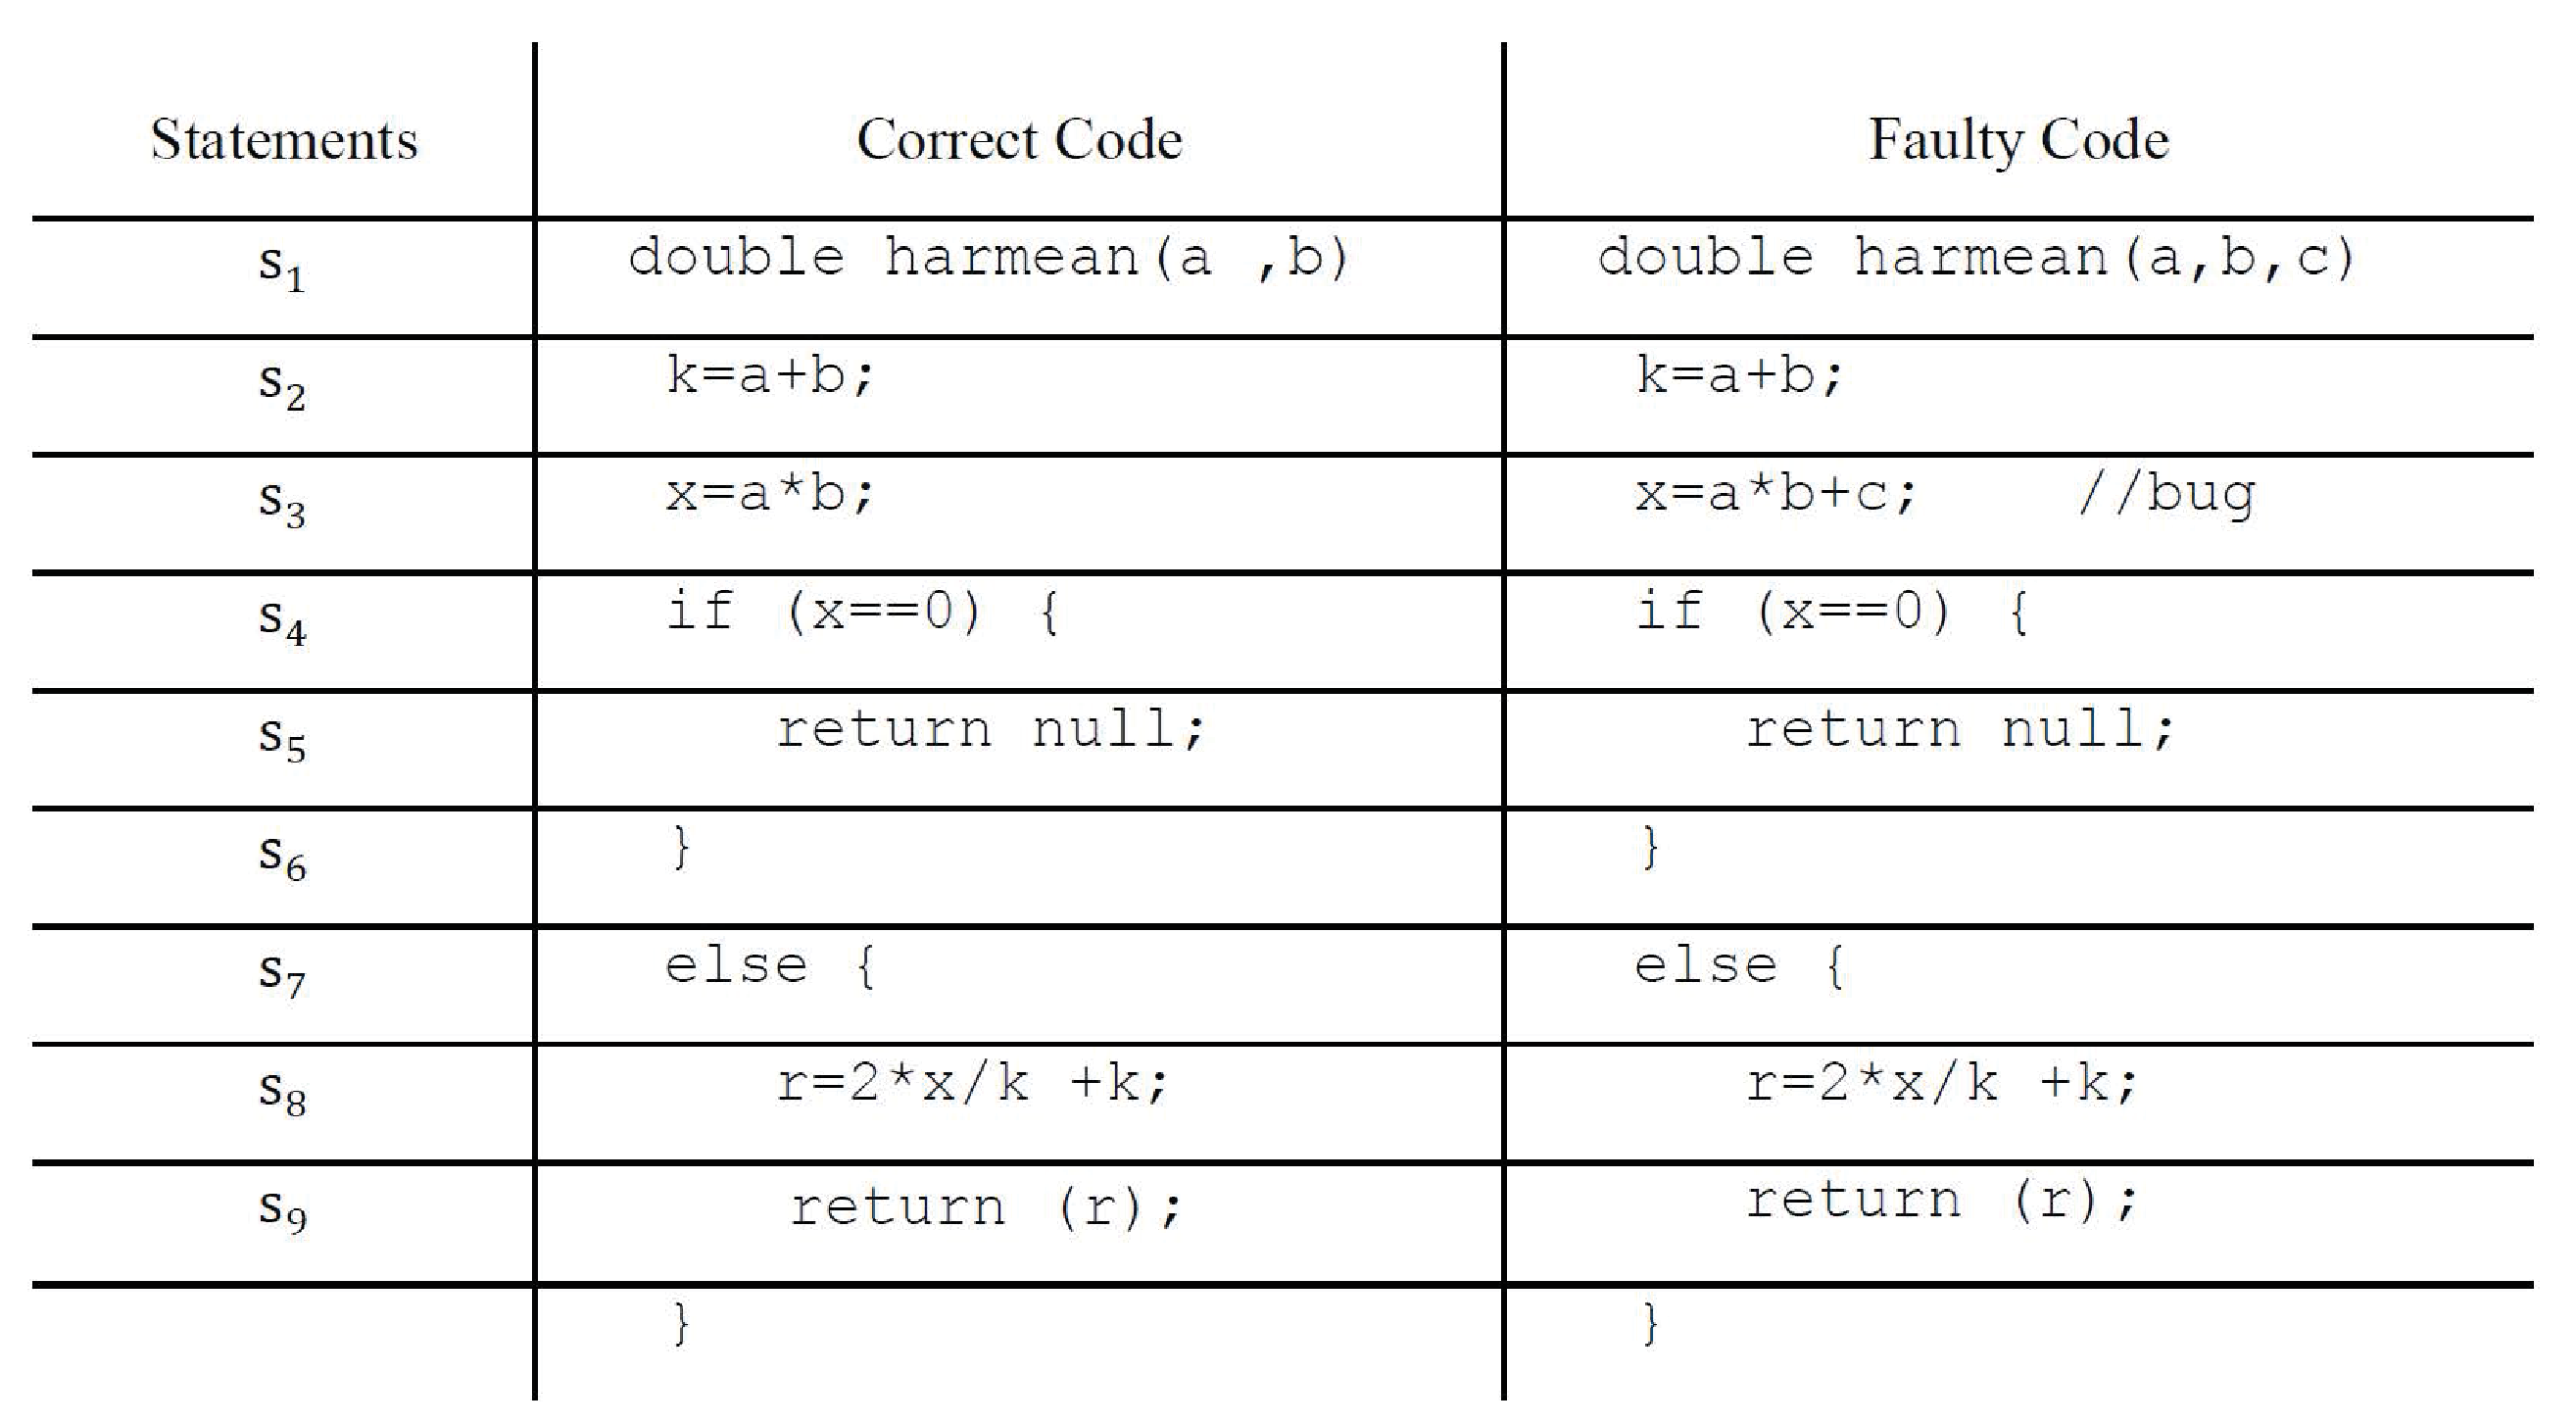
\includegraphics[width=0.8\textwidth]{MotivatingExample.eps}
\caption{Motivating Example}
\label{code}
\end{figure*}

Our goal is to automatically localize faults in numerical expressions, given variable-value profiles and expected outputs.  In the faulty code of Figure \ref{code}, there are three numerical expressions, in statements $s_2$, $s_3$ and $s_8$ , which define variables $k$, $ x$, and $r$.  A simple approach to detecting which expressions contain numerical faults is to obtain a ``suspiciousness" score for each numerical expression by calculating a measure of the statistical association between the values of the expression and the output error. This na\"{i}ve approach has two potential problems, however.  First, erroneous values due to a fault in one expression may propagate to other, correct expressions, causing them to receive high suspiciousness scores.  For example, in Figure \ref{code} the fault in statement $s_3$ causes variable $x$ to have erroneous values that propagate to statement $s_8$ and cause variable $r$ to have erroneous values. Consequently, the output error of {\it harmean} is associated with the values computed by both $s_3$ and $s_8$, even though $s_8$  is correct.  This problem, which is an instance of {\it confounding bias} (or {\it confounding}), is due to the fact that the computation of $x$ at $s_3$ is a {\it common cause} of program failure and of the computation of $r$ at $s_8$.  A na\"{i}ve measure of the association of $r$ with the output error, which does not account for confounding, will reflect both the true causal effect of $r$ on failure and the biasing effect of the confounder $x$ on $r$ and $outerr$.

The second problem with the na\"{i}ve approach is that common association measures like Pearson's correlation coefficient \cite{Philip2012} are often inadequate to measure the causal effect of a numerical expression on a program's output error, even without confounding.  For the example in Figure \ref{code},  $outerr=|r_{correct}-r_{faulty} |=|2c/(a+b)|$.  If $a=1$ and $b=0$, then $outerr=2|c|$ and $x=c$.  By definition, the correlation between $x$ and $outerr$ is:
\begin{equation*}\label{correlation}
%corr(x,outerr) = \frac{{{\mathop{\rm cov}} (x,outerr)}}{{{\sigma _x}{\sigma _{outerr}}}} = \frac{{{\mathop{\rm cov}} (c,2|c|)}}{{{\sigma _x}{\sigma _{outerr}}}}
corr(x,outerr) = \frac{{{\mathop{ cov}} (x,outerr)}}{{{\sigma _x}{\sigma _{outerr}}}} = \frac{{{\mathop{ cov}} (c,2|c|)}}{{{\sigma _x}{\sigma _{outerr}}}}
\end{equation*}
where $cov(x,outerr)$ is the covariance between $x$ and $outerr$ and where $\sigma_x$ and $\sigma_{outerr}$ are the standard deviations of $x$ and $outerr$, respectively.  Using basic covariance identities, we find that $cov(c,2|c|)=2cov(c,|c|)=2E[(c-\mu_c )(|c|-\mu_{|c|})]$, where $\mu_c$ and $\mu_{|c|}$ are the means of $c$ and $|c|$ respectively.  If the distribution of variable $c$ is symmetric about 0, $cov(c,|c|)$ is equal to 0, and so is $corr(x,outerr)$. Therefore, $corr(x,outerr)$ can be 0, even though the statement defining $x$ contains a fault.

NUMFL is intended to address the aforementioned problems and to provide less-biased estimates of the {\it failure-causing effect} of a numerical expression.  We now map the causal variables defined in the Introduction to the variables in our example:
\begin{enumerate}
\item 	Treatment variable $T_e$ is the variable defined in a numerical expression $e$.  In Figure \ref{code}, variables $k$, $x$ and $r$ are the treatment variables associated with statements $s_2$, $s_3$ and $s_8$, respectively.
	\item Outcome variable $Y$ is the absolute difference between the output of the faulty program and the expected (correct) output.  For the example, $Y$ is $outerr$.
\item $X$ represents the confounding variables, which are each causes of both treatment $T_e$ and outcome $Y$. For example, in the numerical expression $r=2*x/k$, the variables $x$ and $k$ are confounders because they each influence the values of both the treatment $T_e=r$ and the outcome $Y=outerr$.

\end{enumerate}

Figure \ref{dag1} shows the causal relationships between treatment, outcome, and confounding variables.
\begin{figure*}[!thpb]
\centering
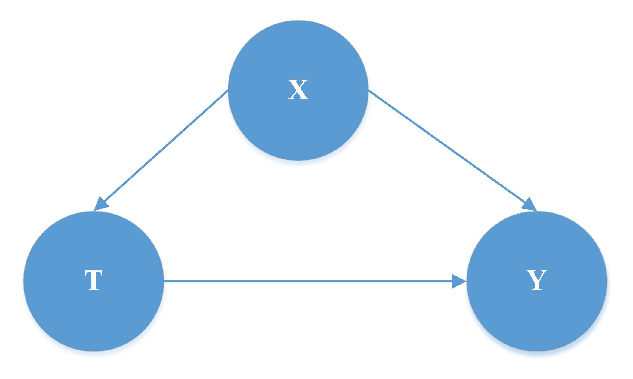
\includegraphics[width=0.5\textwidth]{CausalDAG1.eps}
\caption{Causal diagram of treatment, outcome, and confounder.}
%\vspace{-.5cm}
\label{dag1}
\end{figure*}


\section{BACKGROUND}\label{background}
\subsection{Causal Inference Methodology}\label{IIIA}
Causal inference methodology \cite{Pearl2003} has emerged in recent decades from research in a number of applied fields, to provide a basis for making valid inferences, from experimental or observational data, about the causal effects of specified treatments or exposures upon outcomes of interest.  Data about study variables is augmented with background knowledge about the causal relationships among variables, which is represented as {\it causal DAG}: a directed acyclic graph, in which nodes correspond to variables and in which there is an edge $A \to B$ if $A$ is an actual or assumed cause of $B$.  Causal inference theory establishes graph-theoretic conditions, such as Pearl's Backdoor Criterion \cite{Pearl2003}, under which a given causal effect can be estimated statistically without confounding or other forms of bias such as selection bias and measurement bias.



\subsection{Ordinary Propensity Scores}\label{IIIB}
Consider a treatment variable $T$ with two possible values 1 and 0.  (These values may indicate ``treated" and ``untreated", respectively, or they may indicate alternative treatments.)  One of the reasons that ideal randomized experiments, when they are feasible, are often considered the ``gold standard" for the design of causal inference studies \cite{Grossman2005} is that randomization makes it likely that the joint distribution of the covariates of the units with $T=1$ is similar to the covariate distribution of the units with $T=0$.  Such similarity, which is called {\it covariate balance} \cite{Rosenbaum1983}, implies that the two groups of units are comparable with respect to the values of confounding covariates, so that any difference in average outcomes of the groups is likely to be due to the treatment variable and not to confounding.  In randomized experiments, covariate balance is a consequence of the fact that the randomized treatment variable is {\it independent} of the covariates.

\begin{figure*}[!thpb]
\centering
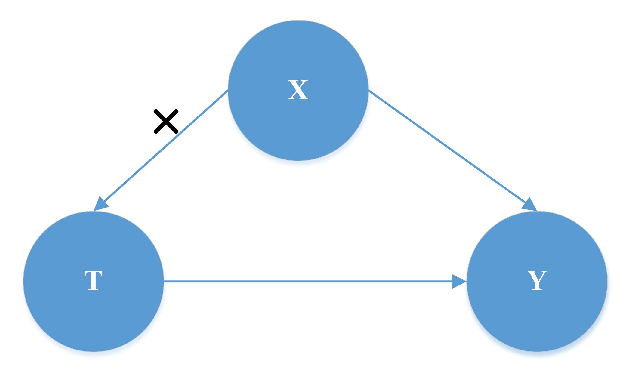
\includegraphics[width=0.5\textwidth]{CausalDAG2.eps}
\caption{Matching units based on their propensity scores breaks the link between cofounding variables and treatment.}
%\vspace{-.5cm}
\label{dag2}
\end{figure*}

An important approach to achieving covariate balance in observational studies is the use of (ordinary) {\it propensity scores} \cite{Rosenbaum1983}.  For a binary treatment variable $T$ and a vector of covariates $\pmb{X}$, the propensity score $Pr(T=1|\pmb{X}=\pmb{x})$ is the conditional probability of treatment $T=1$ given that the observed value of $\pmb{X}$ is $\pmb{x}$.  It has been shown that the propensity score is a {\it balancing score} in the sense that comparison groups with similar propensity scores tend to have similar covariate distributions \cite{Rosenbaum1983}.  True propensity scores are generally unknown, but they can be estimated from data about study units' actual treatment and covariate values.

Suppose that for each unit $i$ examined in an observational study, we have recorded the values of a binary treatment variable ${T_i} \in \{ 0,1\} $ and a vector of covariates ${\pmb{X}_i}$ .  We can use a parametric model ${\pi _{\pmb\beta} }({\pmb{X}_i})$ to estimate the propensity score for unit $i$.  One choice is the logistic model:

\begin{equation*}
{\pi _{\pmb\beta} }({X_i}) = Pr({T_i} = 1|{\pmb{X}_i}) = \frac{{\exp ({\pmb{X}_i}^\prime \pmb\beta )}}{{1 + \exp ({\pmb{X}_i}^\prime \pmb\beta )}}
\end{equation*}

We can estimate the parameter $\pmb\beta$ using maximum likelihood estimation \cite{Silvapulle1981}, which involves maximizing the log-likelihood function:

\begin{equation}\label{eq1}
{\pmb{\hat \beta} _{MLE}} = \arg \;\max \sum\limits_{i = 1}^N {{T_i}\log \left\{ {{\pi _{\pmb\beta} }({\pmb{X}_i})} \right\} + (1 - {T_i})} \log \left\{ {1 - {\pi _{\pmb\beta} }({\pmb{X}_i})} \right\}
\end{equation}

With the fitted model, we can estimate the ordinary propensity score  ${\pi _{\pmb\beta}}({\pmb{X}_i})$ for each observed unit.

After the propensity score model is estimated, covariate balance may be achieved by matching units based on their estimated propensity scores \cite{Rosenbaum1983}.  For example, each unit with $T=1$ can be matched to a unit with $T=0$ that has a similar estimated propensity score, if such a unit exists.  As illustrated in Figure \ref{dag2}, matching units based on their propensity scores breaks the link between the confounding variables and the treatment variable.

Ordinary propensity scores are not applicable to continuous treatment variables, however.  To address confounding of SFL scores for numerical expressions, we consider two variants of ordinary propensity scores that can accommodate continuous (and integer) treatment variables.  The first variant is the Generalized Propensity Score (GPS) proposed by Imai and Van Dyk \cite{Imai2004}.  The second variant is the Covariate Balancing Propensity Score (CBPS) proposed by Imai and Ratkovic \cite{Imai2014}.  Since CBPS is quite new, it has not been established whether it is superior to GPS.  Hence, we shall present and evaluate two versions of NUMFL, denoted NUMFL-GPS and NUMFL-CBPS, which are based on GPS and CBPS, respectively.  First, though, we briefly describe GPS and CBPS in the next two subsections.

\subsection{Generalized Propensity Score (GPS)}\label{IIIC}
The {\it Generalized Propensity Score} proposed by Imai and van Dyk \cite{Imai2004} is intended for use with any kind of treatment variable, including continuous ones.  Let ${p_{\pmb{\psi}} }(T|\pmb{X})$  be a model, with parameters $\pmb{\psi}$, of the {\it conditional probability density function} (p.d.f.) of the treatment variable $T$ given the covariate vector $\pmb{X}$.  The GPS for a specific unit with treatment level $T=t$ and covariate values $\pmb{X=x}$ is the density value $r = {p_{\pmb\psi} }(T = t|{\pmb X} = {\pmb x})$.  Imai and van Dyk \cite{Imai2004} require that the model ${p_{\pmb{\psi}} }(T|\pmb{X})$ has a {\it unique parameter} ${\pmb\theta}  = \pmb{\theta _\psi }(X)$ such that ${p_{\pmb{\psi}} }(T|\pmb{X})$ {\it depends on} $\pmb X$ {\it only through} $\pmb \theta$.  For example, if the treatment is represented by a {\it linear Gaussian model} $T|\pmb{X} \sim {\cal N}(\pmb{X}'{\pmb \beta} ,{\sigma ^2})$ with mean $\pmb{X}'{\pmb \beta}$  (the scalar product $\pmb{X}$-transpose times $\pmb{\beta}$) and variance $\sigma ^2$, so that $\pmb{\psi}  = \left( {\pmb{\beta} ,{\sigma ^2}} \right)$, then $\pmb{\theta}  = \pmb{X}'\pmb{\beta} $ (here $\pmb{\theta} $ is scalar).  The model parameters $\pmb{\psi}$, $r$, $\pmb{\theta}$, $\pmb{\beta}$, etc. are estimated from data; the corresponding estimates are denoted with by $\hat {\pmb\psi} $, $\hat r$, $\hat{ \pmb{\theta}} $, $\hat{ \pmb{\beta}}$, etc..  In Imai and van Dyk's approach, it is the values of the parameter estimate ${{\hat{\pmb{\theta}} }_{\hat{ \pmb{\psi}} }}(\pmb{X})$ that are used to control confounding, rather than the values of ${p_{\hat{ \pmb{\psi}} }}(T|\pmb{X})$ themselves.

Table \ref{exampledata} lists 10 test cases of faulty code in the motivating example. The three inputs $a$, $b$ and $c$ are generated randomly in the range $[-5, 5]$.  Table \ref{exampledata} also shows the values of intermediate variables values of $k$ and $x$ which are defined in expressions $s_2$ and $s_3$ respectively. The variable $r$ in expression $s_8$ is the faulty code's output and the variable $r_c$ represents the output of the correct code in motivating example with the same inputs. Outcome variable $Y$ is equal to $|r-r_c|$, so all the values of $Y$ are positive in the table. All the values in the table are rounding to three decimals. We use expression $s_8$ as an example to demonstrate generalized propensity score is estimated. For expression $s_8$, the treatment variable $T_e$ is variable $r$ and the confounding variables $\pmb{X}$ are covariates $x$ amd $k$. We first fit a linear regression model $T_e = \beta_0+{\beta_1}x+{\beta_2}k$ with $r $ as response, $x$ and $k$ as predictors. Given the data in Table \ref{exampledata}, the fitted regression model is $ T_e =0.614x+1.212k-1.462$. Then we estimate GPS ${{\hat{\pmb{\theta}} }_{\hat{ \pmb{\psi}} }}(x, k)$  by inputting observed value of $x$ and $k$ into the fitted regression model.  The estimated GPS for expression $s_8$ is denoted by$ {\hat{\theta}}_{s_8} $and is shown in the last column of the table.  

The confounding variables' effect on treatment variable can be controlled if conditioned on GPS. This can be proved with the data in Table\ref{exampledata}. For the confounding variable $x$'s effect on treatment variable $r$, we fit two regression models: the first model uses $r$ as respond and $x$ as predictor; the second model uses $r$ as respond, but uses both $x$ and GPS ${\hat{\theta}}_{s_8}$ as predictors. Given the data in Table\ref{exampledata}, the first model is fitted as $ r =0.487x-1.729$ and the second model is fitted as $r=-2.271E^{-16}x+ 1.0{\hat{\theta}}_{s_8}-1.461$. In the first model, the coefficient of $x$ means the variable $r$ will increase 0.487 if $x$ increased 1 unit. In the second model, the coefficient of $x$ is close to 0, while the coefficient of propensity score ${\hat{\theta}}_{s_8}$ is 1. This means the variable value of $r$ is mostly depend on the value of  ${\hat{\theta}}_{s_8}$. Similarly, we can have another two fitted model for the other confounding variable $k$: $r=0.999k-1.415$  and $r=-2.755E^{-16}k+1.0{\hat{\theta}}_{s_8}$-1.461.  The coefficient of $k$ is also reduced to 0 in the second model.  Thus, given GPS, the effect of confounding variables on treatment variable is significantly reduced, which can also be illustrated by Figure \ref{dag2}

\begin{table*}[htbp!]
\caption{VARIABLE VALUES AND GPS OF THE MOTIVATING EXAMPLE}
\label{exampledata}
\centering
      \begin{tabular}{|l|c|c|c|c|c|c|c|c|c|c|}
      \hline
Test \#	&1	&2&3&4 & 5 &6& 7 & 8 & 9&10\\	\hline

$a$ &-1.697	&	4.088	&	0.242	&	-0.269	&	-3.495	&	-2.081	&	-2.063	&	-2.896	&	3.839	&	-3.412 \\ 	\hline
$b$ & -1.430	&	0.660	&	4.843	&	-1.803	&	-3.352	&	1.282	&	-1.520	&	4.568	&	1.796	&	0.325\\	\hline
$c$ & -3.990	&	3.778	&	-2.242	&	-0.347	&	-1.678	&	-0.358	&	3.766	&	-4.690	&	-2.535	&	-1.645 \\	\hline
$k$ & -3.127	&	4.748	&	5.084	&	-2.072	&	-6.847	&	-0.799	&	-3.583	&	1.672	&	5.636	&	-3.088\\	\hline
$x$ &-1.564	&	6.478	&	-1.071	&	0.138	&	10.036	&	-3.025	&	6.902	&	-17.919	&	4.362	&	-2.752 \\	\hline
$r $& -2.127	&	7.477	&	4.663	&	-2.205	&	-9.778	&	6.777	&	-7.436	&	-19.768	&	7.184	&	-1.305\\	\hline
$r_c$ & -4.679	&	5.885	&	5.545	&	-2.540	&	-10.268	&	5.881	&	-5.334	&	-14.157	&	8.083	&	-2.371 \\	\hline
$Y$ & 2.552	&	1.592	&	0.882	&	0.335	&	0.490	&	0.896	&	2.102	&	5.611	&	0.900	&	1.065 \\	\hline
${\hat{\theta}}_{s_8}$ & -4.749	&	9.731	&	5.502	&	-2.426	&	-2.132	&	-2.825	&	-0.102	&	-8.978	&	9.506	&	-5.431\\	\hline

\end{tabular}
\end{table*}


\subsection{Covariate Balancing Propensity Score (CBPS)}\label{IIID}
Section \ref{IIIB} explained that the ordinary propensity score is a balancing score and that it can be estimated from data using a parametric statistical model.  However, if the propensity score model ${\pi _{\pmb \beta} }({\pmb{X}_i})$  is {\it misspecified}, matching on the estimated propensity scores (and related techniques) may fail to balance the covariates, yielding biased estimates of causal effects. To address this problem, Imai and Ratkovic proposed the {\it Covariate Balancing Propensity Score} (CBPS), which is robust to mild misspecification of the propensity score model \cite{Imai2014}.
The CBPS optimizes covariate balance by modifying the estimation procedure for parameter $\pmb{\beta}$ .  Differentiating equation \eqref{eq1}, equating the result to zero, and taking expectations, we have \cite{Imai2014}
\begin{equation}\label{eq2}
E\left\{ {\frac{{{T_i}{{\pi '}_{\pmb \beta} }({\pmb{X}_i})}}{{{\pi _{\pmb \beta} }({\pmb{X}_i})}} - \frac{{(1 - {T_i}){{\pi '}_{\pmb \beta} }({\pmb{X}_i})}}{{1 - {\pi _{\pmb \beta} }({\pmb{X}_i})}}} \right\} = 0,
\end{equation}
where ${\pi '_{\pmb \beta} }({\pmb{X}_i}) = \partial {\pi _{\pmb \beta} }({\pmb{X}_i})/\partial \pmb{\beta}$.  Equation \eqref{eq2} is called a {\it balancing condition} or a {\it moment condition} \cite{Imai2014}.  (The mean of a random variable is its ``first moment" \cite{Rosenblueth1981}.)  In CBPS, the balancing condition is generalized as
\begin{equation}\label{eq3}
E\left\{ {\frac{{{T_i}{{\tilde {\pmb X}}_i}}}{{{\pi _{\pmb \beta} }({\pmb{X}_i})}} - \frac{{(1 - {T_i}){{\tilde {\pmb X}}_i}}}{{1 - {\pi _{\pmb \beta} }({\pmb{X}_i})}}} \right\} = 0,
\end{equation}
where ${\tilde {\pmb X}_i} = f({\pmb{X}_i})$ represents a vector-valued function of the covariates $\pmb{X}_i$. To ensure that the first moment of each covariate is balanced, even when the model is misspecified, we can set ${\tilde {\pmb X}_i} = {\pmb{X}_i}$. CBPS employs a parameter estimation framework called the {\it generalized method of moments} (GMM) \cite{Hansen1982}, which is based on solving moment-condition equations for the parameters of interest and substituting sample moments for unknown population moments. Imai {\it et al}. extended CBPS to treatments with $K>2$ integer values, using a $multinomial\;model$ for the conditional probability of treatment given the covariates. We adapted this approach slightly to make it applicable to value-based fault localization (see Section \ref{IVB}), and we evaluate CBPS in NUMFL as an alternative to GPS .

\section{TWO VERSIONS OF NUMFL}\label{twoversion}
In this section, we define two versions of NUMFL, NUMFL-GPS and NUMFL-CBPS, and explain how they are used to reduce confounding bias during estimation of a numerical expression's {\it average failure-causing effect} (AFCE). Intuitively, an aggregate measure of the failure-causing effect of a numerical expression $e$ should summarize the effects on output errors of evaluating $e$ over a sample of program runs that each cover or reach $e$. Accordingly, in causal inference the designated ``treatment" variable $T_e$ should reflect the values produced by individual evaluations of $e$. (Of course $e$ may be evaluated repeatedly in a single program run, due to iteration.) Runs that do not reach $e$ are {\it not relevant} to such a measure. This is unlike measures of the failure-causing effect of covering a statement $s$ at least once during a run (e.g., \cite{Jones2002}), which contrast runs that cover $s$ with runs that don't cover $s$. With such measures, the treatment variable indicates whether or not $s$ was covered during a given run.

Recall that confounding of the causal effect of a treatment variable $T$ upon an outcome variable $Y$ is bias that is due to the presence of one or more common causes of $T$ and $Y$. The influence of such a common cause $X$ can make the effect of $T$ on $Y$, as reflected by a na\"{i}ve measure of statistical association, appear to be stronger or weaker than it really is. As mentioned in Section \ref{IIIB}, ordinary propensity scores cannot be used in causal inference to control confounding when the treatment variable is continuous.  Since the ``treatments" that NUMFL deals with are the values of numeric program variables, we instead define and evaluate two versions of NUMFL, namely NUMFL-GPS and NUMFL-CBPS, that are based respectively on GPS and CBPS, the two generalizations of ordinary propensity scores described in Sections \ref{IIIC} and \ref{IIID}.

\subsection{NUMFL-GPS}\label{IVA}
As with ordinary propensity scores, GPS is used to control for statistical associations between the treatment variable and confounding covariates, which in the case of NUMFL are variables used (read) in a numeric expression $e$ whose AFCE we wish to estimate. In general, these program variables are potential confounders because they may contain erroneous values just before expression $e$ is evaluated, due to faults in previously evaluated expressions. If these erroneous values cause program failures (that is, ``coincidental correctness" does not occur) the result of evaluating $e$ may be strongly associated with failures even if $e$ is correct, unless steps are taken to control confounding. In NUMFL, therefore, when estimating the AFCE of $T_e$ on the output error $Y$, we control for the values of the variables used in $e$.  (Those familiar with Pearl's Backdoor Adjustment Criterion \cite{Pearl2003} should note that this breaks any backdoor paths between $T_e$ and $Y$ in the acyclic data flow graph induced by a program execution.)

\subsubsection{Control of Confounding.}
For a given numerical expression $e$ in a program, NUMFL-GPS currently fits a linear
Gaussian GPS model ${{\pmb T}_e}|{{\pmb X}_e} \sim N({\pmb X}_e'{{\pmb \beta} _e}, \sigma _e^2)$ , where the treatment variable $T_e$ represents the result of evaluating $e$ (once) and where the possibly confounding covariates in the vector $\pmb{X}_e$ represent the corresponding values of the program variables used in evaluating $e$. Observe that one program run may generate multiple values of $T_e$ and $\pmb{X}_e$, due to iteration. To reduce profiling overhead, these may be sampled rather than recorded exhaustively. We currently sample only the values from the {\it last iteration} of a loop.

Applying GPS in NUMFL entails the following three steps:
\begin{enumerate}
\item 	Given a sample of observed values for the treatment variable $T_e$ and for the covariates $\pmb{X}_e$, fit a linear regression model $T_e=\pmb{X}_e' \pmb{\beta}_e$ to obtain the estimated parameter vector $\hat {\pmb{\beta}}_e$.
\item For each observed value ${\pmb x}_{e,i}$ of $\pmb{X}_e$, compute the estimate ${{\hat \theta }_{e,i}} = {\pmb{x}_{e,i}}'{{\hat {\pmb{\beta}} }_e}$.
\item Group observations with the same or similar values of $\hat{\theta}_{e,i}$ into $m$ subclasses of roughly equal size.
\end{enumerate}

The regression model fitted in the first step characterizes how the values of the covariates in $\pmb{X}_e$ influence the value of the treatment variable $T_e$.  In the second step, $\hat{\theta}_{e,i}$ estimates this influence for a particular value $\pmb{x}_{e,i}$ of $\pmb{X}_e$.  The scalar $\hat{\theta}_{e,i}$ summarizes the influence of the vector value $\pmb{x}_{e,i}$ on the treatment, and hence $\hat{\theta}_{e,i}$ may be used in place of $\pmb{x}_{e,i}$ for confounding control. Accordingly, in the third step, each subclass of observations with similar $\hat{\theta}_{e,i}$ values corresponds to a set of $\pmb{x}_{e,i}$ values that influence the treatment similarly. Thus, within each subclass, there is little or no association between confounders and the treatment variable $T_e$.

To illustrate this procedure, we refer again to the faulty version of the function {\it harmean} in Figure \ref{code}.  Statement $s_8$ is $r=2*x/k +k$. To control possible confounding of the average failure-causing effect of $r$ by the variables $x$ and $k$, we first fit a linear model $r=\beta_1 z+\beta_2 k$, where $z=x/k$, using a sample of corresponding observed values $(r_i,x_i,k_i)$. Second, we apply the fitted model to each pair $(x_i,k_i)$ to obtain a predicted value $\hat \theta_i$.  Third, we group the observations with similar $\hat \theta_i$ values into subclasses. This can be done by sorting the $\hat \theta_i$ into descending order and partitioning the sorted values into $m$ roughly equal-size bins.

Although GPS can control confounding bias caused by multiple confounding covariates, there is one challenge to applying it in NUMFL-GPS. If the dimension of $\pmb{X}_e$ is high, the first step of GPS requires a large number of observations to fit a suitable regression model.  In practice, a numerical expression defined by a statement could contain more than 10 confounders, but the number of tests may not be large enough to fit the regression parameters with adequate precision. Thus, to apply GPS, we need to control the dimension of confounding variables.

To address this problem, we $decompose$ a complex numerical expression into several subexpressions, each involving operators with the same precedence level.  For example, a numerical statement $a=(b+c+d)*e$ will be decomposed into two subexpressions: (1) $temp=b+c+d$ and (2) $a=temp*e$.  Here, $temp$ is a temporary variable that plays the role of the treatment variable for subexpression (1) and the role of a possible confounder for subexpression (2). Thus, each subexpression has fewer confounding variables and a relatively simple structure.  For each subexpression, we use GPS to control confounding bias and then estimate the subexpression's AFCE.

\subsubsection{Failure-causing Effect Estimation.}
Within each of the subclasses created by grouping observations with similar $\hat \theta_i$ values, the treatment values $T_{e,i}$ should be largely independent of the covariate values $\pmb{X}_{e,i}$, provided that the GPS model is adequate. Hence, the relationship between the treatment variable $T_e$ and the outcome variable $Y$ should be nearly unconfounded in each subclass. If this relationship is roughly linear in each subclass, we can estimate the expected dose-response function $E[Y|T_e]$ {\it within a particular subclass} using a simple linear regression model \cite{Zhao2013}:
\begin{equation}\label{lrm}
Y=\gamma_eT_e+b
\end{equation}
Recall that $Y$ is the absolute difference between the output of the faulty program and the expected (correct) output. In equation \eqref{lrm}, $b$ is a constant intercept. The coefficient $\gamma_e$ is the slope of $E[Y|T_e]$. It indicates how much the expected value of the outcome variable changes when the treatment value increases by one unit. The slope coefficient $\gamma_e$ can be estimated by the least-squares estimator $\hat \gamma_e$:
\begin{equation}\label{ls}
\hat \gamma_e=({\pmb t}_e'{\pmb t}_e)^{-1}{\pmb t}_e'{\pmb y},
\end{equation}
where $\pmb{t}_e'$ is the transpose of the vector of treatment values and where $\pmb y$ is the vector of outcome values (output errors).

Intuitively, an association measure used as an SFL suspiciousness metric for numerical programs should, when applied to a numerical expression $e$, reflect the likelihood that $e$ is faulty.  Although the coefficient estimate $\hat \gamma_e$ summarizes the dose-response function, it is not an adequate SFL metric, because of the {\it symmetry} of many numerical errors. For example, suppose that $Y=|T_e |$.  Since the output error $Y$ is completely determined by $T_e$, expression $e$ should receive a high suspiciousness score. However, if the value of $T_e$ is distributed symmetrically around zero, then $\hat \gamma_e$ will be close to zero, which suggests misleadingly that $e$ has no causal effect on program failures.

To derive a better suspiciousness metric, we first analyze the relationship between a numeric fault and the DRF slope estimator $\hat \gamma_e$. Assume that the numeric expression $e$ has a fault, which results in erroneous treatment values represented by the treatment variable $T_e^f=T_e$.  Let the treatment variable $T_e^c$ represent the corresponding treatment values in the correct program. Then we have $T_e^f=T_e^c+\varepsilon_e$, where $\varepsilon_e$ is a treatment error term.  Then $\hat \gamma_e $ may be decomposed as follows:

\begin{equation}\label{decomp}
\begin{array}{l}
{{\hat \gamma}_e} = {({{\pmb t}_e^f}'{\pmb t}_e^f)^{ - 1}}({\pmb t}_e^c + {{\pmb \varepsilon} _e})'{\pmb y}\\
 = {({{\pmb t}_e^f}'{\pmb t}_e^f)^{ - 1}}{{\pmb t}_e^c}'{\pmb y} + {({{\pmb t}_e^f}'{\pmb t}_e^f)^{ - 1}}{{\pmb \varepsilon} _e}^\prime {\pmb y}\\
 = {{\hat \gamma}_e}^c + {{\hat \gamma}_e}^f,
\end{array}
\end{equation}
where $\pmb{t}_e^f$, $\pmb{t}_e^c$, and ${\pmb \varepsilon}_e$ are the vectors of sample values for $T_e^f$, $T_e^c$, and $\varepsilon_e$, respectively, and where ${{\hat \gamma}_e}^c  = {({{\pmb t}_e^f}'{\pmb t}_e^f)^{ - 1}}{{\pmb t}_e^c}'{\pmb y} $ and ${{\hat \gamma}_e}^f = {({{\pmb t}_e^f}'{\pmb t}_e^f)^{ - 1}}{{\pmb \varepsilon} _e}^\prime {\pmb y}$. The component $\hat \gamma _e^f$ of ${\hat \gamma _e}$ characterizes the causal relationship between the treatment error $\varepsilon_e$ and the output error $Y$. If $\varepsilon_e$ is symmetrically distributed then the contributions to $\hat \gamma _e^f$ of the positive and negative values of $\varepsilon_e$ will tend to cancel each other, since $Y$ is an absolute value, leaving $\hat \gamma _e^f$ close to zero.

We have considered two possible approaches to this problem.  We call the first of these a {\it dual linear regression model} (DLRM).  The basic idea of DLRM is simple: compute
$|\hat \gamma _e^f|$ separately for positive $\varepsilon_e$ and for negative $\varepsilon_e$ and then add the two resulting values.  (Using the absolute values of the two estimates ensures that they do not cancel each other.)  However, although the values of $T_e$ are known, the values of $ T_e^c$ and $\varepsilon_e$ are unknown, so $|\hat \gamma _e^c|$ and $|\hat \gamma _e^f|$ cannot be estimated individually.  This issue can be addressed given the following assumptions:\\
\newline
\textit{ \textbf{ Assumption 1}: If expression $e$ is faulty then within each GPS subclass the variance of $ T_e^c$ is much smaller than the variance of $\varepsilon_e$.}\\
\textit{ \textbf{ Assumption 2}: If expression $e$ is faulty then within each GPS subclass, $\varepsilon_e$ is symmetrically distributed about zero.}\\
\newline
Assumption 1 implies that the error  $\varepsilon_e$ is responsible for most of the variance of treatment variable $T_e$ within a subclass.  We have observed that this is often the case. Assumption 2 asserts that the previously mentioned issue with symmetrically distributed treatment errors pertains generally.

Given these two assumptions, using DLRM involves the following steps, which are applied separately to each GPS subclass:
\begin{enumerate}
\item Sort the values of the treatment variable $T_e$ into descending order.  Then split the data into two subsets which contain the values that are larger and smaller than the median value, respectively.
\item 	Estimate the slope of $E[Y|T_e]$ in each subset separately using linear regression model (1).
\item 	Summarize the failure-causing effect of $T_e$ by adding the two estimated slopes’ absolute values.
\end{enumerate}
Under Assumption 1, if expression $e$ is faulty then $T_e^c$ can be viewed as a constant relative to $\varepsilon_e$ within a subclass, so that a large value of $T_e$ corresponds to a large $\varepsilon_e$.  This implies that  $T_e$   and $\varepsilon_e$ have the same sorted order. Assumption 2 implies that splitting the treatment data at its median value separates the treatments with positive $\varepsilon_e$ values from the treatments with negative $\varepsilon_e$ values.  Step 3 prevents the two causal effect estimates from cancelling each other out. Figure \ref{DRF_curves} (a) shows the DRF curve of the DLRM.

In practice, the distribution of $\varepsilon_e$  is usually unknown, so it is quite uncertain whether Assumption 2 holds.  To address this issue, we have used an alternative to DLRM based on a {\it quadratic regression model} [18], which we shall refer to as QRM.   QRM is more flexible than DLRM, because it does not require sorting and splitting the data within subclasses.  It is based on the following alternative to Assumption 2:\\
\newline
\textit{ \textbf{ Assumption 3}: Executions with large absolute treatment errors $\left| {{\varepsilon _e}} \right|$ have larger output errors Y than executions with small values of $\left| {{\varepsilon _e}} \right|$.}\\
\newline
We have observed that this assumption often holds.  If both Assumption 1 and Assumption 3 hold, the failure-causing effect of $T_e$ on $Y$ can be estimated by fitting a quadratic regression model $Y = \varsigma T_e^2 + \eta {T_e} + c$  . Figure \ref{DRF_curves} (b) shows the dose-response curve of QRM, which clearly reflects Assumption 3.  We use the fitted value $\hat \zeta $ of the coefficient $ \zeta $ as the AFCE estimate within each subclass.
\vspace{-0.1cm}

\begin{figure*}[!thpb]
\centering
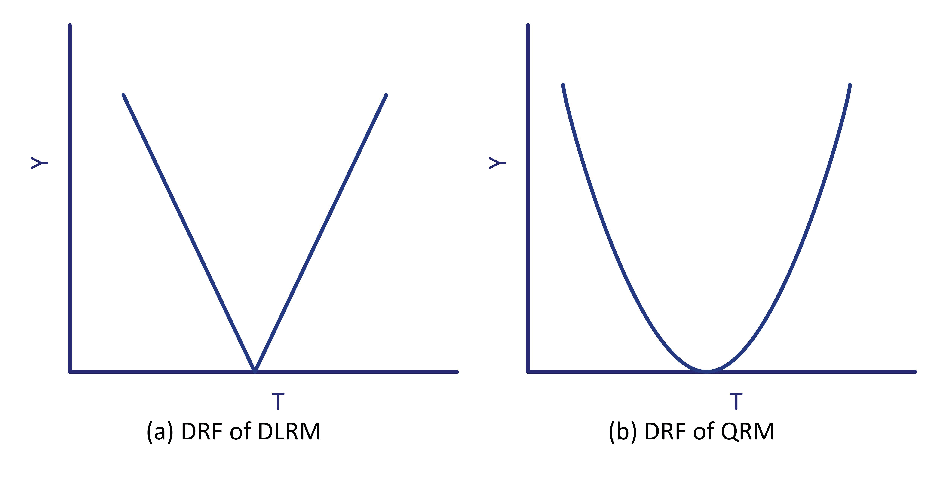
\includegraphics[width=0.7\textwidth]{DRF_curves.eps}
\caption{Matching units based on their propensity scores breaks the link between cofounding variables and treatment.}
%\vspace{-.5cm}
\label{DRF_curves}
\end{figure*}
\vspace{-0.1cm}

Finally, we chose to use the absolute value of fitted a regression coefficient's $t$-statistic [19] as a suspiciousness score, rather than the coefficient itself, because we wish to ``penalize" coefficients with large standard errors.  We use $\left| t \right|$ to denote the absolute value of the $t$-statistic for a fitted coefficient $\hat \beta $: $\left| t \right| = |\hat \beta /std ( {\hat \beta })|$ , where $std(\hat \beta)$ is the standard error of $\hat \beta$.  Thus, for DLRM the failure-causing effect of treatment $T_e$ is estimated by the summation of two linear regression models'$\left| t \right|$ values for the fitted slope coefficient ${{\hat \gamma }_e}$.  For QRM, this effect is estimated by the $\left| t \right|$ value of the estimated coefficient ${\hat \zeta }$ of the quadratic term of the regression model.

\renewcommand{\algorithmicrequire}{\textbf{Input:}}
\renewcommand{\algorithmicensure}{\textbf{Output:}}
\begin{algorithm}
  \captionof{figure}{ {\it NUMFL} Algorithm}\label{NUMFLalg}

  \begin{algorithmic}[1]
    \Require Subexpression value table $E=[T_e, \pmb{X}_e]$, with all values standardized, and type of model $M$
    \Ensure Suspiciousness scores $\tau \left( e \right)$ of subexpressions, sorted in descending order
    \For  {each subexpression $e$ }
        \State        $T_e \gets$ treatment variable of {\it i}th subexpression
        \State        $\pmb{X}_e\gets$ confounding variables of {\it i}th subexpression
        \If{ using GPS}
            \State Fit linear regression model ${T_e} = {\pmb{X}_e}'{\pmb{\beta} _e}$
        \ElsIf{using CBPS}
            \State Fit models for $Pr(T_e=k \mid \pmb{X}_e)$,
            \State$k = 1 \ldots K$, using multinomial logistic regression
        \EndIf
        \For  {each  ${\pmb{x}_{e,j}}$ }
            \State Estimate the propensity score for ${\pmb{x}_{e,j}}$ using fitted GPS or
            \State CBPS model(s).
        \EndFor
        \State Group the observations into $m$ roughly equal-size subclasses.
        \For  {each subclass $k$ }
            \If{ $M$ is DLRM }
                 \State Fit two linear regression models:
                 \State  $Y = {\gamma _{e,1}}{T_e} + b$   for observations $T_e>median(T_e)$
                 \State  $Y = {\gamma _{e,2}}{T_e} + b$   for observations $T_e \le median(T_e)$
                 \State  ${\tau _1} = t$-value of ${\gamma _{e,1}}$
                 \State  ${\tau _2} = t$-value of ${\gamma _{e,2}}$
                 \State ${\tau ^k} = |{\tau _1}| + |{\tau _2}|$
            \EndIf
            \If{$M$ is QRM}
                \State Fit quadratic regression model $Y = \zeta {T_e}^2 + \eta {T_e} + c$
                \State ${\tau ^k} = |t$-value of $\hat \zeta |$
            \EndIf
        \EndFor
        \State $\tau(e)$ = weighted average of  $\tau^k$ across $m$ subclasses
    \EndFor
    \State Sort  $\tau(e)$ values in descending order.

  \end{algorithmic}
\end{algorithm}


Figure \ref{NUMFLalg} shows the NUMFL-GPS algorithm.  Note that all input values are standardized $(x \to \frac{{x - \mu }}{\sigma })$ to adjust for differences in scale between variables.  NUMFL-GPS processes each numeric expression or subexpression e in three stages.  In the first stage (lines 2-5 and 10-14), it fits a linear propensity score model regressing the treatment variable $T_e$ on the confounding variables $X_e$, then uses the fitted model to calculate the generalized propensity score for each observation.  The scores are grouped into $m$ roughly equal-sized subclasses.  In the second stage (lines 15-28), the algorithm estimates the ``penalized" AFCE of $T_e$ on $Y$ separately in each subclass.  If DLRM is employed, the data within a subclass is split into two equal-size groups.  The algorithm fits a linear model for each group, and it records the {\it t}-statistics ${\tau _1}$ and ${\tau _2}$ for the coefficients of $T_e$ in the two models.  The penalized AFCE for subclass $k$ is given by the sum ${\tau ^k} = |{\tau _1}| + \left| {{\tau _2}} \right|$.  If QRM is employed, the algorithm fits a quadratic model and records the coefficient ${\hat \zeta }$ of the quadratic term.  The penalized AFCE for subclass $k$ is estimated by the absolute value of the {\it t}-statistic for ${\hat \zeta }$.  In the third stage, the overall AFCE or suspiciousness score $\tau(e)$ for subexpression $e$ is computed as a weighted average of $\tau^k$ over all subclasses $k$ (line 29).  Finally, the suspiciousness scores for all subexpressions are sorted in descending order (line 31).  The developer uses the sorted list to guide fault localization.

\subsection{NUMFL-CBPS}\label{IVB}
NUMFL-CPBS differs from NUMFL-GPS in that the former employs the Covariate Balancing Propensity Score instead of GPS for confounding control.   Recall from Section \ref{IIID} that the CBPS seeks to optimize covariate balance by employing the Generalized Method of Moments (GMM), which solves balance equations for the parameters of interest.

\subsubsection{Control of Confounding.}
In Imai and Ratkovic's extension of CBPS to treatment variables with $K>2$ discrete values \cite{Hansen1982}, a multinominal logistic regression model is used to estimate the conditional probability $\pi_{\pmb \beta}^k (\pmb{x})=Pr(T=k \mid \pmb{X})$ of treatment $k$. To handle a continuous treatment variable $T_e$ associated with a numerical expression $e$, we discretize the values of $T_e$ by partitioning them into ordered bins.  For each $k$, $1 \leq k<K$, the probability  that the original value of $T_e$ belongs in bin $k$ is modeled by
\begin{equation*}
\Pr ({T_e} = k \mid{\pmb{X}_e}) = \frac{{{e^{{{\pmb \beta} _k}{\pmb{x}_e}}}}}{{1 + \sum\nolimits_{i = 1}^{K - 1} {{e^{{{\pmb \beta} _i}{\pmb{x}_e}}}} }}
\end{equation*}
and
\begin{equation*}
\Pr ({T_e} = K\mid{\pmb{X}_e}) = \frac{1}{{1 + \sum\nolimits_{i = 1}^{K - 1} {{e^{{{\pmb \beta} _i}{\pmb{x}_e}}}} }}
\end{equation*}
The CBPS can be estimated using the open source R package ``CBPS" created by Fong, {\it et al} \cite{CBPS}.

The whole process of applying CBPS in NUMFL involves the following three steps:
\begin{enumerate}
\item 	Given a sample of observed values for the discretized treatment variable $T_e$ and for the covariates $\pmb{X}_e$, use the R package ``CBPS" to estimate the coefficients of a multinominal logistic propensity score model $\pi _{\pmb{\beta}} ^k({\pmb{x}_{e,i}}) = P({T_{e,i}} = k \mid {\pmb{x}_{e,i}})$ for each $k$.
\item	For each observed value ${\pmb x}_{e,i}$, estimate propensity score $\hat \pi _{e,i}$ with the fitted propensity score model.
\item Group observations with the same or similar values of $\hat \pi _{e,i}$ into $m$ subclasses of roughly equal size.
\end{enumerate}

Here $\hat \pi _{e,i}$ represents the calculated propensity score for each observed value.  Similar $\hat \pi _{e,i}$ values correspond to a set of $\pmb{x}_{e,i}$ values that influence the treatment similarly, so we group the observations into subclasses as we did in NUMFL-GPS.  Propensity score estimation and grouping in NUMFL-CBPS corresponds to lines 6-14 in the algorithm of Figure \ref{NUMFLalg}.

\subsubsection{Failure-causing Effect Estimation.}
Failure-causing-effect estimation in NUMFL-CBPS follows the same process followed in NUMFL-GPS, which is shown in lines 15-29 of Figure \ref{NUMFLalg}.  For a given subexpression $e$, QRM or DLRM is used to estimate the ``penalized" AFCE of $T_e$ on $Y$ within each subclass individually. Then the failure-causing effect is calculated as a weighted average the penalized AFCEs over all subclasses. Finally, the results for all subexpressions are sorted.

\begin{table*}[htbp!]
\caption{STANDARDIZED VARIABLE VALUES OF THE MOTIVATING EXAMPLE}
\label{exampledata2}
\centering
      \begin{tabular}{|l|c|c|c|c|c|c|c|c|c|c|}
      \hline
Test \#	&	1	&	2	&	3	&	4	&	5	&	6	&	7	&	8	&	9	&	10	\\	\hline
$a$	&	-0.166	&	0.876	&	0.183	&	0.091	&	-0.490	&	-0.235	&	-0.232	&	-0.382	&	0.831	&	-0.475	\\	\hline
$b$	&	-0.364	&	0.023	&	0.797	&	-0.433	&	-0.720	&	0.138	&	-0.381	&	0.746	&	0.233	&	-0.039	\\	\hline
$c$	&	-0.523	&	0.834	&	-0.218	&	0.113	&	-0.119	&	0.111	&	0.832	&	-0.646	&	-0.269	&	-0.114	\\	\hline
$k$	&	-0.336	&	0.580	&	0.619	&	-0.213	&	-0.769	&	-0.065	&	-0.389	&	0.222	&	0.683	&	-0.331	\\	\hline
$x$	&	-0.110	&	0.404	&	-0.079	&	-0.001	&	0.631	&	-0.204	&	0.431	&	-1.156	&	0.269	&	-0.186	\\	\hline
$r$	&	-0.027	&	0.517	&	0.358	&	-0.031	&	-0.460	&	0.478	&	-0.328	&	-1.027	&	0.501	&	0.020	\\	\hline
$Y$	&	2.552	&	1.592	&	0.882	&	0.335	&	0.490	&	0.896	&	2.102	&	5.611	&	0.900	&	1.065	\\	\hline
\end{tabular}
\end{table*}

We will use the expression $s_3$ and $s_8$ in the faulty code of motivating example shown in Figure\ref{code} to  demonstrate the NUMFL algorithm in Figure\ref{NUMFLalg} step by step. The variable values are come from  Table\ref{exampledata}. In the motivating example, we know that the bug exists in expression $s_3$, so the estimated suspiciousness score of $s_3$ should be larger than the estimated suspiciousness score of $s_8$. In practice, running the NUMFL algorithm requires decomposing complex numerical expression in to several subexpressons , which has relatively simple structure. But the expressions $s_3$ and $s_8$ already have simple structure, so we choose to estimate the AFCE of the expressions without decomposing them into subexpressions. 

For expression $s3$ , the first step is to identify the treatment variable and confounding variables. In the expression $s3$, the treatment variable $T_e$ is variable $x$ and the confounding variables are $a$, $b$ and $c$. Then we adjust  the differences in scale between variables by standardizing the variables' values. Table\ref{exampledata2} shows all the variables values after standardization. Note that the outcome variable $Y$ is not standardized. Next we estimate propensity scores for each observations. To estimate GPS ${\hat{\theta}}_{s_3}$, we can fit a linear regression model as described in section\ref{IIIC}. If NUMFL-CBPS is used, we need to fit a multinomial logistic regression model, which is some what complex. Here we use R package "CBPS" to estimate the CBPS which can automatically fit a multinomial regression model with the treatment variables and confounding variables and then estimate the propensity score. For the detail of the package "CBPS", the reader should refer to \cite{CBPS}. Table\ref{exampledata3} shows expression $s_3$'s  estimated GPS ${\hat{\theta}}_{s_3}$ and CBPS ${\hat{\pi}}_{s_3}$ for each observation. With the estimated propensity scores, we group observations with same or similar propensity scores into $m$ subclasses. For simplicity, we use $m=2$ for the motivating example. We rank the tests according to their propensity scores in descending order. The first 5 tests are in subclass 1 and the last 5 tests are in subclass 2. The last two columns of Table\ref{exampledata3} shows the subclass index of each test for NUMFL-GPS and NUMFL-CBPS. From Table\ref{exampledata3}, we can see there is some difference between the subclassification results of NUMFL-GPS and NUMFL-CBPS. In NUMFL-GPS, test 4 and test5 are in subclass 2 , while in NUMFL-CBPS, test4 and test5 belong to subclass1.  Similarly, we calculate GPS and CBPS for expression $s_8$, which is summarized in Table\ref{exampledata4}.  

The suspiciousness score of expression is estimated by the average of failure-causing effect in two subclasses. Assume we use QRM to estimate failure-causing effect,  a quadratic regression model $Y = \zeta {T_e}^2 + \eta {T_e} + c$  is fitted in each subclass. The $|t$-value$|$ of  the coefficient $\zeta$ is the estimated failure-causing effect. Table\ref{exampledata5} shows the estimated failure-causing effect in each subclass when NUMFL-GPS is used.  In Table\ref{exampledata5},  ${|t-value|}_1$ denotes the estimated failure-causing effect in subclass1 and ${|t-value|}_2$ denotes the estimated failure-causing effect in subclass2. The estimated suspiciousness score (AFCE) is equal to  $({{|t-value|}_1}+{{|t-value|}_2})/2$. For comparison, we also fit a quadratic regression model with full sample without subclassification and the estimated failure-causing effect is denoted by ${|t-value|}_0$. In Table\ref{exampledata5}, ${|t-value|}_0$ of $s_8$ is close to ${|t-value|}_0$ of $s_3$, even though $s_8$ is not faulty. This is because the faulty variable $x$ in $s_3$ is confounder of variable $r$ in  $s_8$ and make $s_8$ associate to program failure. When NUMFL-GPS is applied, the estimated AFCE of $s_8$ is significantly smaller than the estimated AFCE of $s_3$. The estimated suspiciousness scores of NUMFL-CBPS are shown in  Table\ref{exampledata6}. In Table\ref{exampledata6}, the difference between  $s_3$ and $s_8$'s suspiciousness score is larger than the difference between their ${|t-value|}_0$s. This means both GPS and CBPS are effective in controlling confounding bias.  


\begin{table*}[htbp!]
\caption{ESTIMATED GPS AND CBPS OF EXPRESSION $s_3$}
\label{exampledata3}
\centering
      \begin{tabular}{|l|c|c|c|c|}
      \hline
Test \#	&	${\hat{\theta}}_{s_3}$	&	${\hat{\pi}}_{s_3}$	&	Subclass index (GPS)	&	Subclass index (CBPS)	\\ \hline
1	&	0.057	&	0.847	&	2	&	2	\\ \hline
2	&	0.364	&	0.716	&	2	&	2	\\ \hline
3	&	-0.606	&	5.65E-11	&	1	&	1	\\ \hline
4	&	0.310	&	5.05E-06	&	2	&	1	\\ \hline
5	&	0.692	&	1.60E-09	&	2	&	1	\\ \hline
6	&	-0.143	&	5.872	&	1	&	2	\\ \hline
7	&	0.637	&	2.570	&	2	&	2	\\ \hline
8	&	-1.119	&	5.22E-06	&	1	&	1	\\ \hline
9	&	-0.113	&	0.130	&	1	&	1	\\ \hline
10	&	-0.079	&	5.694	&	1	&	2	\\ \hline
\end{tabular}
\end{table*}

\begin{table*}[htbp!]
\caption{ESTIMATED GPS AND CBPS OF EXPRESSION $s_8$}
\label{exampledata4}
\centering
      \begin{tabular}{|l|c|c|c|c|}
      \hline
Test \#	&	${\hat{\theta}}_{s_8}$	&	${\hat{\pi}}_{s_8}$	&	Subclass index (GPS)	&	Subclass index (CBPS)	\\ \hline
1	&	-0.258	&	0.521	&	1	&	2	\\ \hline
2	&	0.562	&	3.156	&	2	&	2	\\ \hline
3	&	0.323	&	3.878	&	2	&	2	\\ \hline
4	&	-0.127	&	3.099	&	1	&	2	\\ \hline
5	&	-0.110	&	0.004	&	2	&	1	\\ \hline
6	&	-0.149	&	1.14E-07	&	1	&	1	\\ \hline
7	&	0.005	&	0.008	&	2	&	1	\\ \hline
8	&	-0.498	&	1.51E-06	&	1	&	1	\\ \hline
9	&	0.549	&	3.079	&	2	&	2	\\ \hline
10	&	-0.297	&	0.069	&	1	&	1	\\ \hline
\end{tabular}
\end{table*}

\begin{table*}[htbp!]
\caption{ESTIMATED AFCE WITH NUMFL-GPS}
\label{exampledata5}
\centering
      \begin{tabular}{|l|c|c|c|c|}
      \hline
Expression& ${|t-value|}_1$  & ${|t-value|}_2$ & Suspiciousness score & ${|t-value|}_0$\\	\hline

$s_3$ &  13.861 &0.228 &7.045 &2.763 \\	\hline
$s_8$& 1.045 &0.515 &0.78 &2.601\\	\hline
\end{tabular}
\end{table*}

\begin{table*}[htbp!]
\caption{ESTIMATED AFCE WITH NUMFL-CBPS}
\label{exampledata6}
\centering
      \begin{tabular}{|l|c|c|c|c|}
      \hline
Expression& ${|t-value|}_1$  & ${|t-value|}_2$  & Suspiciousness score & ${|t-value|}_0$\\	\hline
$s_3$ &  4.034 &2.219 &3.127 &2.763\\	\hline
$s_8$& 1.898&0.325 &1.112 &2.601\\	\hline
\end{tabular}
\end{table*}

\section{EMPIRICAL EVALUATION}\label{evaluation}
To evaluate the effectiveness of NUMFL, we conducted an empirical study involving several subject programs, in which the performance of NUMFL was compared with the performance of several baselines techniques. In the study, we investigated four main research questions:  (1) What is the performance of NUMFL compare to baseline techniques when each subject program version contains only one fault?  (2) What is the performance of NUMFL compare to the baselines when each subject program version contains two faults?   (3) Given data from only failing executions, is NUMFL effective?  (4) Which is most effective, NUMFL-GPS or NUMFL-CBPS?

\subsection{Experimental Platform and Data Collection}
We developed a data collection and analysis platform for numerical fault localization studies involving Java programs.  The platform is based on a modified Java parser \cite{Java} and the ASM Java bytecode manipulation framework \cite{ASM}.  We first parse the source code of a subject program.  Each complete numerical expression is decomposed into a set of subexpressions as described in Section \ref{IVA}.  The ASM compiler is used to instrument the bytecode files of the subject program to record variable values used and produced by the evaluation of each subexpression.  Information is recorded to permit the recorded values to be mapped back to the corresponding source-code subexpressions.  Each instrumented subject program is executed on a test suite and the induced variable values are recorded.  For a subexpression within a loop, we currently record the associated values only for the last iteration of the loop, in order to reduce overhead.

The data collection algorithm is implemented in Java and can be downloaded from \cite{NUMFL}.  The NUMFL algorithm and other baseline techniques were implemented using the R statistical computing environment \cite{R}. In this study, the number of propensity score subclasses used in the NUMFL algorithm was set to 10.

\subsection{Subject Programs, Faults, and Tests}
{\bf Subject Programs.}  For the empirical study, we selected 16 subject programs from four Java numerical libraries: (1) Apache Common Math (versions 2.1 and 3.1.1), which is a popular Java library for scientific computing \cite{Commons}; (2) the Oj! Algorithms library Ojalgo (version 33.0), which is an open source Java library for mathematics, linear algebra and optimization \cite{Oj}; (3) JAMA, which is a basic linear algebra package for Java \cite{JAMA}; and (4) SciMark 2.0, which is a Java benchmark for measuring the performance of numerical codes occurring in scientific applications \cite{SciMark}.  We chose subject programs whose purpose we understood (so that we would be able to write tests for them if necessary) and having as many numerical expressions as possible.  We chose four large ($\ge 1500$ SLOC) and eight small subject programs ($< 1500$ SLOC) from Apache Common Math; for Ojalgo, we wrote a subject program to calculate the Schur decomposition of a matrix that uses two Ojalgo classes (PrimitiveDenseStore and HermitianEVD32); for JAMA, we created one subject program that uses four different matrix decomposition algorithms; we used two of SciMark's five computation kernels as subject programs, FFT and LU factorization.  A summary of our subject programs is shown in Table \ref{subpro}.

\begin{table*}[htbp!]
\caption{SUMMARY OF SUBJECT PROGRAMS}
\label{subpro}
      \begin{tabular}{|l|c|c|c|c|}
      \hline
Subject Program	&	SLOC	&	\# of Sub-expressions	&	\# of Tests	&	\# Faulty versions	\\	\hline
Apache\_EigenDecompose	&	1858	&	611	&	8000	&	10	\\	\hline
Apache\_DScompiler	&	1774	&	220	&	5000	&	10	\\	\hline
Apache\_BigMatrix	&	1580	&	244	&	3000	&	10	\\	\hline
Apache\_Rotation3D	&	1704	&	504	&	3000	&	10	\\	\hline
Ojaljo\_SchurDecompose	&	2129	&	649	&	5000	&	10	\\	\hline
Jama\_MatrixDecompose	&	1952	&	578	&	5000	&	10	\\	\hline
SciMark\_LU	&	295	&	35	&	3000	&	2	\\	\hline
SciMart\_FFT	&	197	&	59	&	3000	&	2	\\	\hline
Apache\_SymmLQ	&	1226	&	57	&	5000	&	2	\\	\hline
Apache\_SplineInterpolator	&	130	&	45	&	5000	&	2	\\	\hline
Apche\_SimpleRegress	&	869	&	61	&	5000	&	2	\\	\hline
Apache\_SchurTransformer	&	458	&	154	&	3000	&	2	\\	\hline
Apache\_MillerUpdatRegress	&	1110	&	152	&	1000	&	2	\\	\hline
Apache\_HarmonicFitter	&	385	&	50	&	3000	&	2	\\	\hline
Apache\_FastSine	&	197	&	66	&	5000	&	2	\\	\hline
Apache\_FastCosine	&	188	&	77	&	5000	&	2	\\	\hline
\end{tabular}
\end{table*}

{\bf Faults.}  To evaluate NUMFL, we required faulty versions of subject programs.  After much searching, we were able to find few well documented faults (including fixes) that produced numerical output that was sometimes, but not always, incorrect.  Hence, we {\it injected} three types of simulated numerical faults into the subject programs: (1) adding a small random number to a numerical expression (the number varied between and within runs); (2) multiplying a numerical expression by a random number; (3) randomly changing one of the operators of a numerical expression (once only).  Each faulty version of a subject program contained one bug.  We generated 12 faulty versions of each subject program whose number of lines of source code was larger than 1500.  For each subject program with fewer than 1500 SLOC, we generated two faulty versions.  Except for SciMark, every subject program came with a unit test suite which provided a predefined error tolerance; we chose a tolerance of 1.0E-5 for SciMark.  We ran the faulty versions of the subject programs and the original correct versions with the same inputs.  If the output error $Y$ exceeded the tolerance, the execution was considered to be failure.  If the subject program's output was a scalar variable, the output error $Y$ was the absolute difference between the correct and faulty programs' outputs.  If the subject program's output was an array, we calculated the difference between each element in the faulty program's output and the corresponding element in correct program's output.  The output error $Y$ was taken to be the first difference encountered that was larger than the tolerance or zero if no such difference was found.


{\bf Tests.}  Since a number of our subject programs came with very few test cases, it was necessary to create test cases for them.  We first analyzed the subject programs and the test cases provided by their developers. Then we randomly generated inputs similar to those of the test cases. Note that for NUMFL, we did not generally use the total number of tests shown in Table \ref{subpro}, though we did so for the baseline techniques.  Instead, we first selected all $N$ tests of the smaller of the set of failed tests and the set of passed tests, and we then randomly selected $N$ tests from the larger set. (See Section \ref{VE} for an exception.)

\subsection{Baseline SFL Metrics and Cost Measure}

{\bf Baselines.}  We compared NUMFL to four baseline SFL metrics.  Two are coverage-based metrics that have performed well in comparisons with other such metrics: Ochiai \cite{Abreu2007} and DStar (with $star = 2$) \cite{Wong2014}.   The Ochiai metric estimates the suspiciousness of a statements $s$ with the equation
\begin{equation}
O(s) = {f_s}/\sqrt {f({f_s} + {p_s})}
\end{equation}
where: $f_s$ is the number of failed tests that cover statement $s$; $p_s$ is number of passed tests that cover $s$; and $f$ is the total number of failed tests.  The Dstar metric (with $star = 2$) is
\begin{equation}
D(s) = {f_s}^2/({p_s} + f - {f_s})
\end{equation}
where $f-f_s$ is the number of failed tests that do not cover $s$.

The other two baselines are predicate-level SFL metrics, SOBER \cite{Liu2005} and the Exploratory Software Predictor (ESP) \cite{Gore2011}.  SOBER computes the probability $\pi(P)$ that a predicate $P$ evaluated to be true in an execution.  If the distribution of $\pi(P)$ in passing runs differs significantly from its distribution in failing runs then $P$ is considered to be related to the fault.  In this study, for a treatment variable $T_e$ we use these predicates [20]: $T_e>0$, $T_e=0$ and $T_e<0$.

ESP employs ``elastic predicates" to partition the value space for each variable $x$ at each assignment to $x$.  ESP provides two instrumentation schemes: single variable and scalar pairs.  The single variable scheme uses execution profiles to compute the mean $\mu_x$ and standard deviation $\sigma_x$ for a variable $x$.  These statistics are then used in nine predicates (e.g., $x<\mu_x+\sigma_x$) that collectively partition the values of $x$ for three standard deviations above and below $\mu_x$.  ESP then computes an importance score for each predicate.  The suspiciousness of each assignment to $x$ is taken to be the highest importance score among the corresponding elastic predicates.  In a similar way, the scalar pair [31] scheme addresses differences in the values of pairs of variables (e.g.,  $x-y>\mu_{x-y}+\sigma_{x-y}$).

{\bf Cost Measure.}  We measured the costs of applying NUMFL and the baseline metrics by the percentage of {\it subexpressions} that need to be examined, in decreasing order of suspiciousness scores, to find the fault, assuming the fault is recognized when it is encountered.  This contrasts with most SFL techniques, which localize faults at the statement level.  There are two reasons that we chose to have NUMFL compute suspiciousness scores for subexpressions rather than for statements.  First, the location of a faulty subexpression not only implies the location of the numerical statement that contains the subexpression, but it also indicates which part of the statement is problematic.   Second, in this study we collected data only for floating point variables involved in numerical expressions.   As a result, the number of subexpressions was usually smaller than the number of lines of code.  To ensure a fair comparison between NUMFL and the predicate-level baseline metrics, predicates were associated with subexpressions.  In comparing NUMFL to the statement-level, coverage-based baseline metrics, subexpressions belonging to same statement received the {\it same suspiciousness score}.   To compare NUMFL fairly to the latter metrics, if multiple subexpressions got the same suspiciousness score as the faulty subexpression, we considered the faulty subexpression to rank in the middle of them.

\subsection{Comparative Performance of NUMFL vs. Baselines}\label{VD}
Table \ref{table2} shows, for NUMFL-GPS and the baseline metrics and for each subject program, the average percentage of subexpressions that had to be examined to find the fault, computed across all the faulty versions.  Here we show the results for QRM but not for DLRM, which QRM outperformed.  (Nevertheless, DLRM outperformed the 5 baseline metrics.)  For 14 of 16 subject programs, NUMFL-GPS-QRM performed better than Ochiai, DStar ($star=2$), and SOBER. NUMFL-GPS-QRM performed better than ESP-SIV (single variable) and ESP-SCP (scalar pair) for all 16 subject programs.  Overall, NUMFL-GPS-QRM was more effective in localizing numerical faults than any of the baseline metrics.
\begin{table*}[htbp!]
\fontsize{8pt}{9pt}\selectfont
\centering
\caption{AVERAGE FAULT LOCALIZATION COSTS OF NUMFL-GPS-QRM AND BASELINE METRICS ON SINGLE-FAULT PROGRAM VERSIONS}
\label{table2}
      \begin{tabular}{|l|c|c|c|c|c|c|}
      \hline
\multirow{2}{*}{{\bf Subject Program}}	&	\multicolumn{6}{|c|}{{\bf Technique}}	\\	\cline{2-7}
&{NUMFL-GPS-QRM}	&{ Ochiai}&	{ Dstar}&	{ ESP(SIV)} &	{ ESP(SCP)}	&{SOBER} \\\hline
Apache\_EigenDecompose	&	12.3\%	&	9.2\%	&	9\%	&	22.2\%	&	17.2\%	&	7.8\%	\\	\hline
Apache\_DScompiler	&	11\%	&	19.9\%	&	16.5\%	&	22.9\%	&	18.9\%	&	24.2\%	\\	\hline
Apache\_BigMatrix	&	11.4\%	&	51.8\%	&	51.8\%	&	37.9\%	&	31.8\%	&	28.9\%	\\	\hline
Apache\_Rotation3D	&	8\%	&	30.5\%	&	30.5\%	&	20.1\%	&	23.6\%	&	28.5\%	\\	\hline
Ojaljo\_SchurDecompose	&	11.4\%	&	22.7\%	&	22.7\%	&	20.2\%	&	27.3\%	&	30.9\%	\\	\hline
Jama\_MatrixDecompose	&	14.2\%	&	11.4\%	&	11.4\%	&	24.3\%	&	27\%	&	46.4\%	\\	\hline
SciMark\_LU	&	15.3\%	&	38.9\%	&	68.1\%	&	27.8\%	&	18.8\%	&	12.5\%	\\	\hline
SciMart\_FFT	&	9.5\%	&	48.3\%	&	75\%	&	68.1\%	&	36.6\%	&	12.5\%	\\	\hline
Apache\_SymmLQ	&	2.6\%	&	37.7\%	&	85.1\%	&	7\%	&	10.5\%	&	32.9\%	\\	\hline
Apache\_SplineInterpolator	&	31.7\%	&	51.1\%	&	47.8\%	&	65\%	&	64.4\%	&	56.1\%	\\	\hline
Apche\_SimpleRegress	&	4.3\%	&	49.2\%	&	29.9\%	&	7.3\%	&	7.2\%	&	7.9\%	\\	\hline
Apache\_SchurTransformer	&	3.3\%	&	8.2\%	&	8.2\%	&	36.2\%	&	10.2\%	&	44.4\%	\\	\hline
Apache\_MillerUpdatRegress	&	7.5\%	&	12.7\%	&	12.7\%	&	37.6\%	&	19.6\%	&	14.5\%	\\	\hline
Apache\_HarmonicFitter	&	27.3\%	&	45\%	&	58.5\%	&	39.5\%	&	41.7\%	&	49.3\%	\\	\hline
Apache\_FastSine	&	1.5\%	&	30.2\%	&	87.1\%	&	41.9\%	&	3.8\%	&	26.7\%	\\	\hline
Apache\_FastCosine	&	1.3\%	&	33.2\%	&	94.9\%	&	79.7\%	&	41.4\%	&	31.2\%	\\	\hline
Average Cost	&	10.8\%	&	31.3\%	&	44.3\%	&	34.9\%	&	25\%	&	28.4\%	\\	\hline
\end{tabular}
\end{table*}


We also compare the performance of NUMFL-GPS-QRM to that of each baseline SFL metric graphically. The comparison measure is the difference between the cost for the baseline metric and the cost for NUMFL-GPS-QRM.  Since the two costs are percentages, the difference is the percentage reduction in cost obtained by using NUMFL-GPS-QRM, which may be positive or negative.  For example, if the cost of using NUMFL-GPS-QRM is 10\% and the cost of using the baseline metric is 40\%, then the improvement is 30\%.  Figure \ref{QRM_VS_Base} shows the results of comparisons of NUMFL-GPS-QRM with each of the baseline metrics.  In each graph, the vertical axis represents the percentage improvement (reduction) in cost. The horizontal-axis represents different subject-program versions for which there are cost differences between the metrics, with each version represented by a vertical bar.   Bars above the zero-line represent versions for which NUMFL-GPS-QRM performed better than the baseline metric and bars below zero represent versions for which NUMFL-GPS-QRM performed worse.  The length of each bar represents the magnitude of the corresponding cost difference.

\textit{\textbf{ NUMFL-GPS-QRM vs. Ochiai.}}  Over all 92 faulty subject-program versions, NUMFL-GPS-QRM performed better than the Ochiai metric on 67 versions but NUMFL-GPS-QRM performed worse on 25 versions.  There were 38 versions for which NUMFL-GPS-QRM performed at least 20\% better than the Ochiai metric.  There were just 5 versions for which the latter performed better than NUMFL-GPS-QRM.

\textit{\textbf{ NUMFL-GPS-QRM vs. DStar.}}  NUMFL-GPS-QRM performed better than DStar on 70 subject-program versions but NUMFL-GPS-QRM performed worse than DStar on 22 versions.  NUMFL-GPS-QRM performed at least 20\% better than DStar on 42 versions, whereas DStar performed at least 20\% better than NUMFL-GPS-QRM on just 5 versions.

\textit{\textbf{ NUMFL-GPS-QRM vs. ESP-SIV.}} NUMFL-GPS-QRM performed better than ESP-SIV on 70 subject-program versions but NUMFL-GPS-QRM performed worse than ESP-SIV on 22 versions.  NUMFL-GPS-QRM performed at least 20\% better than ESP-SIV on 31 versions, whereas ESP-SIV performed at least 20\% better than NUMFL-GPS-QRM on just 5 versions.

\textit{\textbf{ QRM vs. ESP-SCP.}}  NUMFL-GPS-QRM performed better than ESP-SCP on 61 subject-program versions but NUMFL-GPS-QRM performed worse than ESP-SCP on 31 versions.  NUMFL-GPS-QRM performed at least 20\% better than ESP-SIV on 27 versions, whereas ESP-SCP performed at least 20\% better than NUMFL-GPS-QRM on just 3 versions.

\textit{\textbf{ QRM vs. SOBER.}}  NUMFL-GPS-QRM performed better than SOBER on 64 subject-program versions but NUMFL-GPS-QRM performed worse than SOBER on 28 versions.  NUMFL-GPS-QRM performed at least 20\% better than SOBER on 32 versions, whereas SOBER performed at least 20\% better than NUMFL-GPS-QRM on just 7 versions.

% figure example
%\begin{landscape}
\begin{sidewaysfigure}
\centering
\includegraphics[width=\textwidth]{QRM_VS_Base.eps}
\caption{Performance of NUMFL-GPS-QRM relative to baseline metrics on individual single-fault program versions.}
\label{QRM_VS_Base}
\end{sidewaysfigure}
%\end{landscape}

\subsection{NUMFL-GPS Applied only to Failing Runs}\label{VE}
Conventional, coverage-based and predicate-based SFL techniques require profiles and PASS/FAIL labels from both passing and failing runs, in order to rank statements based on estimates of quantities like $Pr [failure \mid s covered]$ \cite{Baah2010} that vary between statements only if the data come from a mix of passing and failing runs.  However, because many numerical programs have few conditional branches, a particular fault may be executed and cause erroneous values to occur on every run that is observed.  If these values propagate to the program output, a failure may occur on every run, depending on the numerical accuracy required.


Even if it is applied to data from only failing runs, NUMFL can still produce different AFCE estimates for different statements, because the causal outcome of interest is a continuous variable--the output error of a numerical program.  To evaluate whether NUMFL-GPS is actually effective when it is applied to data from only failing runs, we redid the study just described, after creating a new data set by removing the data from passing runs.  Table \ref{table3} and Figure \ref{QRM_allFail} compare the performance of QRM with such data to its performance with the original data from both passing and failing runs.  Figure \ref{QRM_allFail} shows that over all 92 faulty subject-programs versions, QRM performed better with data from only failing runs on 43 program versions and it performed worse on 49 versions.  There were only 8 versions for which QRM performed at least 20\% worse with data from only failing runs.

\begin{table*}[htbp!]
\caption{AVERAGE FAULT LOCALIZATION COSTS OF NUMFL-GPS-QRM WITH AND WITHOUT DATA FROM PASSING RUNS, ON SINGLE-FAULT PROGRAM VERSIONS}
\label{table3}
\centering
      \begin{tabular}{|l|c|c|}
      \hline
\multirow{2}{*}{{\bf Subject Program}}	&	\multicolumn{2}{|c|}{{\bf Input}}	\\	\cline{2-3}
& Pass and Fail	&Fail only \\ \hline
Apache\_EigenDecompose	&	12.3\%	&	11.4\%	\\	\hline
Apache\_DScompiler	&	11\%	&	11\%	\\	\hline
Apache\_BigMatrix	&	11.4\%	&	8\%	\\	\hline
Apache\_Rotation3D	&	8\%	&	18.9\%	\\	\hline
Ojaljo\_SchurDecompose	&	11.4\%	&	17.7\%	\\	\hline
Jama\_MatrixDecompose	&	14.2\%	&	24.5\%	\\	\hline
SciMark\_LU	&	15.3\%	&	54.1\%	\\	\hline
SciMart\_FFT	&	9.5\%	&	17.2\%	\\	\hline
Apache\_SymmLQ	&	2.6\%	&	2.6\%	\\	\hline
Apache\_SplineInterpolator	&	31.7\%	&	21.7\%	\\	\hline
Apche\_SimpleRegress	&	4.3\%	&	3.4\%	\\	\hline
Apache\_SchurTransformer	&	3.3\%	&	8.2\%	\\	\hline
Apache\_MillerUpdatRegress	&	7.5\%	&	12.7\%	\\	\hline
Apache\_HarmonicFitter	&	27.3\%	&	47.5\%	\\	\hline
Apache\_FastSine	&	1.5\%	&	1.5\%	\\	\hline
Apache\_FastCosine	&	1.3\%	&	1.3\%	\\	\hline
Average Cost	&	10.8\%	&	16.4\%	\\	\hline
\end{tabular}
\end{table*}

% figure example
\begin{figure*}[!thpb]
\centering
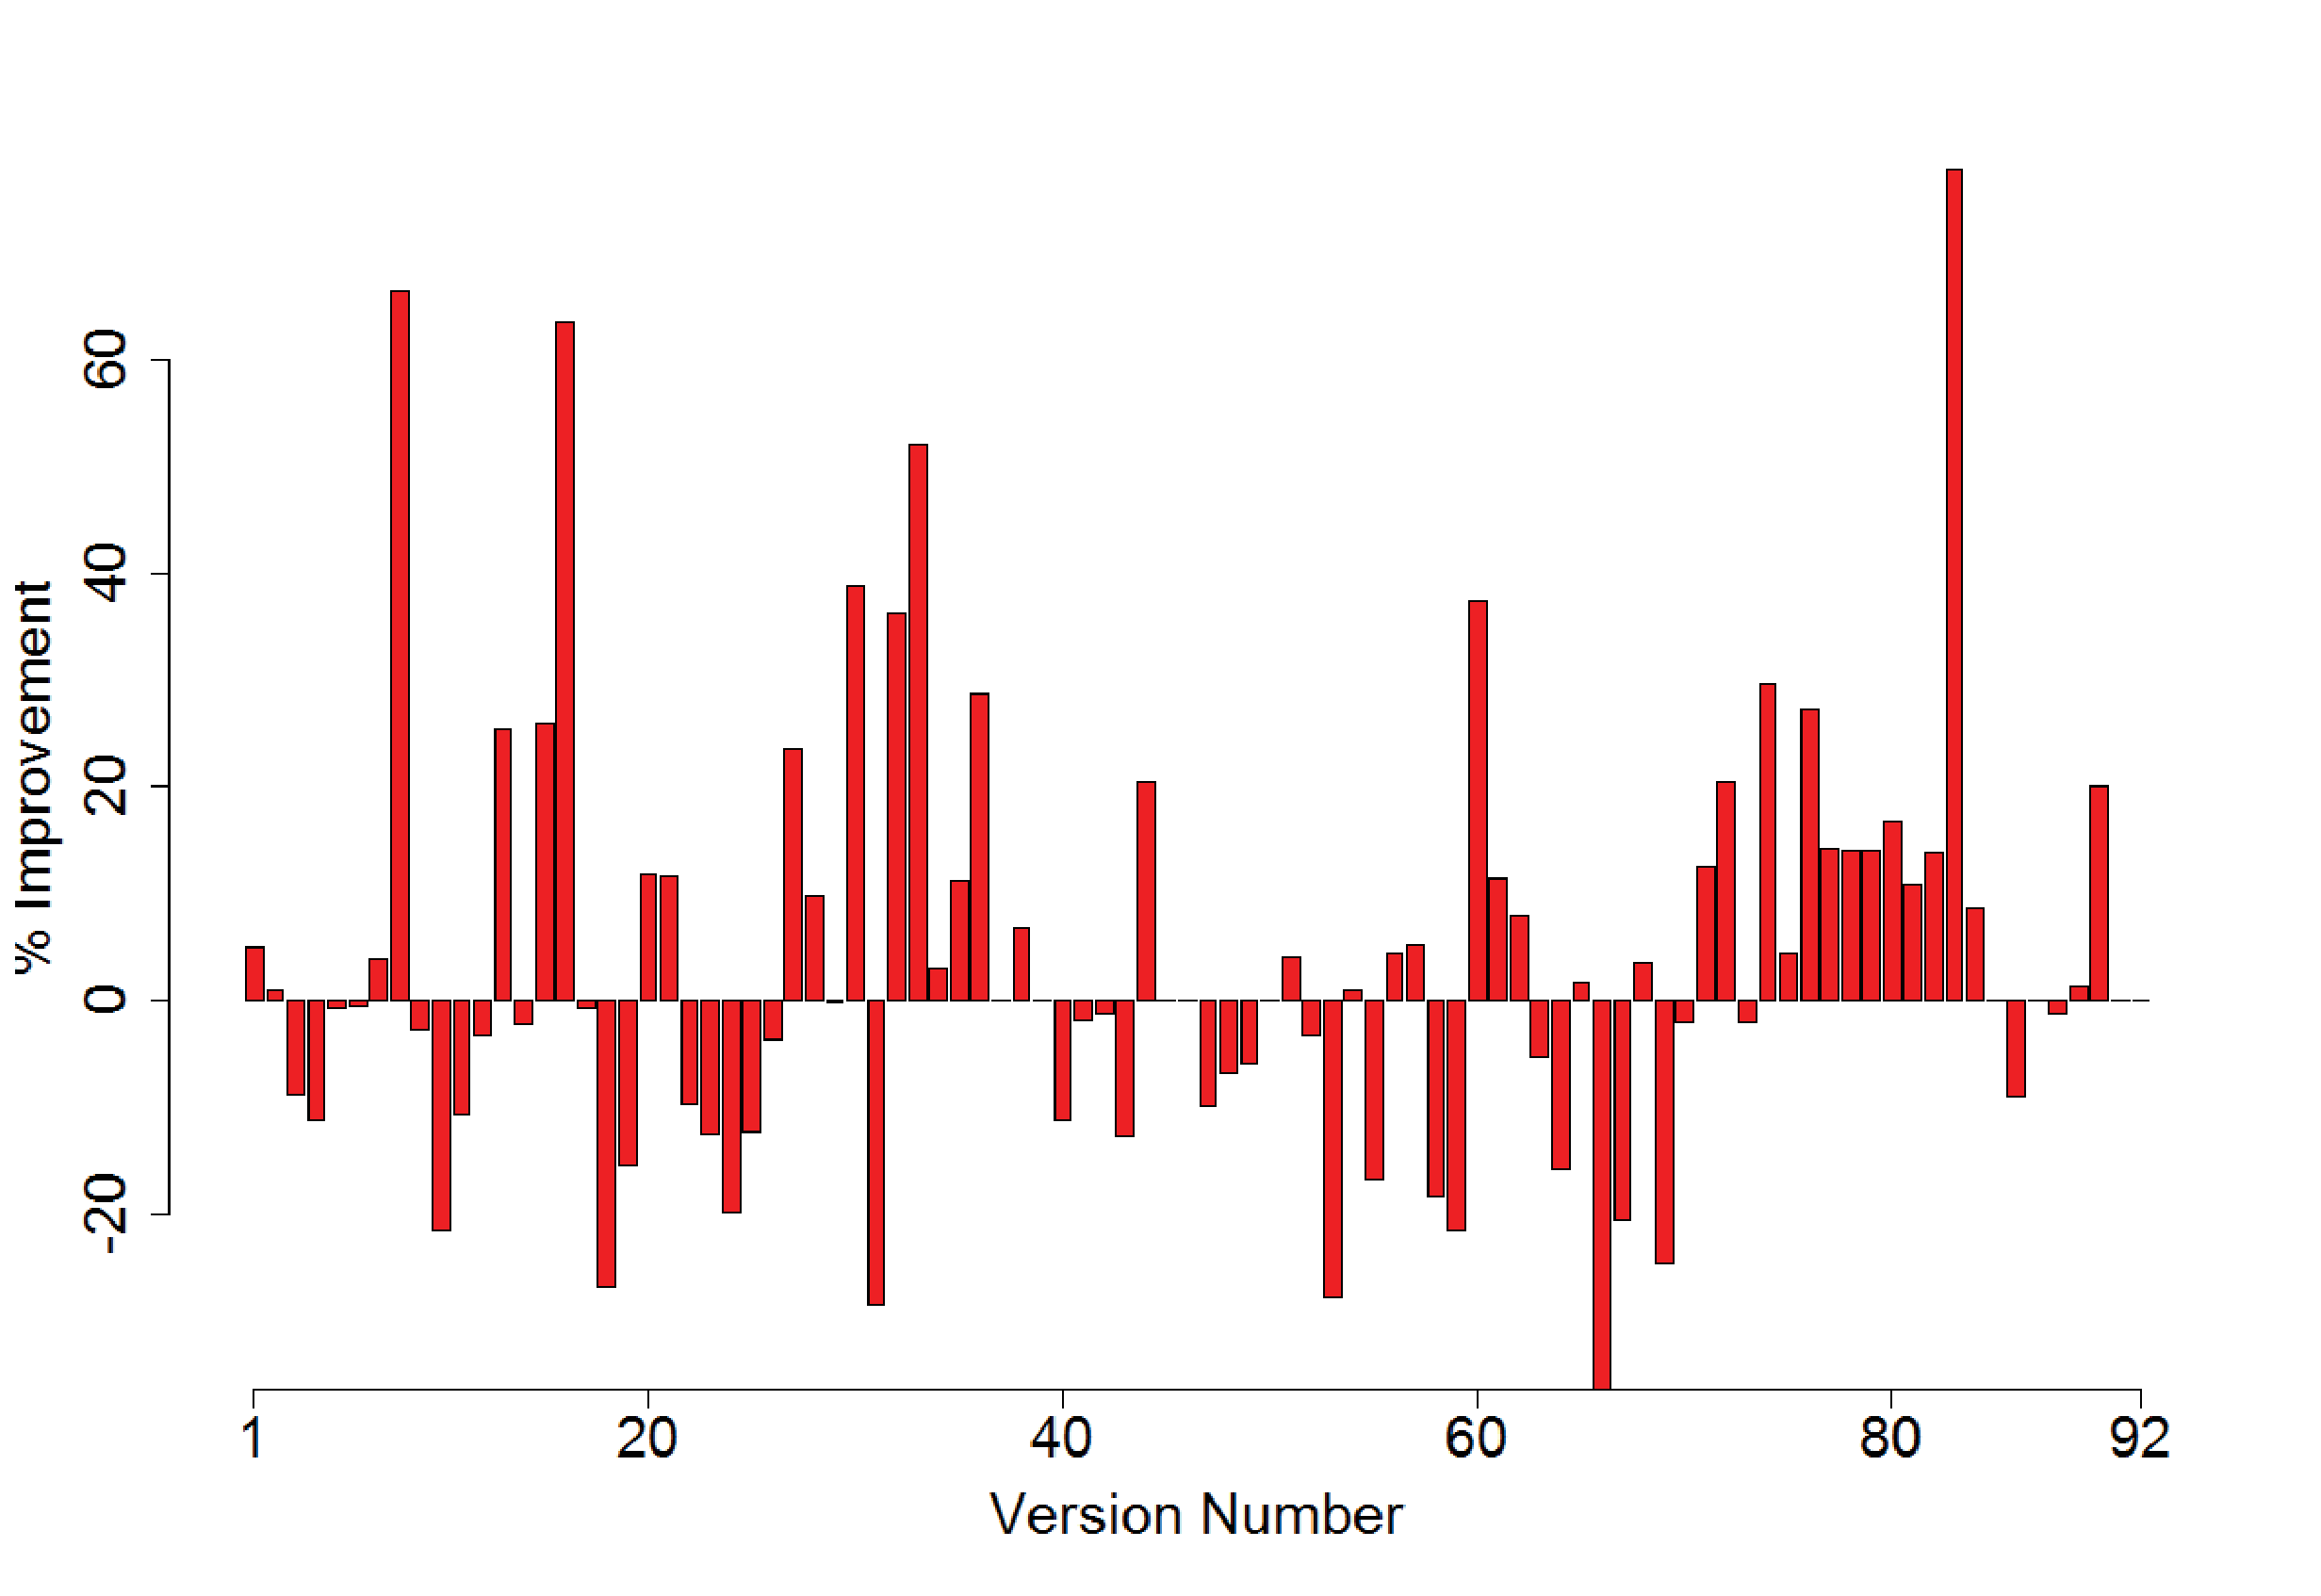
\includegraphics[width=0.6\textwidth]{QRM_allFail.eps}
\caption{Relative performance of NUMFL-GPS-QRM with and without data from passing runs, on individual single-fault program versions.}
\label{QRM_allFail}
\end{figure*}

From Table \ref{table3} and Figure \ref{QRM_allFail}, we can see that NUMFL works fairly well for most subject programs when used with data from only failing runs, although its performance is generally better with data from both passing and failing runs.  Note that with many numerical programs the tolerance for output errors is very small (between 1.0E-5 and 1.0E-12).  For such programs, the output errors from passing runs are clustered around 0, while output errors from failing runs are larger and more varied.  Consequently, the data from failing runs carries more information about the dose-response function than does the data from the passing runs.  Hence, using only data from failing runs to estimate the DRF does not necessarily result in severe bias.

\subsection{Application of NUMFL-GPS to Programs with Multiple Faults}
The empirical results presented in Section \ref{VD} indicate that NUMFL-GPS performs better than the baseline techniques on the subject program versions containing a single fault.  This section reports on the application of NUMFL-GPS to subject program versions with multiple faults.  For this sub-study, we selected five of the larger subject programs (shown in Table \ref{table4}) and generated 5 faulty versions of each for a total of 25 faulty versions.  To create each faulty version, we randomly injected two simulated faults. (Injecting a larger number of faults in our programs tended to make them fail badly on all inputs).  Table \ref{table4} shows the average cost, over the faulty versions of each subject program, of localizing the first fault to be found, for NUMFL-GPS-QRM and each of the baseline techniques.  The table shows that NUMFL-GPS-QRM outperformed the other baseline techniques on average, although SOBER and Ochiai each performed better on one of the subject programs.
\begin{table*}[htbp!]
\fontsize{8pt}{9pt}\selectfont
\centering
\caption{AVERAGE FAULT LOCALIZATION COSTS OF NUMFL-GPS-QRM AND BASELINE METRICS ON SINGLE-FAULT PROGRAM VERSIONS}
\label{table4}
      \begin{tabular}{|l|c|c|c|c|c|c|}
      \hline
\multirow{2}{*}{{\bf Subject Program}}	&	\multicolumn{6}{|c|}{{\bf Technique}}	\\	\cline{2-7}
&{NUMFL-GPS-QRM}	&Ochiai&	Dstar&	ESP(SIV) &	ESP(SCP)	&SOBER \\\hline
Apache\_EigenDecompose	&	10.3\%	&	20\%	&	19.4\%	&	28.3\%	&	25.8\%	&	6.3\%	\\	\hline
Apache\_DScompiler	&	4.5\%	&	31.5\%	&	23.2\%	&	19.9\%	&	10.4\%	&	9\%	\\	\hline
Apache\_Rotation3D	&	7\%	&	3.6\%	&	33.6\%	&	17.5\%	&	17.9\%	&	25.8\%	\\	\hline
Ojaljo\_SchurDecompose	&	5.4\%	&	22.7\%	&	27.1\%	&	8.4\%	&	9.6\%	&	27.1\%	\\	\hline
Jama\_MatrixDecompose	&	14.1\%	&	26.3\%	&	16.5\%	&	26.3\%	&	26.2\%	&	15.5\%	\\	\hline
Average Cost	&	8.3\%	&	20.8\%	&	24\%	&	20.1\%	&	18\%	&	16.7\%	\\	\hline
\end{tabular}
\end{table*}

Figure \ref{QRM_VS_Base_MultipleFault} graphically contrasts the performance of NUMFL-GPS-QRM on the individual two-fault program versions with that of the baseline metrics.  It is evident that SOBER's performance is the second best after NUMFL-GPS-QRM.  Over all 25 faulty subject-program versions, NUMFL-GPS-QRM performed better than SOBER on 15 versions but performed worse on 10 versions.  There were 8 versions for which NUMFL-GPS-QRM performed at least 10\% better than SOBER but only one version for which SOBER performed at least 10\% better than NUMFL-GPS-QRM.  Both Ochiai and ESP-SCP performed better than NUMFL-GPS-QRM on 8 versions but performed worse on 17 versions.  NUMFL-GPS-QRM performed better than ESP-SIV on 19 versions and performed better than DStar on 21 versions.
\begin{figure*}[!thpb]
\centering
\includegraphics[width=\textwidth]{QRM_VS_Base_MultipleFault.eps}
\caption{Performance of GPS-QRM relative to baseline metrics on individual two-fault program versions .}
\label{QRM_VS_Base_MultipleFault}
\end{figure*}

\subsection{Comparison of NUMFL-GPS and NUMFL-CBPS}
In this section, we report the results of empirically comparing the performance of NUMFL-GPS-QRM with that of NUMFL-CBPS-QRM.  We applied the two techniques to the subject program versions with single faults as well as to the versions with two faults.  The average fault localization costs on the single fault versions is shown in Table \ref{table5}.  There were 13 versions for which NUMFL-GPS-QRM performed better than NUMFL-CBPS-QRM. There were only 3 versions for which NUMFL-CBPS-QRM performed better than NUMFL-GPS-QRM. Figure \ref{CBPS_VS_GPS} graphically contrasts the performance of the two methods on the single fault versions.  NUMFL-GPS-QRM performed better on 61 versions, while NUMFL-CBPS-QRM performed better on 31 versions.  NUMFL-GPS-QRM performed at least 20\% better than NUMFL-CBPS-QRM on 15 versions, whereas NUMFL-CBPS-QRM performed at least 20\% better than NUMFL-GPS-QRM on just 4 versions.

\begin{table*}[htbp!]
\caption{AVERAGE FAULT LOCALIZATION COSTS OF NUMFL-GPS-QRM AND NUMFL-CBPS-QRM ON SINGLE-FAULT PROGRAM VERSIONS }
\label{table5}
\centering
      \begin{tabular}{|l|c|c|}
      \hline
\multirow{2}{*}{{\bf Subject Program}}	&	\multicolumn{2}{|c|}{{\bf NUMFL}}	\\	\cline{2-3}
&  GPS-QRM	&CBPS-QRM \\ \hline
Apache\_EigenDecompose	&	12.3\%	&	8.8\%	\\	\hline
Apache\_DScompiler	&	11\%	&	12\%	\\	\hline
Apache\_BigMatrix	&	11.4\%	&	9.9\%	\\	\hline
Apache\_Rotation3D	&	8\%	&	18.9\%	\\	\hline
Ojaljo\_SchurDecompose	&	11.4\%	&	14\%	\\	\hline
Jama\_MatrixDecompose	&	14.2\%	&	23\%	\\	\hline
SciMark\_LU	&	15.3\%	&	27.8\%	\\	\hline
SciMart\_FFT	&	9.5\%	&	19.8\%	\\	\hline
Apache\_SymmLQ	&	2.6\%	&	4.4\%	\\	\hline
Apache\_SplineInterpolator	&	31.7\%	&	35\%	\\	\hline
Apche\_SimpleRegress	&	4.3\%	&	17\%	\\	\hline
Apache\_SchurTransformer	&	3.3\%	&	14.9\%	\\	\hline
Apache\_MillerUpdatRegress	&	7.5\%	&	9.9\%	\\	\hline
Apache\_HarmonicFitter	&	27.3\%	&	32\%	\\	\hline
Apache\_FastSine	&	1.5\%	&	13\%	\\	\hline
Apache\_FastCosine	&	1.3\%	&	1.2\%	\\	\hline
Average Cost	&	10.8\%	&	16.4\%	\\	\hline
\end{tabular}
\end{table*}

Table \ref{table6} shows the average cost, over the faulty versions of each subject program into which two faults were injected, of localizing the first fault to be found, for both NUMFL-GPS-QRM and NUMFL-CBPS-QRM.  NUMFL-GPS-QRM performed better than NUMFL-CBPS-QRM on the two-fault versions of 4 subject programs. NUMFL-GPS-QRM performed worse than NUMFL-CBPS-QRM on the versions of 1 subject program.  Figure \ref{CBPS_VS_GPS_MultipleFault} graphically contrasts the performance of the two methods on the individual two-fault versions.  NUMFL-GPS-QRM performed better than NUMFL-CBPS-QRM on 13 versions and NUMFL-GPS-QRM performed worse on 12 versions.  NUMFL-GPS-QRM performed at least 10\% better than NUMFL-CBPS-QRM on 7 versions, whereas NUMFL-CBPS-QRM performed at least 10\% better than NUMFL-GPS-QRM on just 1 version.

In summary, NUMFL-GPS-QRM performed better than NUMFL-CBPS-QRM on both single-fault and two-fault programs.  The generalized propensity score model $\pmb{\theta}=\pmb{X}'\pmb{\beta}$ achieved better covariate balance than the multinomial logistic regression model used with CBPS.  This may be due to the composition of the data collected from our subject program versions.  The performance of NUMFL-CBPS was poorest with versions that had no more than about 150 failing executions.  However, although NUMFL-CBPS performed worse than NUMFL-GPS in our study, the former's average fault localization cost was still lower than those of the baseline techniques.
\begin{table*}[htbp!]
\caption{AVERAGE FAULT LOCALIZATION COSTS OF NUMFL-GPS-QRM AND NUMFL-CBPS-QRM ON MULTIPLE-FAULT PROGRAM VERSIONS}
\label{table6}
\centering
      \begin{tabular}{|l|c|c|}
      \hline
\multirow{2}{*}{{\bf Subject Program}}	&	\multicolumn{2}{|c|}{{\bf NUMFL}}	\\	\cline{2-3}
&  GPS-QRM	&CBPS-QRM \\ \hline
Apache\_EigenDecompose	&	10.3\%	&	11.1\%	\\	\hline
Apache\_DScompiler	&	4.5\%	&	5.9\%	\\	\hline
Apache\_Rotation3D	&	7.0\%	&	3.0\%	\\	\hline
Ojaljo\_SchurDecompose	&	5.4\%	&	19.8\%	\\	\hline
Jama\_MatrixDecompose	&	14.1\%	&	23.4\%	\\	\hline
{\bf Average Cost} & 8.26\% &12.64\%\\ \hline
\end{tabular}
\end{table*}

\begin{figure*}[!thpb]
\centering
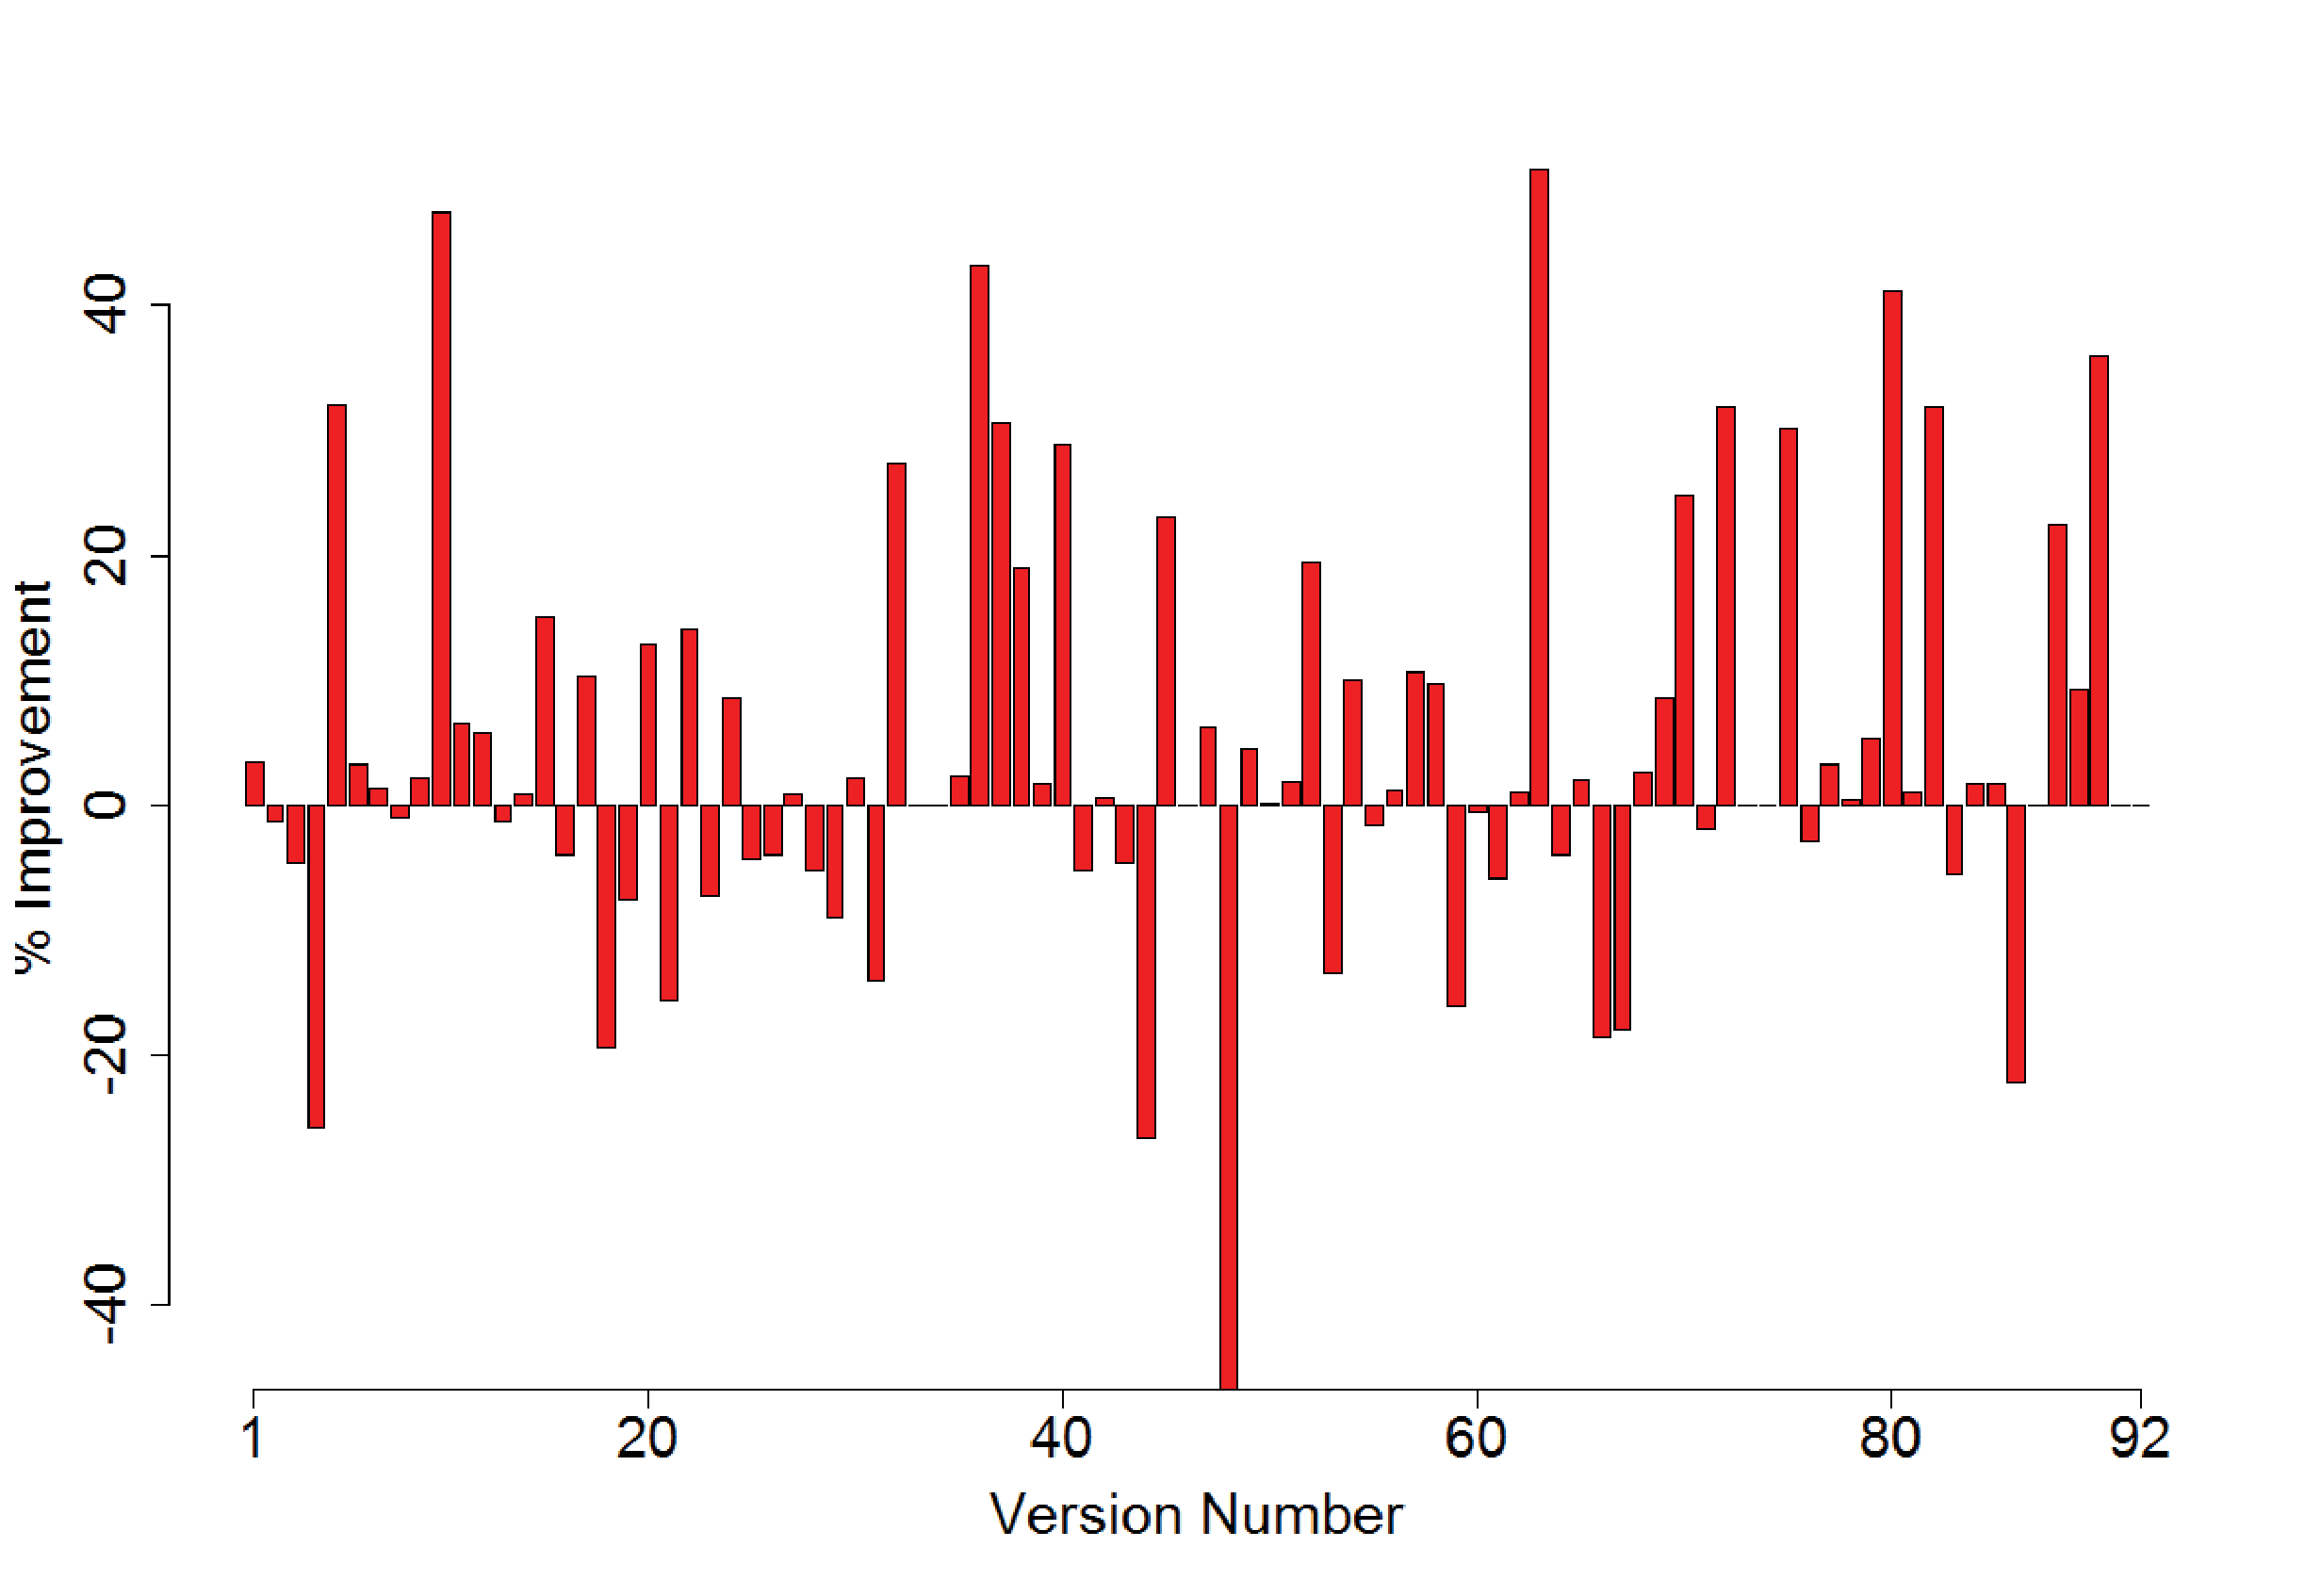
\includegraphics[width=\textwidth]{CBPS_VS_GPS.eps}
\caption{. Relative performance of NUMFL-GPS-QRM and NUMFL-CBPS-QRM on individual single-fault program versions .}
\label{CBPS_VS_GPS}
\end{figure*}

\begin{figure*}[!thpb]
\centering
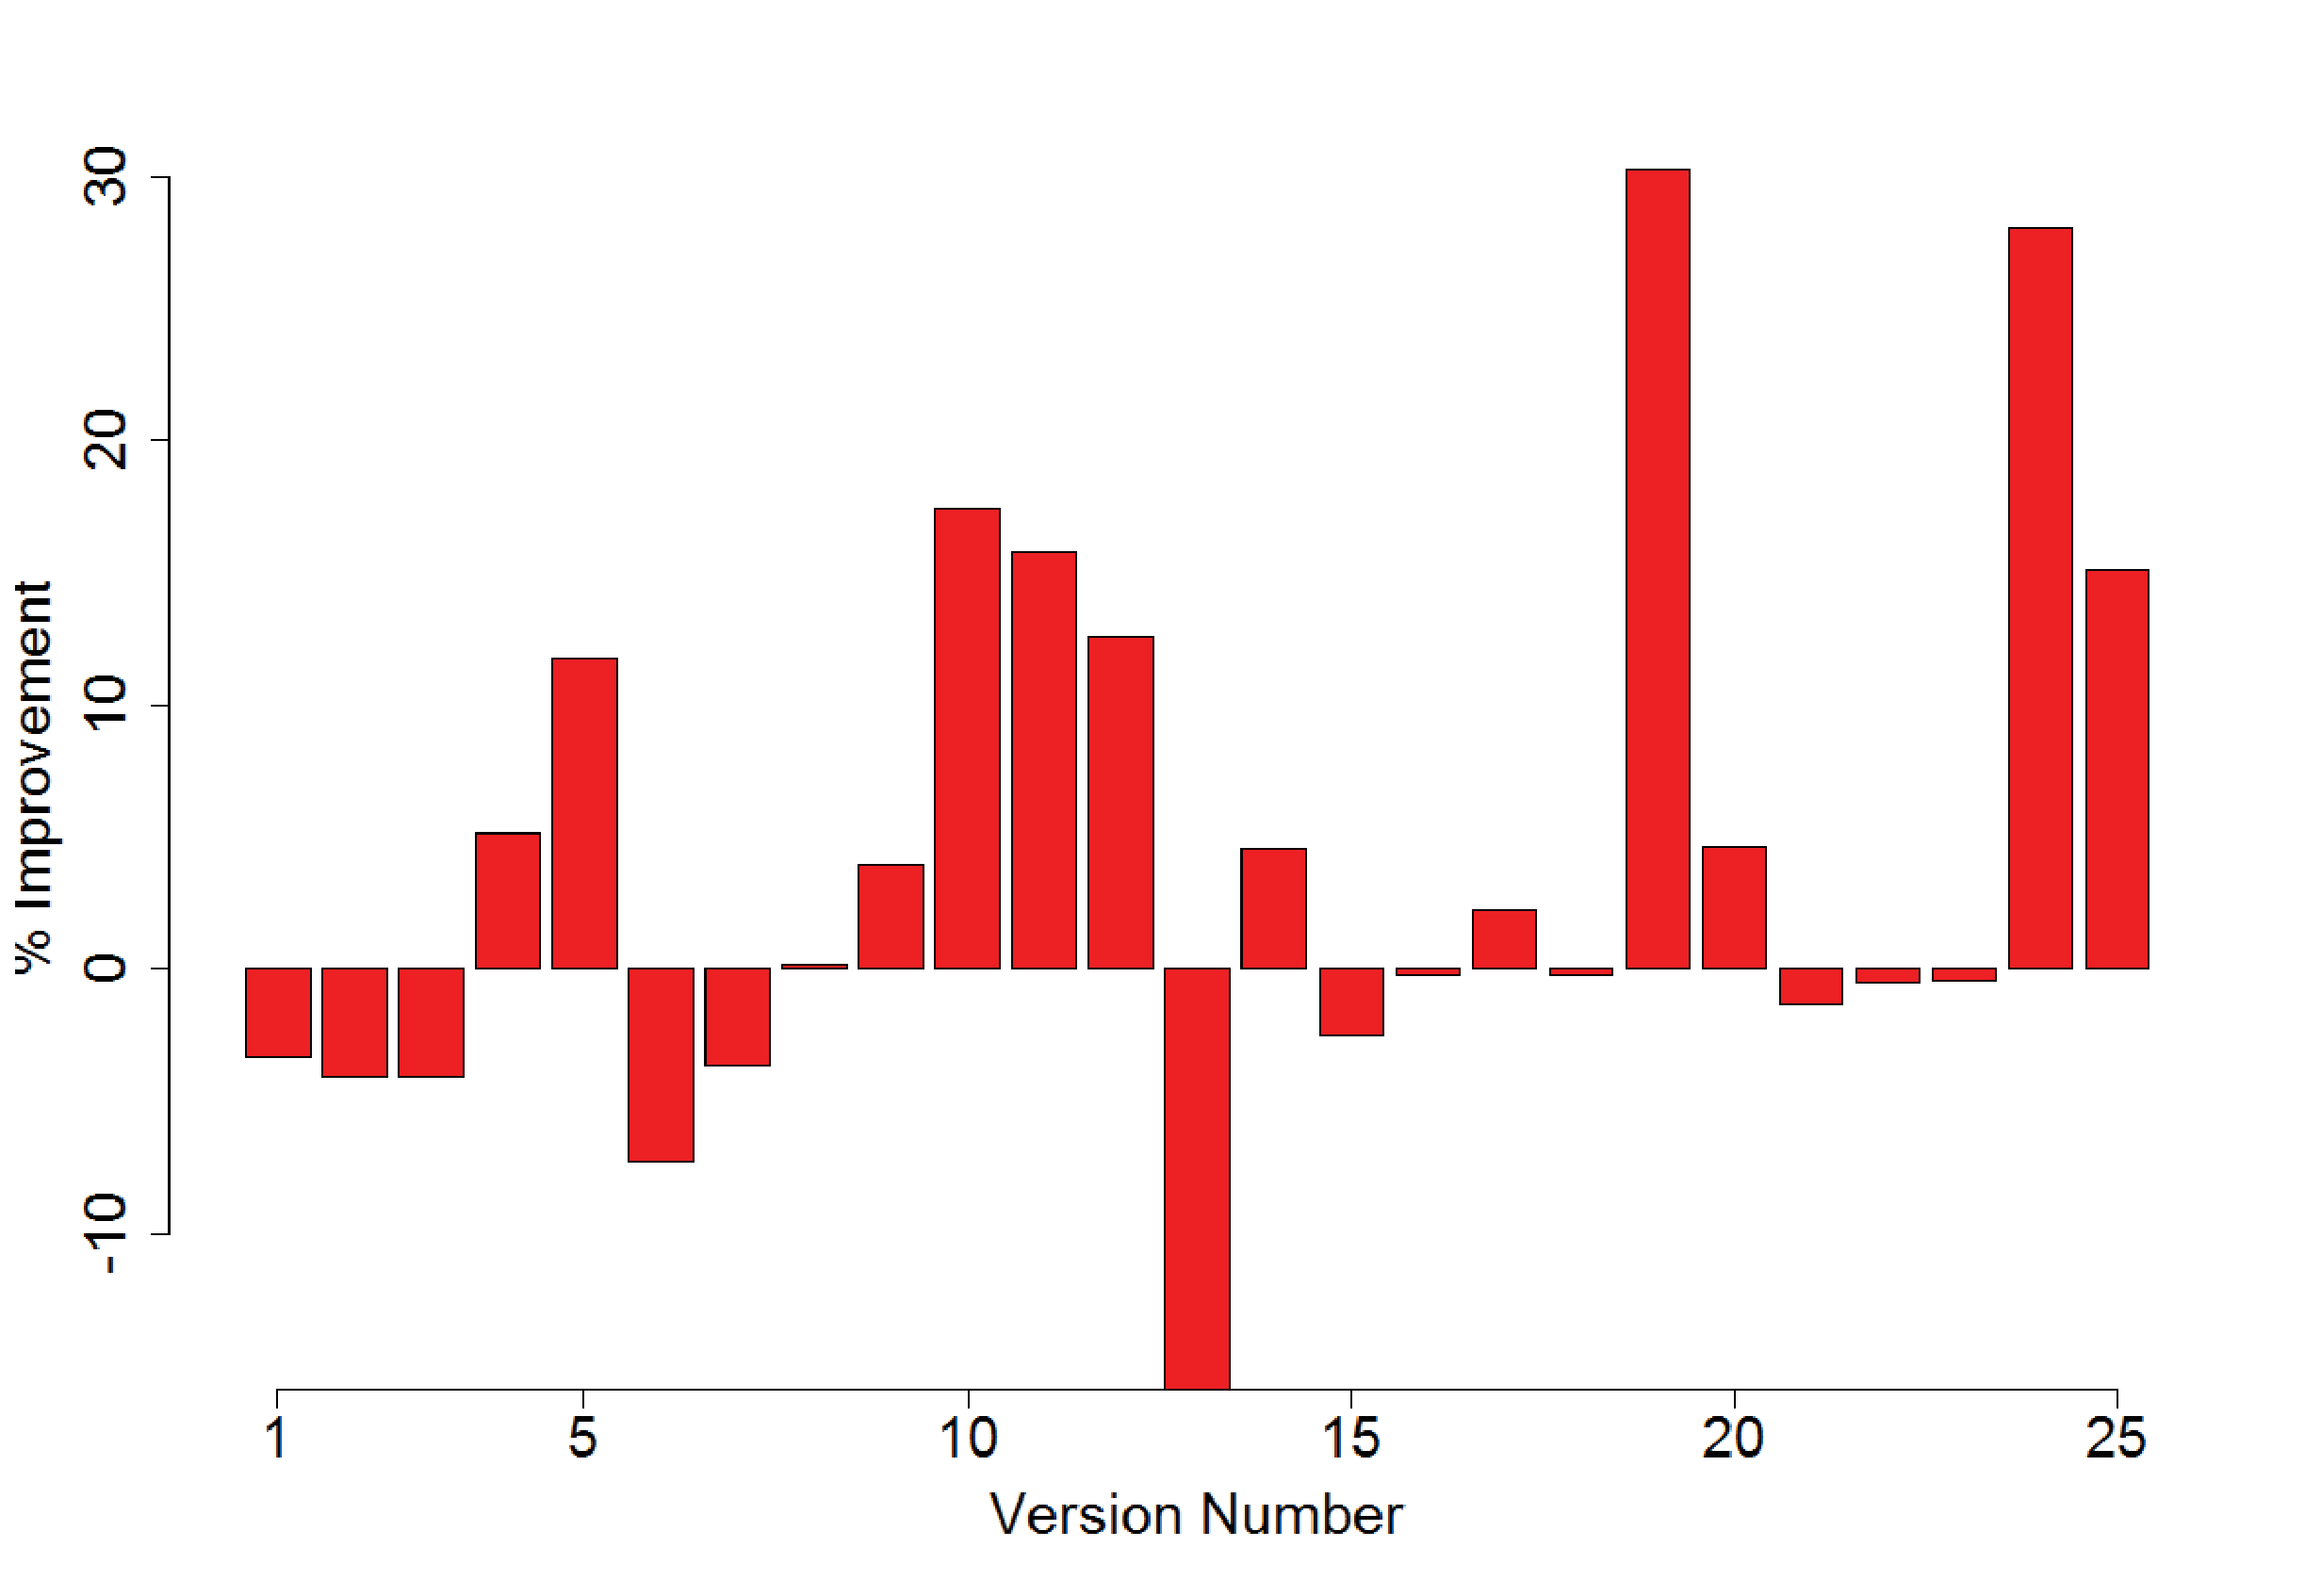
\includegraphics[width=\textwidth]{CBPS_VS_GPS_MultipleFault.eps}
\caption{Relative performance of NUMFL-GPS-QRM and NUMFL-CBPS-QRM on individual two-fault program versions .}
\label{CBPS_VS_GPS_MultipleFault}
\end{figure*}

\subsection{Limitations}
NUMFL and its evaluation are subject to several limitations.  First, NUMFL employs regression models for two purposes: estimating generalized propensity scores and estimating the causal effect of the treatment on the outcome.  We used Gaussian (Normal) linear models for both purposes in NUMFL-GPS, because they are supported by fast and robust software, and they performed well in our empirical study. In NUMFL-CBPS, we use multinomial logistic regression propensity score models.  However, other model choices may be more appropriate for applying NUMFL to different numerical software.  Determining that would require preliminary analysis of the data.  A related issue is that sufficient data must be available to adequately fit each model.  We have found that the number of failing tests should at least 100 to fit adequate regression models.  This is not a serious problem, since faults in numerical programs are usually not guarded by many branch conditions that are likely to cause ``coincidental correctness."  A limitation of our empirical study is that the seeded faults were of three basic types.  In future work, we intend to evaluate NUMFL on subject programs with more varied faults.  Finally, validity of NUMFL (with QRM) depends on Assumptions 1 and 3 in section \ref{twoversion}.  These assumptions do not always hold in practice.  For example, if the effect of a numerical fault does not propagate to the output (coincidental correctness), then Assumption 3 will be violated.

\section{RELATED WORK}\label{relatedwork}
The seminal SFL research of Jones et al. \cite{Jones2002}, which is coverage based, and of Liblit et al. \cite{Liblit2005}, which is predicate based, has inspired much subsequent research.  The use of causal inference methodology in SFL is due to Baah et al. \cite{Baah2010}.  They showed that estimating the AFCE of covering a statement $s$ using a linear regression model that adjusts for coverage of the direct control dependence predecessor of $s$ is effective for reducing confounding bias that often distorts fault localization scores.  Later, Baah et al. \cite{Baah2011} extended this work by using covariate matching to control confounding bias involving both control and data dependence predecessors.  More recently, Gore et al. \cite{Gore2012} extended Baah's initial approach by providing a model that reduces what they called ``failure flow confounding bias," which involves predicate outcomes.  Recently, Shu et al. \cite{Shu2013} proposed a method-level causal inference model to localize faulty methods in large programs. The aforementioned techniques, unlike NUMFL, do not use values of program variables in fault localization.

State-altering techniques, such as {\it cause-transitions} \cite{Cleve2005} and {\it value replacement} \cite{Jeffrey2008} are among the few fault localization techniques based on values of variables.  Cause-transitions employs {\it delta debugging} \cite{Zeller2002} to isolate the cause of a program failure. Value replacement localizes faults by switching program states and re-running the program. Unlike SFL techniques, these techniques actually alter program states, and they require an oracle to determine if alterations cause program failures. On the other hand, they are non-statistical and do not require a sample of both passing and failing executions. The {\it Daikon} system identifies possible invariant conditions in a program based on a sample of executions \cite{Ernst2007}. The {\it DIDUCE} system uses Daikon to report violations of dynamic invariants, which may indicate failures \cite{Hangal2002}. However, these techniques do not address confounding bias.


Some recent studies have developed techniques to analyze instability in floating-point computations. {\it CADNA} \cite{Scott2007} is a library to estimate round-off errors with Monte-Carlo Arithmetic. Tang et al. \cite{Tang2010} proposed a technique to automatically detect such errors by systematically altering the underlying numerical calculation. Lam et al. \cite{Lam2013} proposed to use the detection of significant digit cancellation events to test the precision of numerical programs.  Later, Zhang et al. \cite{Bao2013} extended Lam's work by monitoring the propagation of cancelled bits.  These studies focused on detecting accumulated round-off errors due to finite-precision computation, but they do not address the problem of localizing faults in numerical expressions generally.


Other researchers have proposed alternatives to Imai and van Dyk's approach to defining and using the generalized propensity score.  Hirano and Imbens estimate the causal effect of a continuous treatment variable by fitting one regression model with the GPS as a predictor \cite{Hirano2004}. This method requires discretizing the treatment variable when calculating the propensity score.  Zhao and Imai extend Hirano and Imbens's work by using a smooth coefficient model (SCM) in the regression, so the model can estimate the dose-response function of the treatment variable instead of average causal effect \cite{Zhao2013}.  In preliminary work (with different subject programs), we found that these GPS methods did not perform as well as Imai and Van Dyk's approach, which is used in this paper.


\section{CONCLUSION}\label{conclusion}
In this chapter, we have presented and evaluated a value-based causal model, denoted NUMFL, for localizing faults in numerical software. NUMFL employs generalized propensity scores and covariate balancing propensity scores to control confounding bias involving floating-point program variables that carry erroneous values to correct statements.  NUMFL uses a quadratic regression model (QRM) to estimate the average failure-causing effect of a numerical expression.  We reported the results of an empirical comparison of NUMFL to several competing techniques on both single-fault subject programs and multiple-fault subject programs.  NUMFL performed notably better than the other techniques. We also found that NUMFL-GPS works well with data from failing {\it runs alone}.  Finally, we compared the performance two versions of NUMFL, denoted NUMFL-GPS and NUMFL-CBPS, based on the two aforementioned types of propensity scores. We found that the NUMFL-GPS performed better than NUMFL-CBPS for both single-fault programs and two-fault programs.   In the future work, will seek to extend our empirical results to a broader range of subject programs with more varied fault types.  We intend eventually to evaluate NUMFL in a user study, but given the difficulty of conducting an unbiased one, we think it is desirable to refine NUMFL as much as possible beforehand.  Finally, we will also explore the integration of NUMFL with coverage or predicate based causal SFL techniques. 
\chapter{Causal Inference Based Fault Localization for Numerical Software with Bayesian Additive Regression Trees}\label{chap:BART}


\section{Introduction}\label{BARTintro}
\vspace{-2pt}
Average failure causing effect estimation is challenging when the outcome $Y$ is not linearly related to the treatment $T$ and confounders $X$. Previous work like NUMFL estimates AFCE with non linear parametric regression model \cite{bai2015numfl}, which depends on some pre-assumptions of the relationship between $T$ and $Y$, given the confounding variable $X$ is well controlled.  If any assumption does not hold, then the AFCE estimation can be biased. Bayesian Additive Regression Trees(BART), a new causal effect estimation method has been proposed in the past few years. It is requires less guess-work in model fitting and handles the large number of predictors.
  
In this chapter, we proposal a new statistical fault localization method based on BART model and evaluate it on numerical programs with single or multiple faults. The motivation for using BART in statistical fault localization is:
\vspace{-0.2cm}
\begin{itemize}
\item BART can flexibly fit non-linear response surfaces even with a large number of predictors
\item BART does not require the researcher to specify the functional form of the relationship between treatment and outcome. The user only need to input the treatment, confounding variable and the outcome, but not need to provide how these variables are parametrically related. Also, comparing to methods such as propensity score matching and subclassification, BART produces coherent posterior predictions.
\item The casual inference techniques has been proved to be effective in both coverage based fault localization and value based fault localization. The treatment effect estimated with BART appear to be substantially more accurate than linear regression, and propensity score matching with regression adjustment when the treatment variable is binary. It has potential in estimating failure-causing effect for continuous treatment \cite{hill2012bayesian, hill2013assessing}.
\item BART algorithm software is freely available and easy to use \cite{BARTMachine}.
\end{itemize}

The rest of the chapter is organized as follows: we present the background of single regression tree and BART model in Section \ref{BARTbg}; Using BART model to estimate failure-causing effect is described in detail in Section \ref{BARTafce};  we report on its empirical evaluation in Section \ref{BARTevaluation}; related work is surveyed in Section \ref{BARTrelatedwork}; and Section \ref{BARTconclusion} concludes the chapter.

\section{BART Model Algorithm}\label{BARTbg}%what is BART and why BART
The BART model algorithm consists of three parts: a sum of regression trees model, a regularization prior and a fitting algorithm Marcov Chain Mote Carlo (MCMC)
\subsection{A Single Regression Tree model}\label{IIIA}
Regression tree is one type of decision tree that predicts the value of a target variable based on several input variables. Regression tree handles the situation when the target variable is continuous. Figure \ref{singlergt} shows a single regression tree model. All the interior nodes of a regression tree have decision rules which send the input data set to either left or right side. After the input data set go through the interior nodes and reach the bottom of the tree, the data set is divided into several disjoint subgroup. Each group of data is represent by a leaf node.

\begin{figure*}[!thpb]
\centering
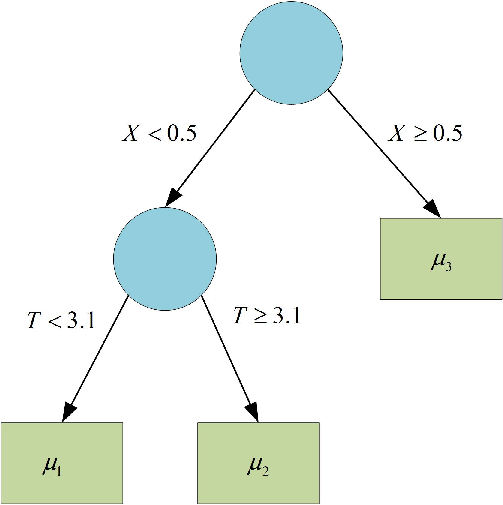
\includegraphics[width=0.5\textwidth]{chapter4_SingleRGT.pdf}
\caption{Single Regression Tree Structure}
\label{singlergt}
\end{figure*}

A single regression tree model is denoted as:
\begin{equation*}
Y=g(\pmb{Z}; R, M)+\epsilon
\end{equation*}
Here $\varepsilon  \sim N(0,{\sigma ^2})$ is a normal distributed error .$\pmb{Z}=[T,\pmb{X}]$ denotes all the variables related to the outcome $Y$, so $Z$ includes both treatment variable $T$ and confounding variables $\pmb{X}$. $R$ denotes a binary regression tree consisting a set of interior node decision rules and a set of terminal nodes, and let $M=
\begin{Bmatrix}
 \mu _1, \mu _2, . . ., \mu _b
\end{Bmatrix}$
denotes a set of parameter value associated with each of the $b$ terminal nodes of $R$. Each terminal node represent a regression model of outcome $Y$ on all the variables $Z$.

A regression tree model is often used in approximating unknown functions. For example, if the causal effect of treatment $T$ on outcome $Y$ is decided by an unknown function $Y=f(T,\pmb{X})$, then we can approximate the function $f(T,\pmb{X})$ by fitting a single regression tree model g(\pmb{Z}; R, M) on sample data set. The regression tree model divides the value space of $[T,\pmb{X}]$ in to several subgroups with its tree structure and fit a regression model for each subgroup. When making inference of $Y$ given a specific unit of treatment and confounding variables values $[T=t,\pmb{X}=\pmb{x}]$, the regression will first find out which subgroup the unit belongs to and then infer outcome $Y$ with the corresponding linear regression. Regression tree model has two advantages: (1) making prediction is fast. (2) it can handle non-linear function approximation.


\subsection{A sum of regression trees model}
BART model is a sum of trees model. With the definition of a single tree model, the sum of trees model can be expressed as:
\begin{equation*}
Y = g(\pmb{Z};{R_1},{M_1}) + g(\pmb{Z};{R_1},{M_1}) +  \cdots  + g(\pmb{Z};{R_m},{M_m}) + \varepsilon
\end{equation*}
where each $(R_i,M_i)$ denotes a single sub-tree model and $\varepsilon  \sim N(0,{\sigma ^2})$.  $m$ denotes the number of trees in BART model. We have
 \begin{equation*}
 Y =f(\pmb{Z})=f(T,\pmb{X})= \left( {\sum\limits_{j = 1}^m {g(T,\pmb{X};{R_j},{M_j})} } \right) + \varepsilon
 \end{equation*}

Comparing to single regression tree model, BART model has two advantages. First BART is more naturally handle the interaction effects . In the sum of trees model, each tree explains part of the overall fit, so there are many different choices of $(R_1,M_1) \cdots (R_m,M_m)$ can lead to an identical function$ \sum\limits_{j = 1}^m {g(T,\pmb{X};{R_j},{M_j})} $. Second, BART can scale to large datasets using a parallel MCMC sampler \cite{pratola2014parallel, pratola2015bayesian}. Thus, fitting BART model does not has much more computation cost than fitting a large single tree model.

\subsection{A regularization prior}
Fitting the BART model requires a prior of all the parameters of the sum of trees model.  The prior regularize the fit by keeping the individual tree's effect from being unduly influential. Without such a prior, large  tee components would dominate the sum of trees structure. The regularization prior can also help BART avoid overfitting. To simplify the prior specification, the trees in BART model $(R_1, M_1), (R_2,M_2), \ldots, (R_m, M_m) $ are considered to be independent of each other and of $\sigma$. Also, the terminal node parameters $ \mu _{1j}, \mu _{2j}, . . ., \mu _{bj} $ of every tree $R_j$ are independent. So we have:

\begin{equation*}
 \begin{array}{l}
P(({R_1},{M_1}),({R_2},{M_2}) \ldots ,({R_m},{M_m}),\sigma ) = \left[ {\prod\limits_j {P({R_j},{M_j})} } \right]p(\sigma )\\
\quad \quad \quad \quad \quad \quad \quad \quad \quad \quad \quad \quad \quad \quad \; = \left[ {\prod\limits_j {P({M_j}|{R_j})P({R_j})} } \right]p(\sigma )
\end{array}
 \end{equation*}
and
\begin{equation*}
P({M_j}|{R_j}) = \left[ {\prod\limits_i {P({\mu _{ij}}|{R_j})} } \right]
 \end{equation*}
Here ${\mu _{ij}} \in {M_j}$ denotes the $ith$ terminal node of the $jth$ regression tree From the above equations, we can see the independence simplify the prior specification problem to the specification of prior for just ${P({\mu _{ij}}|{R_j})}$, $P({R_j})$ and $P(\sigma)$. In \cite{chipman2010bart}, the specification of prior forms on $P(\sigma)$ is defined as the inverse chi-square distribution. The prior on ${P({\mu _{ij}}|{R_j})}$ is defined as conjugate normal distribution. The prior on $P(R_j)$ is complicated which contains 3 aspects:
\begin{enumerate}
\item the probability that a nonterminal node at depth $d$ is given by
\begin{equation*}
\alpha {(1 + d)^{ - \beta }},\quad \alpha  \in (0,1),\beta  \in [0,\infty )
 \end{equation*}
\item the prior probability that a variable is selected as the splitting variable at an interior node is $1/k$ and $k$ is the total number of variables including both treatment and confounders.
\item the prior probability that a splitting variable split at value $x$ is $1/N$ and $N$ is the total number of observed values of the splitting variable in the sample data set.
\end{enumerate}
The detail of the prior specification for ${P({\mu _{ij}}|{R_j})}$, $P({R_j})$ and $P(\sigma)$ can be reffered to \cite{chipman2010bart}.


\subsection{Bayesian Backfitting MCMC Algorithm}
BART uses a Bayesian backfitting  MCMC algorithm to fit the model \cite{gilks2005markov}. The algorithm uses Gibbs sampler \cite{casella1992explaining}. The Gibbs sampler get $m$ successive draws of $(R_j, M_j)$ conditionally on $(R_{(j)}, M_{(j)}, \sigma)$:

\begin{equation*}
(R_j,M_j)|R_{(j)}, M_{(j)}, \sigma, Y
\end{equation*}
$j=1 \ldots m$, followed by a draw of $\sigma$ from the full conditional:

\begin{equation*}
\sigma |{R_1}, \ldots ,{R_m},{M_1}, \ldots ,{M_m},Y
\end{equation*}
Here $R_{(j)}$ represents all the trees except $R_j$, so $R_{(j)}$ will be a set of $m-1$ trees. $M_{(j)}$ is similarly defined as $R_{(j)}$.

\section{BART Model with Causal Inference}\label{BARTafce}% how to use BART

When apply BART model in estimating average causal effects, we use different algorithms for binary treatment and continuous treatment. For binary treatment, BART model primarily estimate failure-causing effects such as $E(Y(1)|\pmb{X}=\pmb{x}) - E(Y(0)|\pmb{X}=\pmb{x})=E(Y|T=1, \pmb{X}=\pmb{x})-E(Y|T=0, \pmb{X}=\pmb{x})=f(1,\pmb(x))-f(0,\pmb(x))$ . The algorithm contains the following steps:
\begin{enumerate}
\item Fit BART model using MCMC algorithm to full sample
\item Get posterior prediction for each unit by setting the treatment variable value $T=1$ and keep confounding variable value unchanged..
\item Get posterior prediction for each unit by setting the treatment variable value $T=0$ and keep confounding variable value unchanged.
\item	Calculate the difference between the posterior predictions for each unit.
\item Estimate failure-causing effect by averaging all the differences of posterior predictions.
\end{enumerate}

In step 1, the fitted BART model characterized the causal relationship between treatment $T$ and outcome $Y$ given the confounding $\pmb{X}$. We can use the fitted model to predict the outcome $Y$ under different $(T, \pmb{X})$ conditions. For a untreated unit $(T=0, \pmb{X}=\pmb{x})$,  if we set the treatment variable to 1 and then input $(T=1, \pmb{X}=\pmb{x})$ into the BART model, the output is the estimated outcome for that unit in treated condition. Similarly, we can estimate the outcome of a treated unit in untreated condition by inputing $(T=0, \pmb{X}=\pmb{x})$ into the BART model. Thus, in step2, the BART model is used to predict outcome for each unit at observed treatment condition. In step 3, the fitted BART model is used to estimate posterior predictions for each unit at counterfactual condition. Thus, the difference calculated in step 4 is the causal effect estimation for each unit. The average of these differences is failure-causing effect causal effect which is estimated in step 5.

If the treatment variable is continuous, the causal effect of treatment $T$ on outcome $Y$ is characterized by a function $r_e (T)$, which is called dose-response function in medical research. For the failure-causing effect, the dose response functions of continuous treatments are usually non-linear. For example, in Chapter 3, NUMFL use parameterized quadratic model and double linear model to approximate the dose response function within subclasses and get reasonable well result. But the parameterized model has limitations. It usually requires user to make assumptions to specify form of the dose-response function.  For example, in NUMFL, we make some assumptions ($Assumptioin 1, 2, 3$).  The  $Assumptions3$ is: executions with large absolute treatment errors have larger output errors than executions with small values of treatment errors.  Although this assumption is often holds in numeric programs, it is not always to be true. In this case,  the dose response curve of treatment $T$ on outcome $Y$ is likely to deviate from the quadratic model $Y = \zeta {T_e}^2 + \eta {T_e} + c$, which may result in a bad estimation of failure-causing effect. Comparing to parametric model used in NUMFL, BART model does not require user to make assumptions or specify the functional form of the dose response function. The sum of trees structure of BART model can approximate the non-linearity of the DRF during the training phone with MCMC.

failure-causing effect estimation is a challenge for BART model. In NUMFL, the failure-causing effect is characterized by the coefficient of the regression model.  But in BART model, the sum of trees structure does not such parameters can directly characterize the ACE. To solve this problem, we propose to estimate the treatment causal effect at each unit in the sample. The average of the treatment causal effect on all sample units is the estimated ACE. The causal effect of treatment T on outcome Y for a single unit can be estimated by increasing the treatment variable value of the unit and see how outcome changes. For example, assume a unit $i$ has treatment variable $T=t$ and confounding variables$\pmb {X}=\pmb {x}$, we can use the fitted BART model to estimate the outcome of the unit $Y=y$. Then we increase the treatment variable to $t'=t+\varepsilon$, here $\varepsilon $ is a small number. We input $T'$ and $\pmb{X}$ into the fitted BART model and get the estimated posterior $Y=y'$. Then the estimated causal effect of $T$ on $Y$ for unit $i$ is $\left| {y - y'} \right|$. The algorithm is as follows:
\begin{enumerate}
\item Fit BART model using MCMC algorithm to full sample
\item Increase the treatment variable value $t$ of each unit by $\varepsilon $. The new treatment value $t'=t+\varepsilon$ and the original confounding variables forms a new data set.
\item For each unit, calculate the difference between the posterior prediction in original data set and the posterior prediction in the new data set.
\item Estimate failure-causing effect by averaging all the differences of posterior predictions.
\end{enumerate}

In the above algorithm, the BART model fitted in first step is used to approximate a function $Y=f(T,\pmb(X))$ that specify the dose-response function of the continuous treatment $T$ and confounding variables $\pmb{X}$. Step 2 and Step 3 estimate the treatment causal effect for each sample unit. Step 4 estimate the failure-causing effect of treatment on outcome.

One problem in step 2 is how to choose the value of the small number $\varepsilon $. But treatment variables in different numerical expressions have different scale of values, it is hard to find a constant $\varepsilon$ which can make $t+\varepsilon$ be a reasonable value for all the treatments. To address this problem, we use the method illustrated by Figure\ref{bartace}.  We sort the original sample data set shown in Figure\ref{bartace} (a) in increasing order according to the value of the treatment variables.  The sorted data set is shown in Figure\ref{bartace} (b). The increased treatment variable value $t'$ in step 2 is equal to the treatment variable value $t$ of the next unit in the list and the last unit in the list will be discarded. Thus, as shown in Figure ref{bartace} (c), for a data set with $n$ observational units, we will have a new data set of $n-1$ units after increasing the treatment variable. The idea behind this method is that we want the value of treatment after increment is a reasonable value that could be observed in  other tests. Also, the value of $t'$ and the value of $t$ are likely to be in the same scale, because they are neighbor in the sorted data set.

\begin{figure*}[!thpb]
\centering
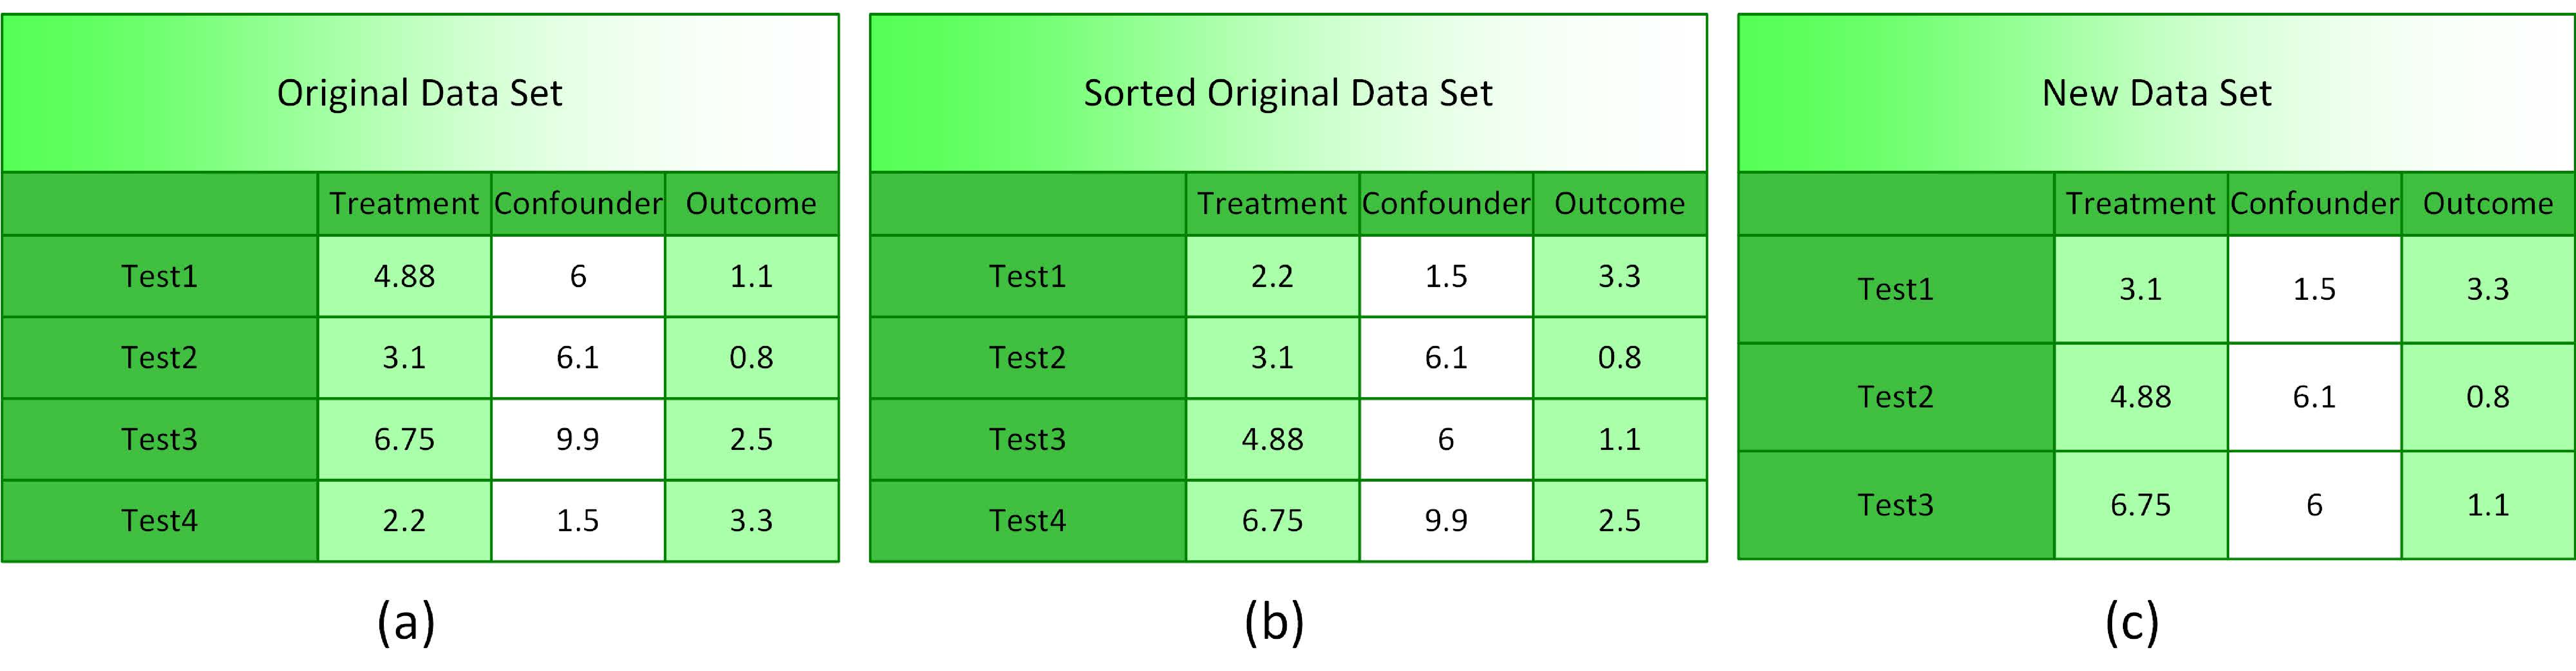
\includegraphics[width=1\textwidth]{chapter4_BART_ACE.pdf}
\caption{EXAMPLE OF TREATMENT VARIABLE INCREAMENT}
\label{bartace}
\end{figure*}

\section{EMPIRICAL EVALUATION}\label{BARTevaluation}% result

To evaluate the effectiveness of BART model, we conducted the empirical study on the same subject programs as described in chapter 3.  The tests suite is also identical to the tests suite in section \ref{numfl_evaluation}.  Overall 92 faulty subject-programs versions with single fault and 25 faulty subject-program versions with two faults. Ochiai, Dstar, SOBER, ESP-SIV are ESP-SCP used as the base line techniques to be compared with BART model. We also compare the performance of BART model with NUMFL-GPS and NUMFL-CBPS which are the proposed in chapter 3. We measured the costs of applying CBPS and the other metrics by the percentage of {\it subexpressions} that need to be examined, in decreasing order of suspiciousness scores, to find the fault, assuming the fault is recognized when it is encountered.

In the experiment, we use R package "BARTMachine" \cite{BARTMachine} to fit the BART model. We tried 10 trees and 50 trees in the sum of trees structure.  The BART model is fitted with both passing and failing tests. The number tests for each subject program is from 3000 to 8000 which shown in table \ref{subpro}. We also try to train BART model with fewer data(300 tests). the sensitivity of the BART model to the number of trees and the number of tests are discussed in section \ref{BARTsensitivity}.

\subsection{Comparative Performance of BART vs. Baselines}

Figure \ref{QRM_VS_Base} shows the results of comparisons of BART with each of the baseline metrics.  In each graph, the vertical axis represents the percentage improvement (reduction) in cost. The horizontal-axis represents different subject-program versions for which there are cost differences between the metrics, with each version represented by a vertical bar.   Bars above the zero-line represent versions for which BART performed better than the baseline metric and bars below zero represent versions for which BART performed worse.  The length of each bar represents the magnitude of the corresponding cost difference.

\textit{\textbf{ BART vs. Ochiai.}}  Over all 92 faulty subject-program versions, BART performed better than the Ochiai metric on 75 versions but BART performed worse on 17 versions.  There were 41 versions for which BART performed at least 20\% better than the Ochiai metric.  There were just 4 versions for which the latter performed better than BART.

\textit{\textbf{ BART vs. DStar.}}  BART performed better than DStar on 77 subject-program versions but BART performed worse than DStar on 15 versions.  BART performed at least 20\% better than DStar on 44 versions, whereas DStar performed at least 20\% better than BART on just 4 versions.

\textit{\textbf{ BART vs. ESP-SIV.}} BART performed better than ESP-SIV on 78 subject-program versions but BART performed worse than ESP-SIV on 14 versions.  BART performed at least 20\% better than ESP-SIV on 30 versions, whereas ESP-SIV never performed at least 20\% better than BART.

\textit{\textbf{ BART vs. ESP-SCP.}}  BART performed better than ESP-SCP on 75 subject-program versions but BART performed worse than ESP-SCP on 17 versions.  BART performed at least 20\% better than ESP-SIV on 22 versions, whereas ESP-SCP performed at least 20\% better than BART on just 2 versions.

\textit{\textbf{ BART vs. SOBER.}}  BART performed better than SOBER on 73 subject-program versions but BART performed worse than SOBER on 19 versions.  BART performed at least 20\% better than SOBER on 39 versions, whereas SOBER performed at least 20\% better than BART on just 5 versions.

\begin{sidewaysfigure}
\centering
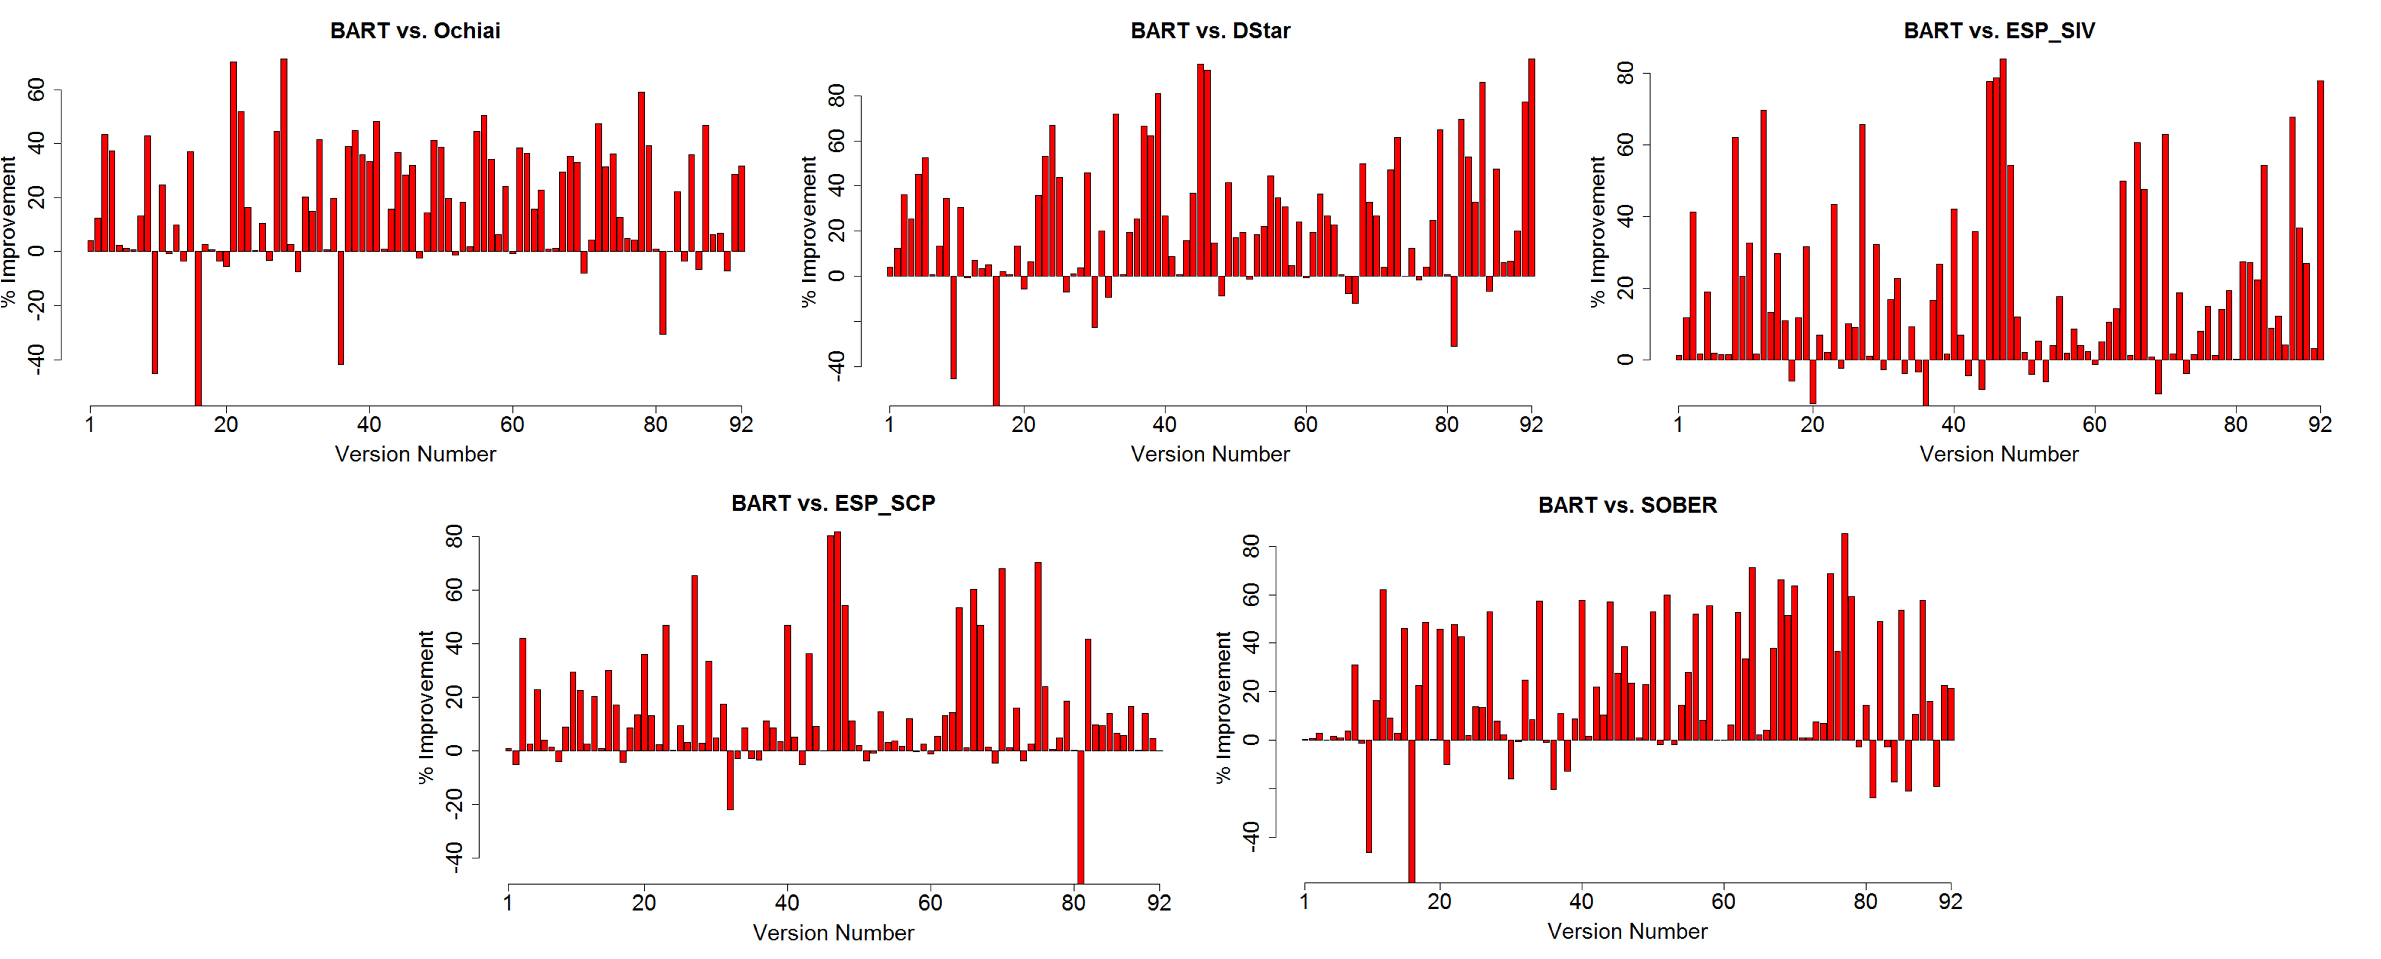
\includegraphics[width=\textwidth]{chapter4_BART_VS_Base.pdf}
\caption{Performance of BART relative to baseline metrics on individual single-fault program versions.}
\label{BART_VS_Base}
\end{sidewaysfigure}

Figure \ref{BART_VS_Base_M} contrasts the performance of BART on the individual two-fault program versions with that of the baseline metrics.  Over all 25 faulty subject-program versions, BART performed better than SOBER on 19 versions but performed worse on 6 versions.  There were 8 versions for which BART performed at least 10\% better than SOBER but 3 versions for which SOBER performed at least 10\% better than BART.  Ochiai performed better than BART on 5 versions but performed worse on 20 versions. BART performed at least 10\% better than Ochiai on 13 versions. BART performed better than both ESP-SIV and ESP-SCP on 20 versions.   BART performed better than DStar on 19 versions.

\begin{sidewaysfigure}
\centering
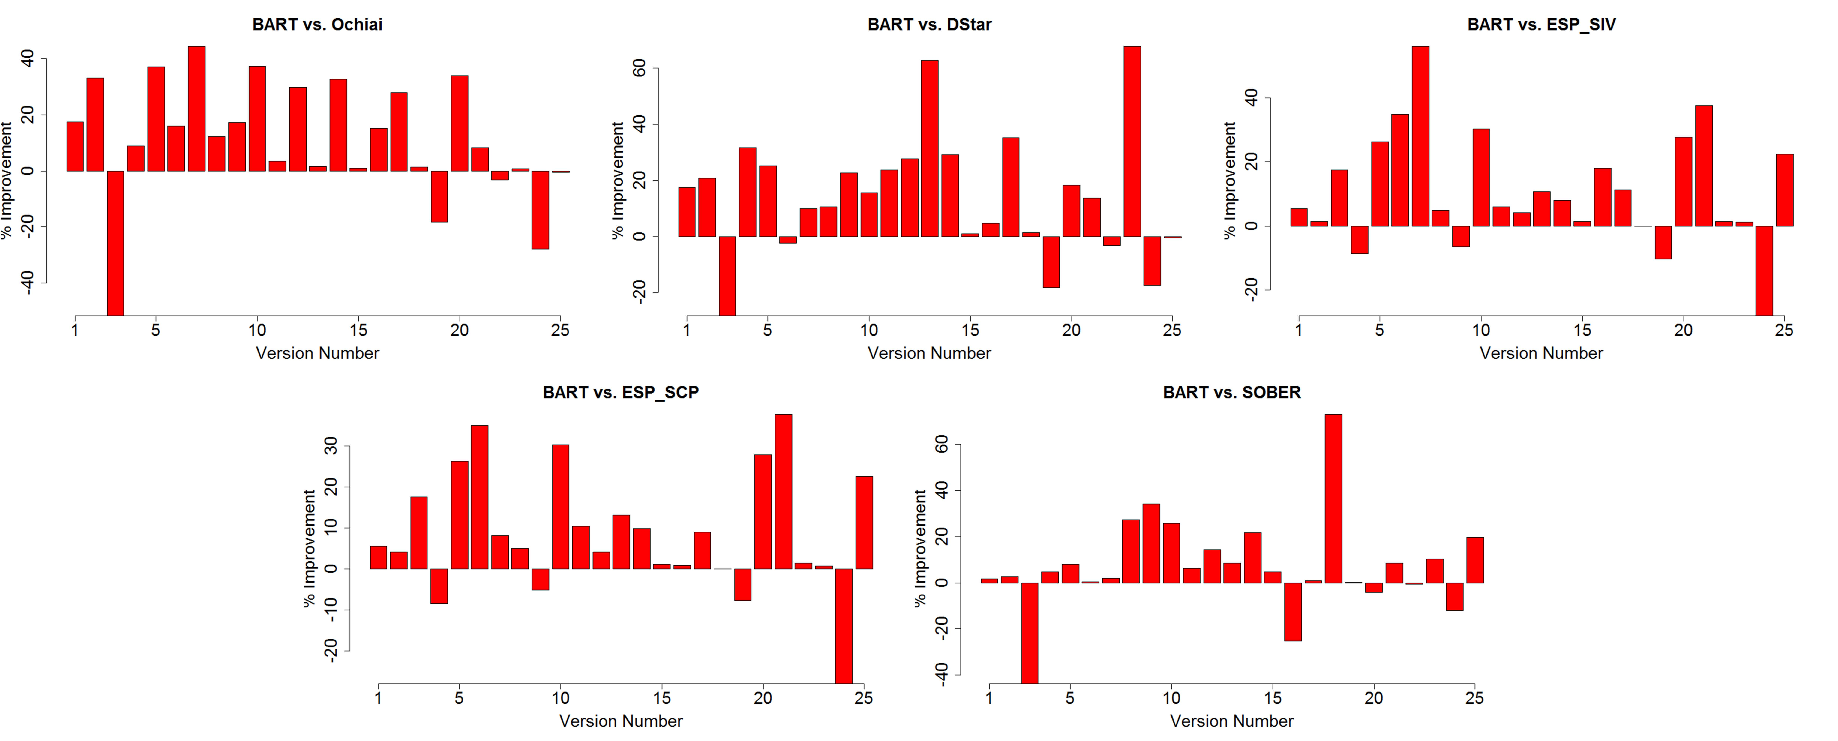
\includegraphics[width=\textwidth]{chapter4_BARTvsBase_M.pdf}
\caption{Performance of BART relative to baseline metrics on individual single-fault program versions.}
\label{BART_VS_Base_M}
\end{sidewaysfigure}


\subsection{BART model vs NUMFL}
Table \ref{tableBARTvsNUMFL} shows the average percentage of subexpressions that had to be examined to find the fault, computed across all the faulty versions, for BART model and NUMFL.  Here we show the results for NUMFL-GPS-QRM and NUMFL-CBPS-QRM.   There were 11 subject programs for which BART performed better than NUMFL-GPS-QRM. There were 5 subject programs for which NUMFL-GPS-QRM performed better than BART. BART performed better than NUMFL-CBPS-QRM on 14 subject programs. There were only 2 subject programs for which NUMFL-CBPS-QRM performed better than BART.

Figure \ref{BARTvsQRM} graphically contrasts the performance of BART and NUMFL-GPS-QRM on the single fault versions.  BART performed better than NUMFL-GPS-QRM on 54 versions, while NUMFL-GPS-QRM performed better on 38 versions.  BART performed at least 20\% better than NUMFL-GPS-QRM on 9 versions, whereas NUMFL-GPS-QRM performed at least 20\% better than BART on 6 versions. Figure \ref{BARTvsCBPS} graphically contrast the performance of BART and NUMFL-CBPS-QRM on the single fault versions.  BART performed better than NUMFL-CBPS-QRM on 61 versions, while NUMFL-CBPS-QRM performed better on 31 versions.  BART performed at least 20\% better than NUMFL-CBPS-QRM on 17 versions, whereas NUMFL-CBPS-QRM performed at least 20\% better than BART on just 4 versions.

In summary, BART  performed better than both NUMFL-GPS-QRM and NUMFL-CBPS-QRM on single-fault programs. This may be due to the fitted sum of trees structure of BART model well approximate the DRF of treatment variable and thus have more accurate average cause effect estimation than NUMFL techiniques.

\begin{table*}[htbp!]
\caption{AVERAGE FAULT LOCALIZATION COSTS OF BART AND NUMFL METRICS ON SINGLE-FAULT PROGRAM VERSIONS}
\label{tableBARTvsNUMFL}
\centering
      \begin{tabular}{|l|c|c|c|}
      \hline
\multirow{2}{*}{Subject Program}	& \multirow{2}{*}{BART}&	\multicolumn{2}{|c|}{{\bf NUMFL}}	\\	\cline{3-4}
& & GPS-QRM	&CBPS-QRM \\ \hline
Apache\_EigenDecompose &	2.50\%&	12.3\%	&	8.8\%	\\	\hline
Apache\_DScompiler&	9.72\%&	11\%	&	12\%	\\	\hline
Apache\_BigMatrix	&	9.00\%&11.4\%	&	9.9\%	\\	\hline
Apache\_Rotation3D&	9.07\%&	8\%	&	18.9\%	\\	\hline
Ojaljo\_SchurDecompose&	10.61\%&	11.4\%	&	14\%	\\	\hline
Jama\_MatrixDecompose	&11.62\%&	14.2\%	&	23\%	\\	\hline
SciMark\_LU&8.33	\%&	15.3\%	&	27.8\%	\\	\hline
SciMart\_FFT&	 27.59\%&	9.5\%	&	19.8\%	\\	\hline
Apache\_SymmLQ&	 1.75\%&	2.6\%	&	4.4\%	\\	\hline
Apache\_SplineInterpolator&	 37.78\%&	31.7\%	&	35\%	\\	\hline
Apche\_SimpleRegress&	 1.70\%&	4.3\%	&	17\%	\\	\hline
Apache\_SchurTransformer&	 4.56\%&	3.3\%	&	14.9\%	\\	\hline
Apache\_MillerUpdatRegress&	 1.24\%&	7.5\%	&	9.9\%	\\	\hline
Apache\_HarmonicFitter&	30.10\%&	27.3\%	&	32\%	\\	\hline
Apache\_FastSine&	1.53\%&	1.5\%	&	13\%	\\	\hline
Apache\_FastCosine	&1.29	\%&1.3\%	&	1.2\%	\\	\hline
Average Cost	&	10.52\%&10.8\%	&	16.4\%	\\	\hline
\end{tabular}
\end{table*}

\begin{figure*}[!thpb]
\centering
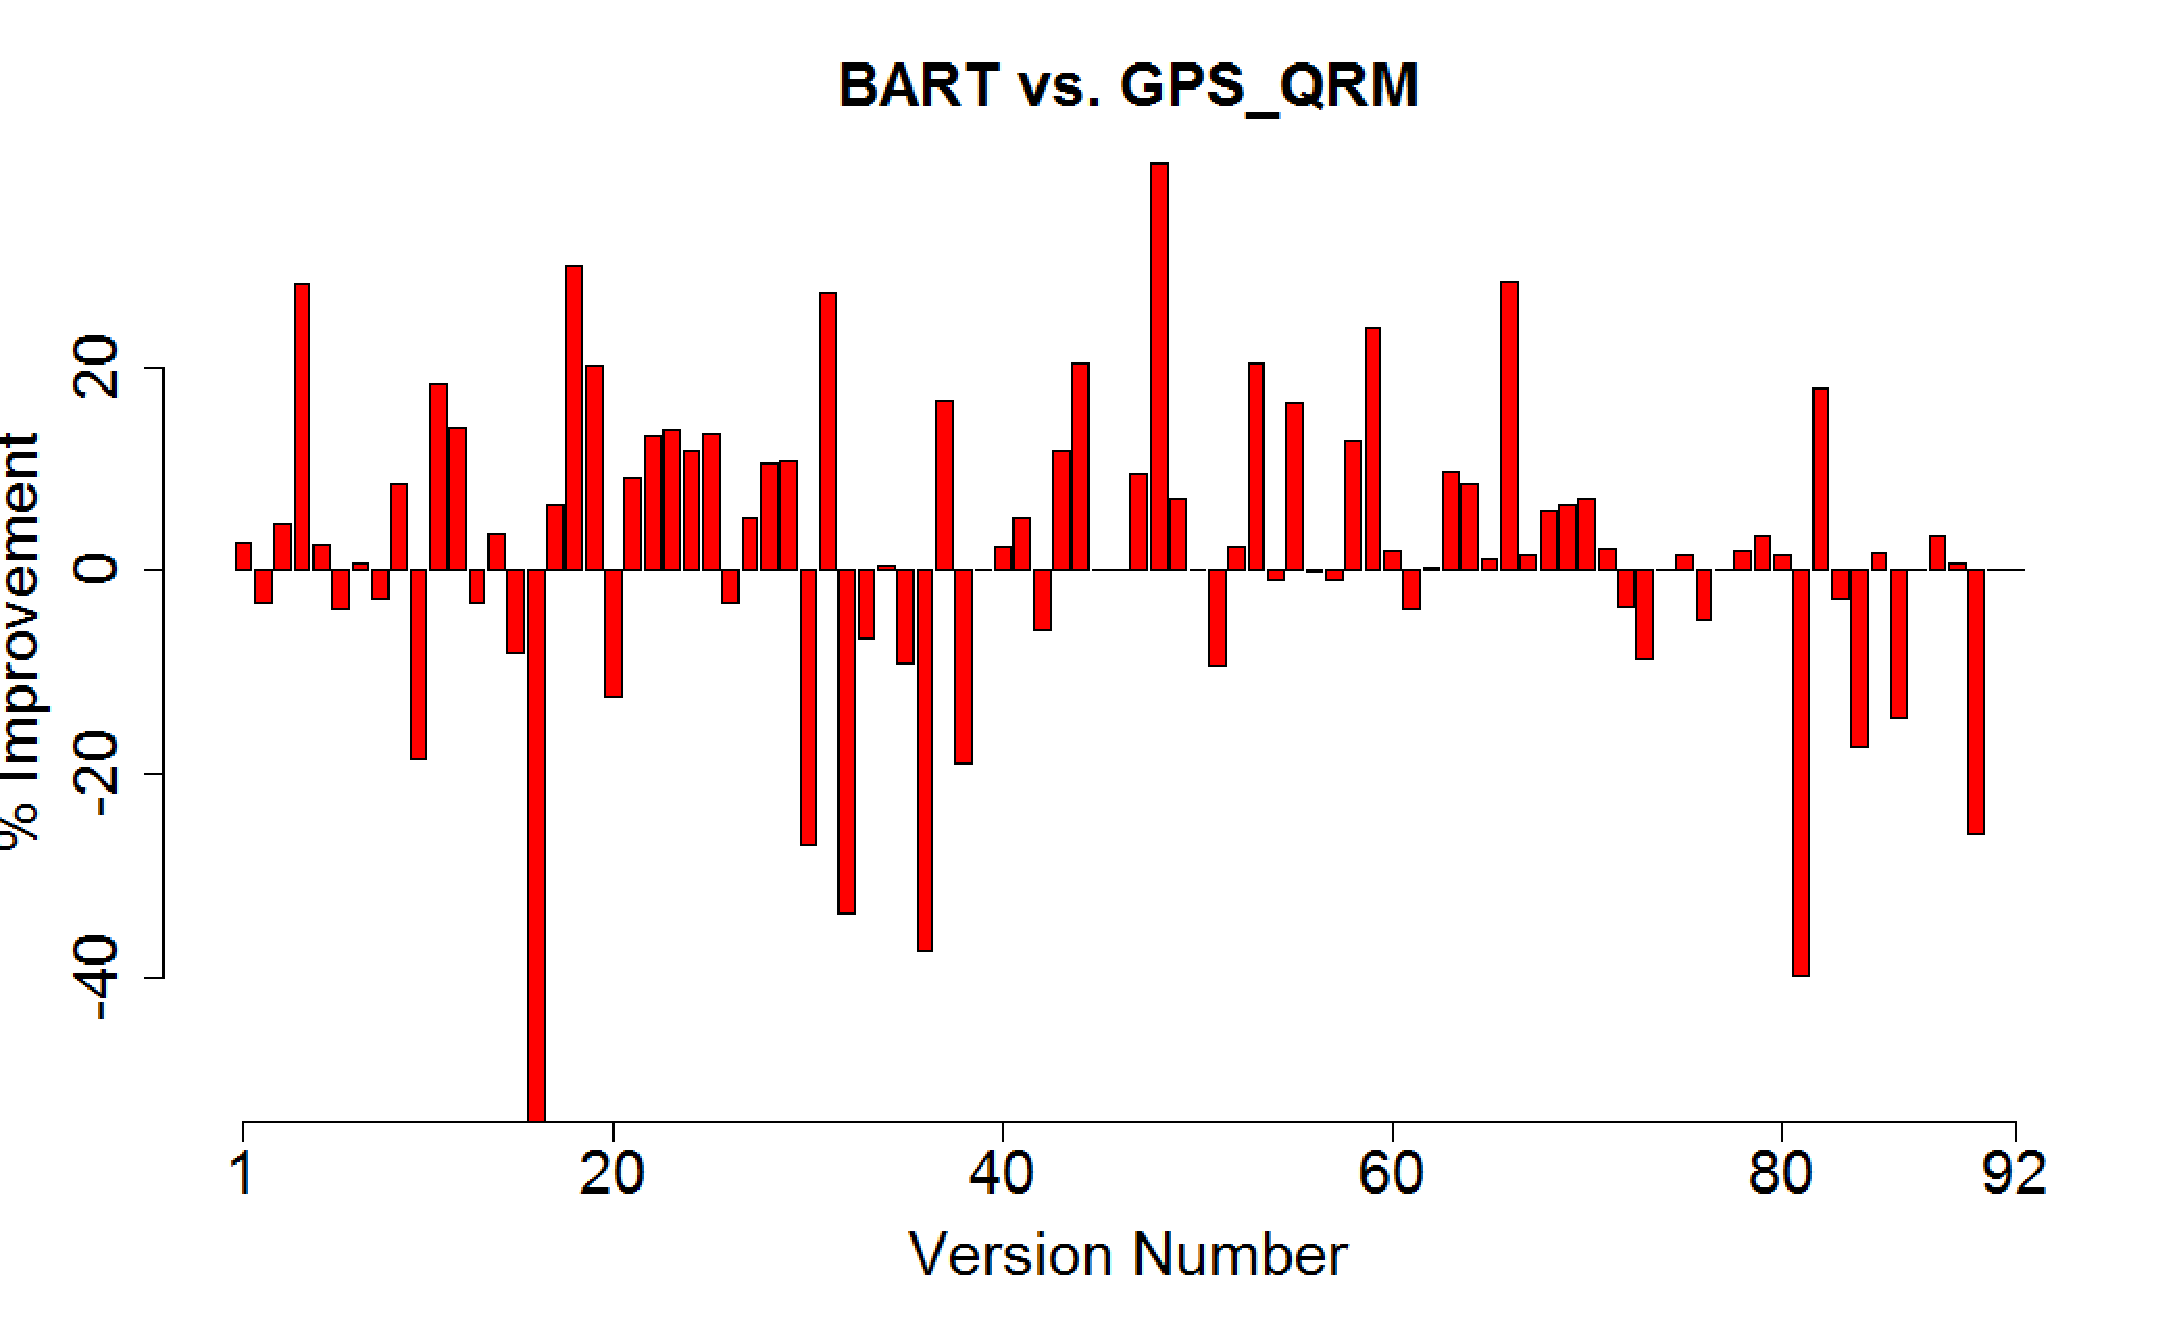
\includegraphics[width=0.8\textwidth]{chapter4_BARTvsGPS_QRM.pdf}
\caption{Relative performance of NUMFL-GPS-QRM with and without data from passing runs, on individual single-fault program versions.}
\label{BARTvsQRM}
\end{figure*}

\begin{figure*}[!thpb]
\centering
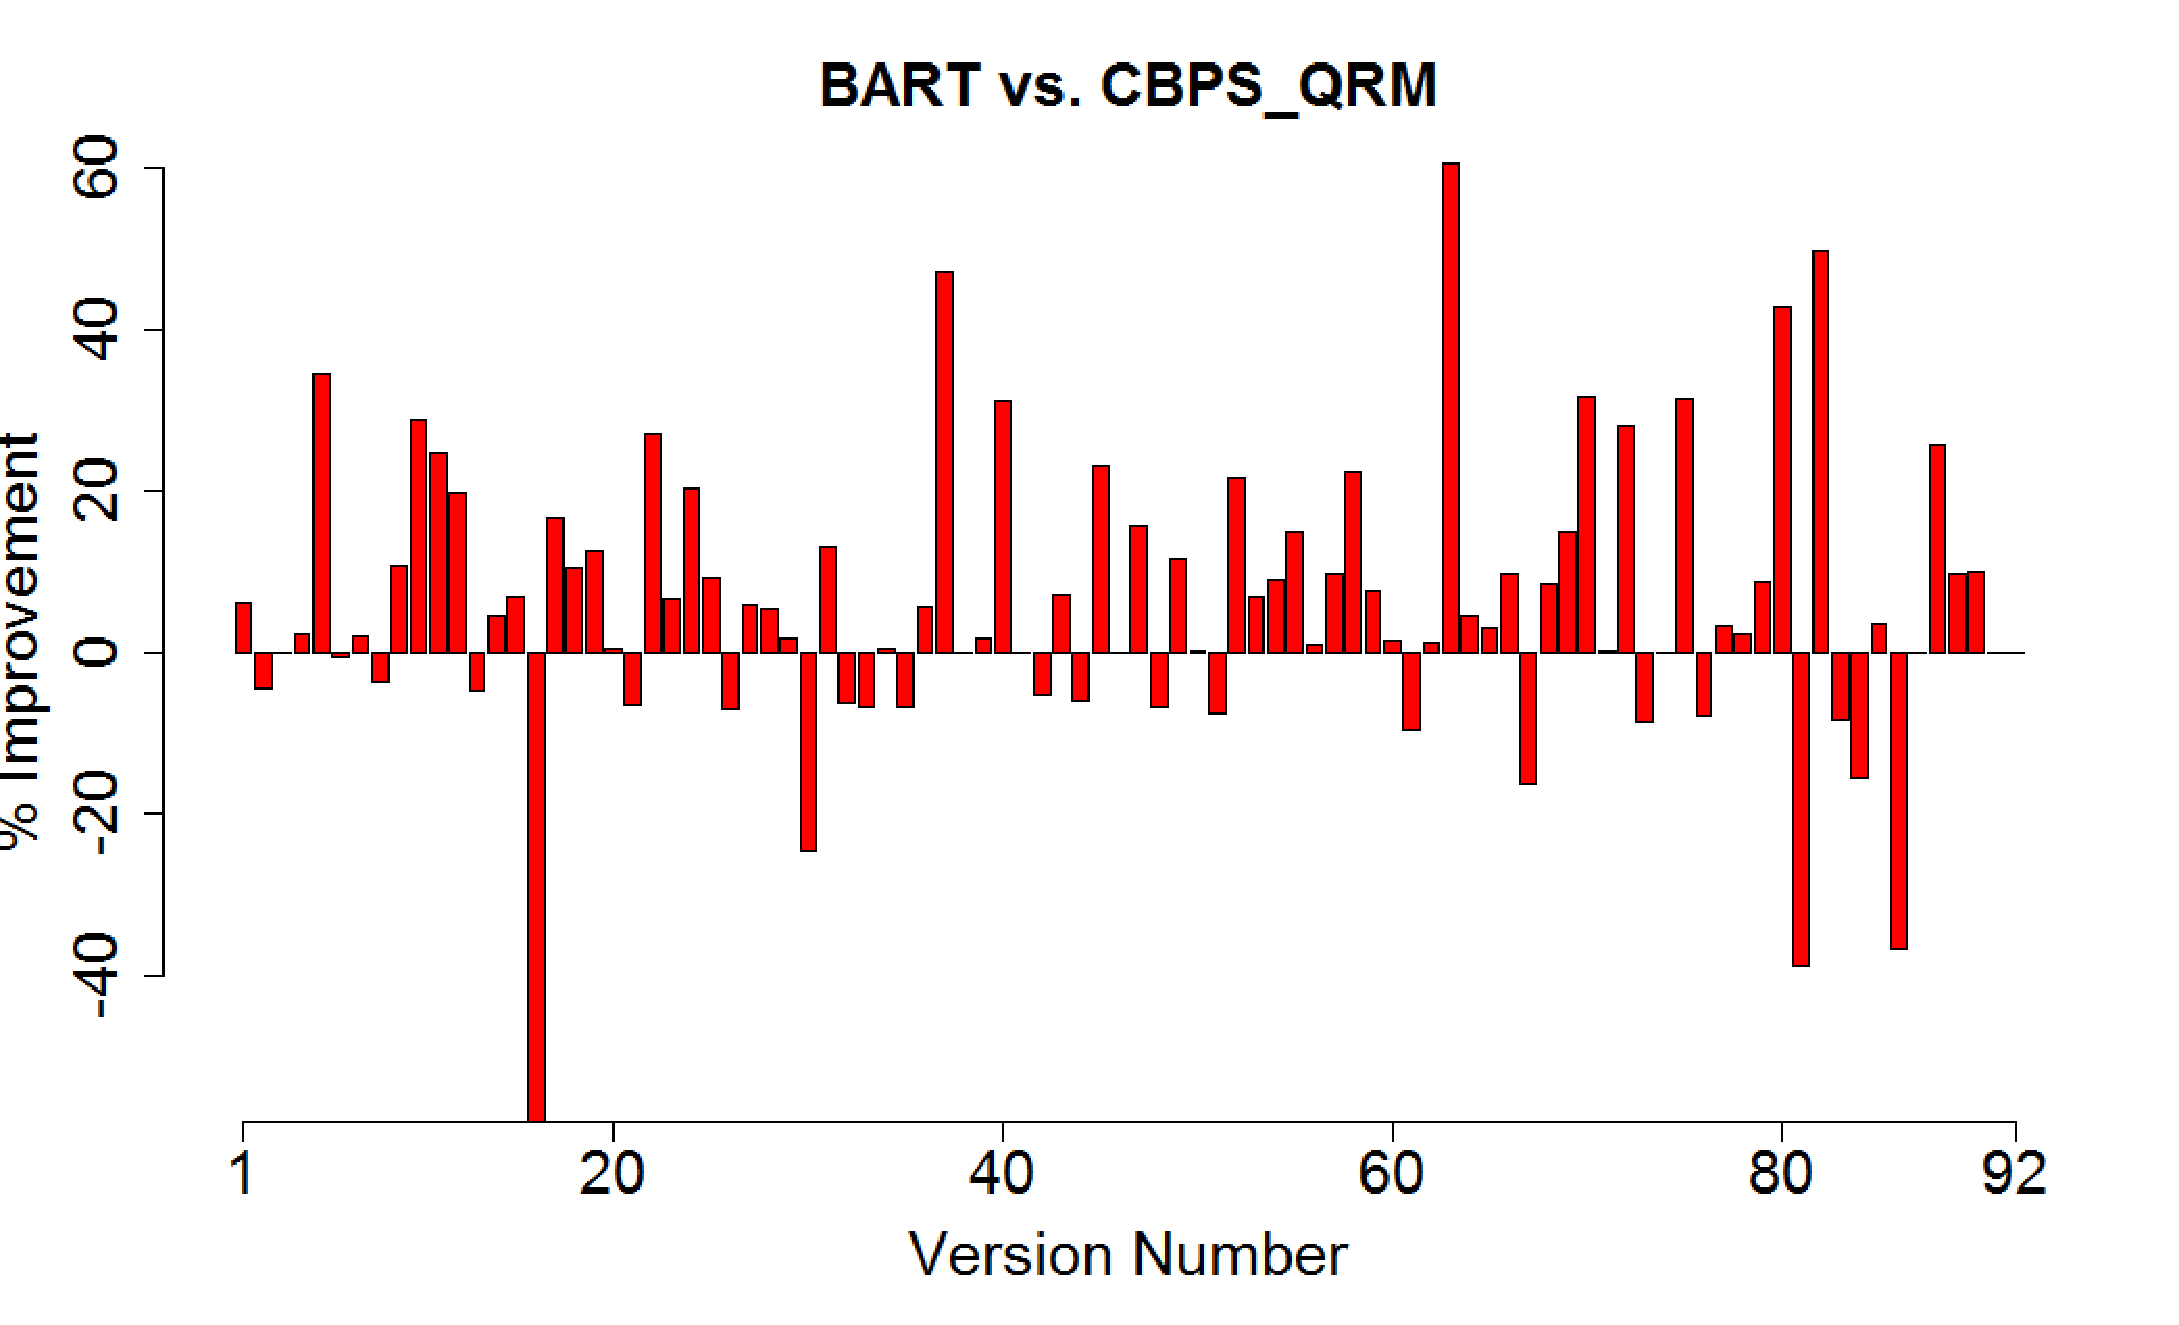
\includegraphics[width=0.8\textwidth]{chapter4_BARTvsCBPS.pdf}
\caption{Relative performance of NUMFL-GPS-QRM with and without data from passing runs, on individual single-fault program versions.}
\label{BARTvsCBPS}
\end{figure*}

Table \ref{tableBARTvsNUMFL_M} shows the average cost, over the faulty versions of each subject program into which two faults were injected, of localizing the first fault to be found, for both BART and NUMFL.  From Table \ref{tableBARTvsNUMFL_M}, the average cost of BART is close to that of NUMFL-GPS-QRM on two faults subject programs. BART performed better than NUMFL-GPS-QRM on the versions of  2 subject programs, but performed worse than NUMFL-GPS-QRM on the versions of 3 subject program.  BART performed better than NUMFL-CBPS-QRM on the versions of 4 subject programs, but performed worse than NUMFL-CBPS-QRM on the versions of only 1 subject program.

Figure \ref{BARTvsGPS_M} graphically contrasts the performance of the BART and NUMFL-GPS-QRM on the individual two-fault versions.  BART performed better than NUMFL-CBPS-QRM on 13 versions and NUMFL-GPS-QRM performed worse on 12 versions.  BART performed at least 10\% better than NUMFL-GPS-QRM on 7 versions, whereas NUMFL-CBPS-QRM performed at least 10\% better than NUMFL-GPS-QRM on just 1 version. Figure \ref{BARTvsCBPS_M} graphically contrasts the performance of the BART and NUMFL-CBPS-QRM on the individual two-fault versions.  BART performed better than NUMFL-CBPS-QRM on 13 versions and NUMFL-CBPS-QRM performed worse on 12 versions.  BART performed at least 10\% better than NUMFL-CBPS-QRM on 7 versions, whereas NUMFL-CBPS-QRM performed at least 10\% better than NUMFL-GPS-QRM on just 1 version.

\begin{table*}[htbp!]
\caption{AVERAGE FAULT LOCALIZATION COSTS OF BART AND NUMFL ON MULTIPLE-FAULT PROGRAM VERSIONS}
\label{tableBARTvsNUMFL_M}
\centering
      \begin{tabular}{|l|c|c|c|}
      \hline
\multirow{2}{*}{Subject Program}	& \multirow{2}{*}{BART}&	\multicolumn{2}{|c|}{{\bf NUMFL}}	\\	\cline{3-4}
& & GPS-QRM	&CBPS-QRM \\ \hline
Apache\_EigenDecompose	&7.98	\%&10.3\%	&	11.1\%	\\	\hline
Apache\_DScompiler	&	5.13\%&4.5\%	&	5.9\%	\\	\hline
Apache\_Rotation3D	&	10.69\%&7.0\%	&	3.0\%	\\	\hline
Ojaljo\_SchurDecompose	&17.55	\%&5.4\%	&	19.8\%	\\	\hline
Jama\_MatrixDecompose	&	4.65\%&14.1\%	&	23.4\%	\\	\hline
{\bf Average Cost} &9.20\% &8.26\% &12.64\%\\ \hline
\end{tabular}
\end{table*}

\begin{figure*}[!thpb]
\centering
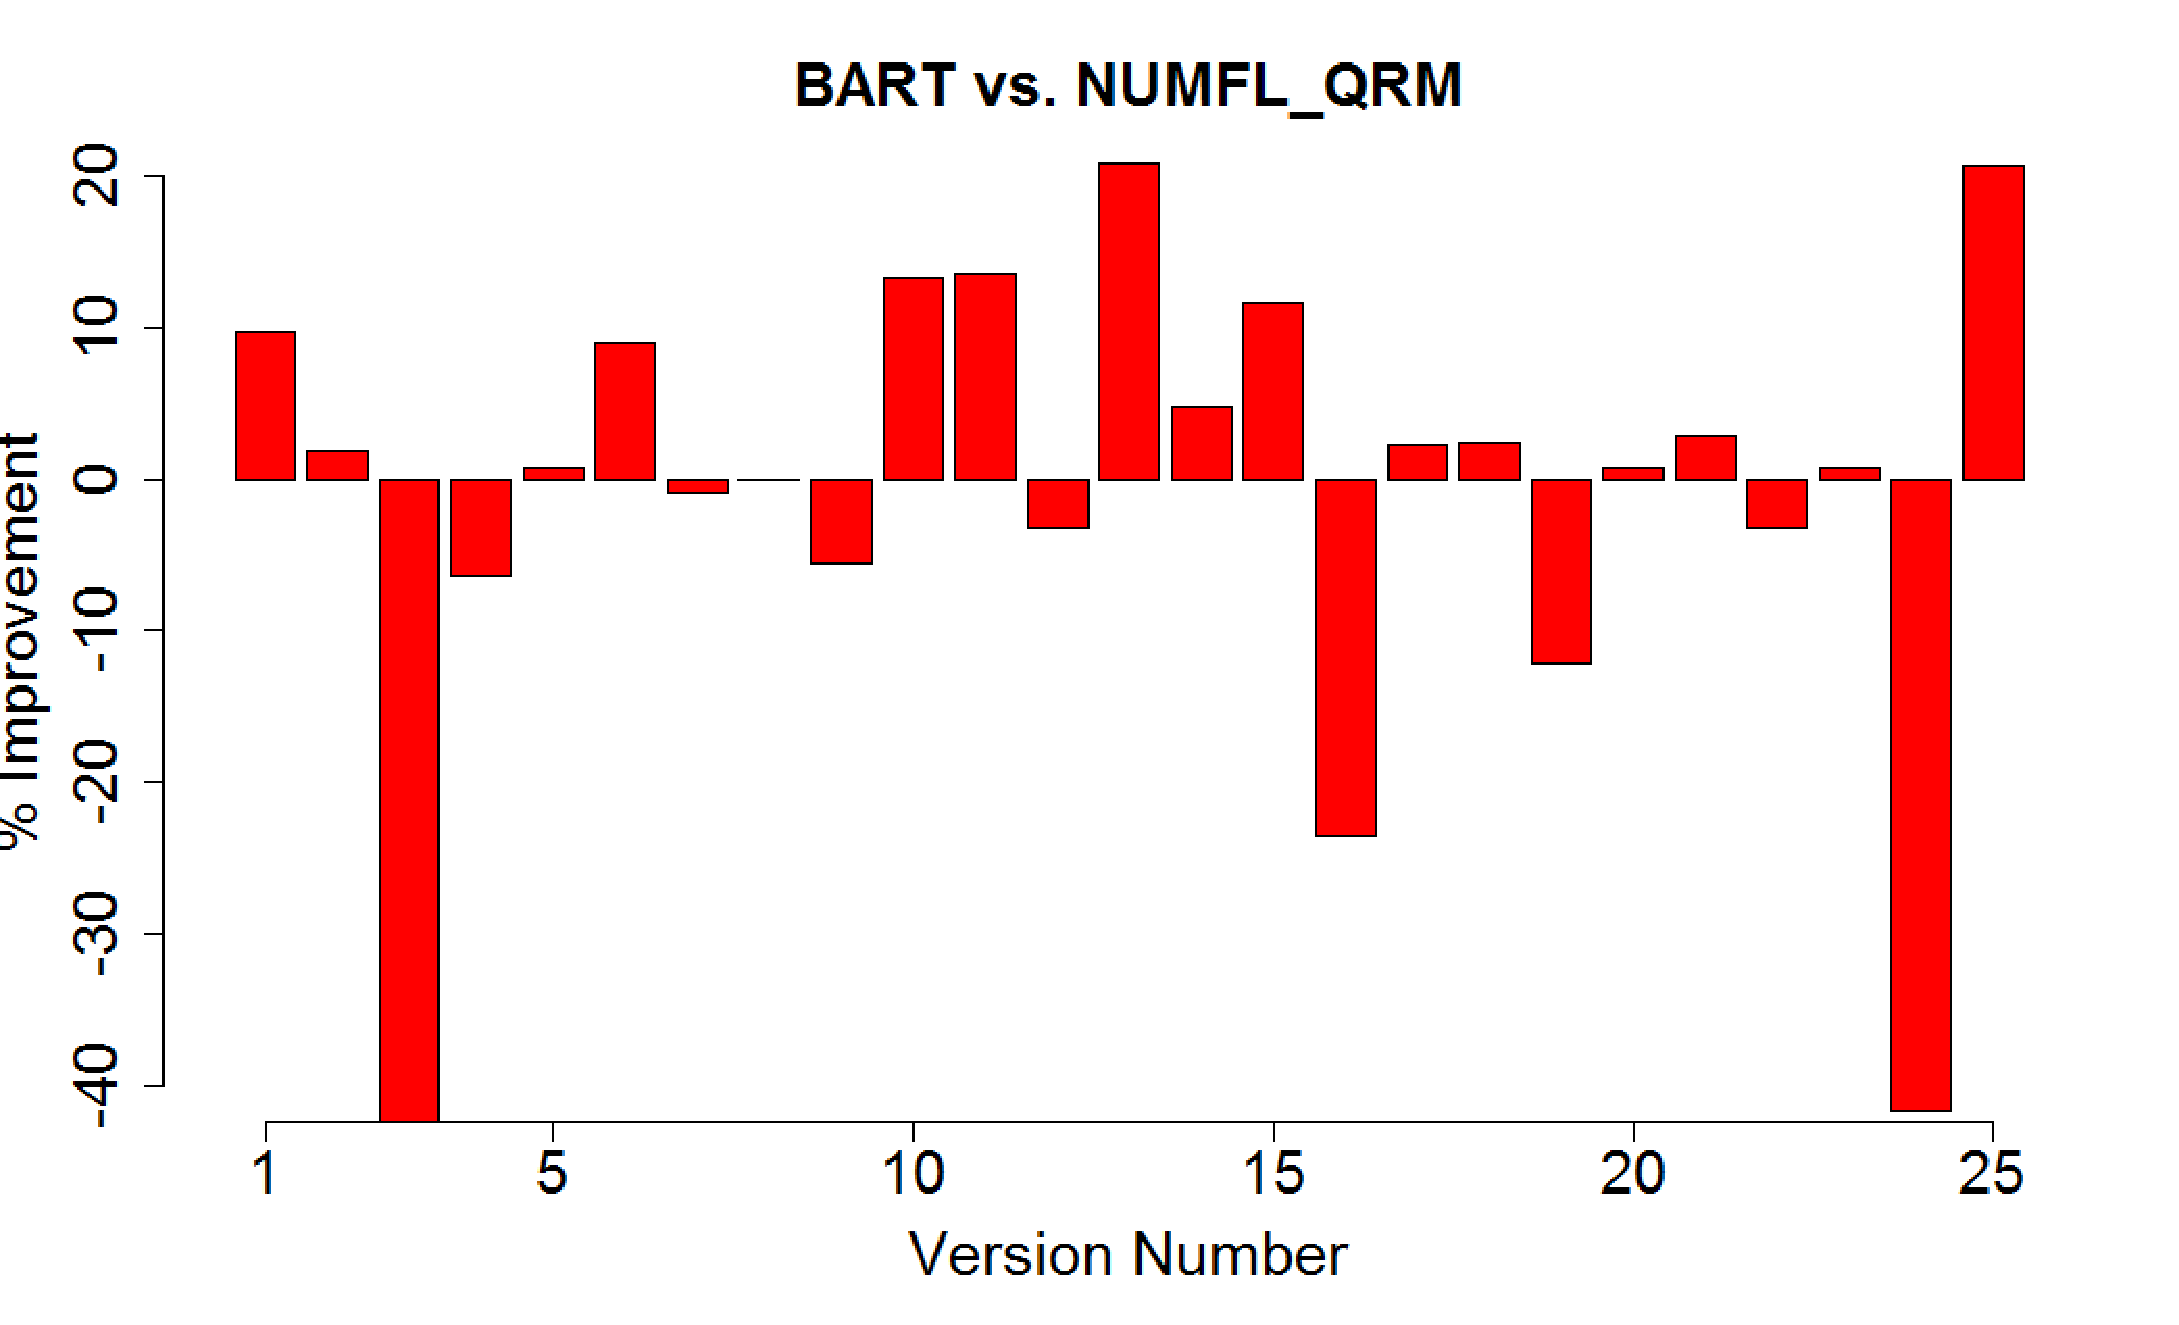
\includegraphics[width=0.8\textwidth]{chapter4_BARTvsGPS_QRM_M.pdf}
\caption{Relative performance of NUMFL-GPS-QRM with and without data from passing runs, on individual single-fault program versions.}
\label{BARTvsGPS_M}
\end{figure*}

\begin{figure*}[!thpb]
\centering
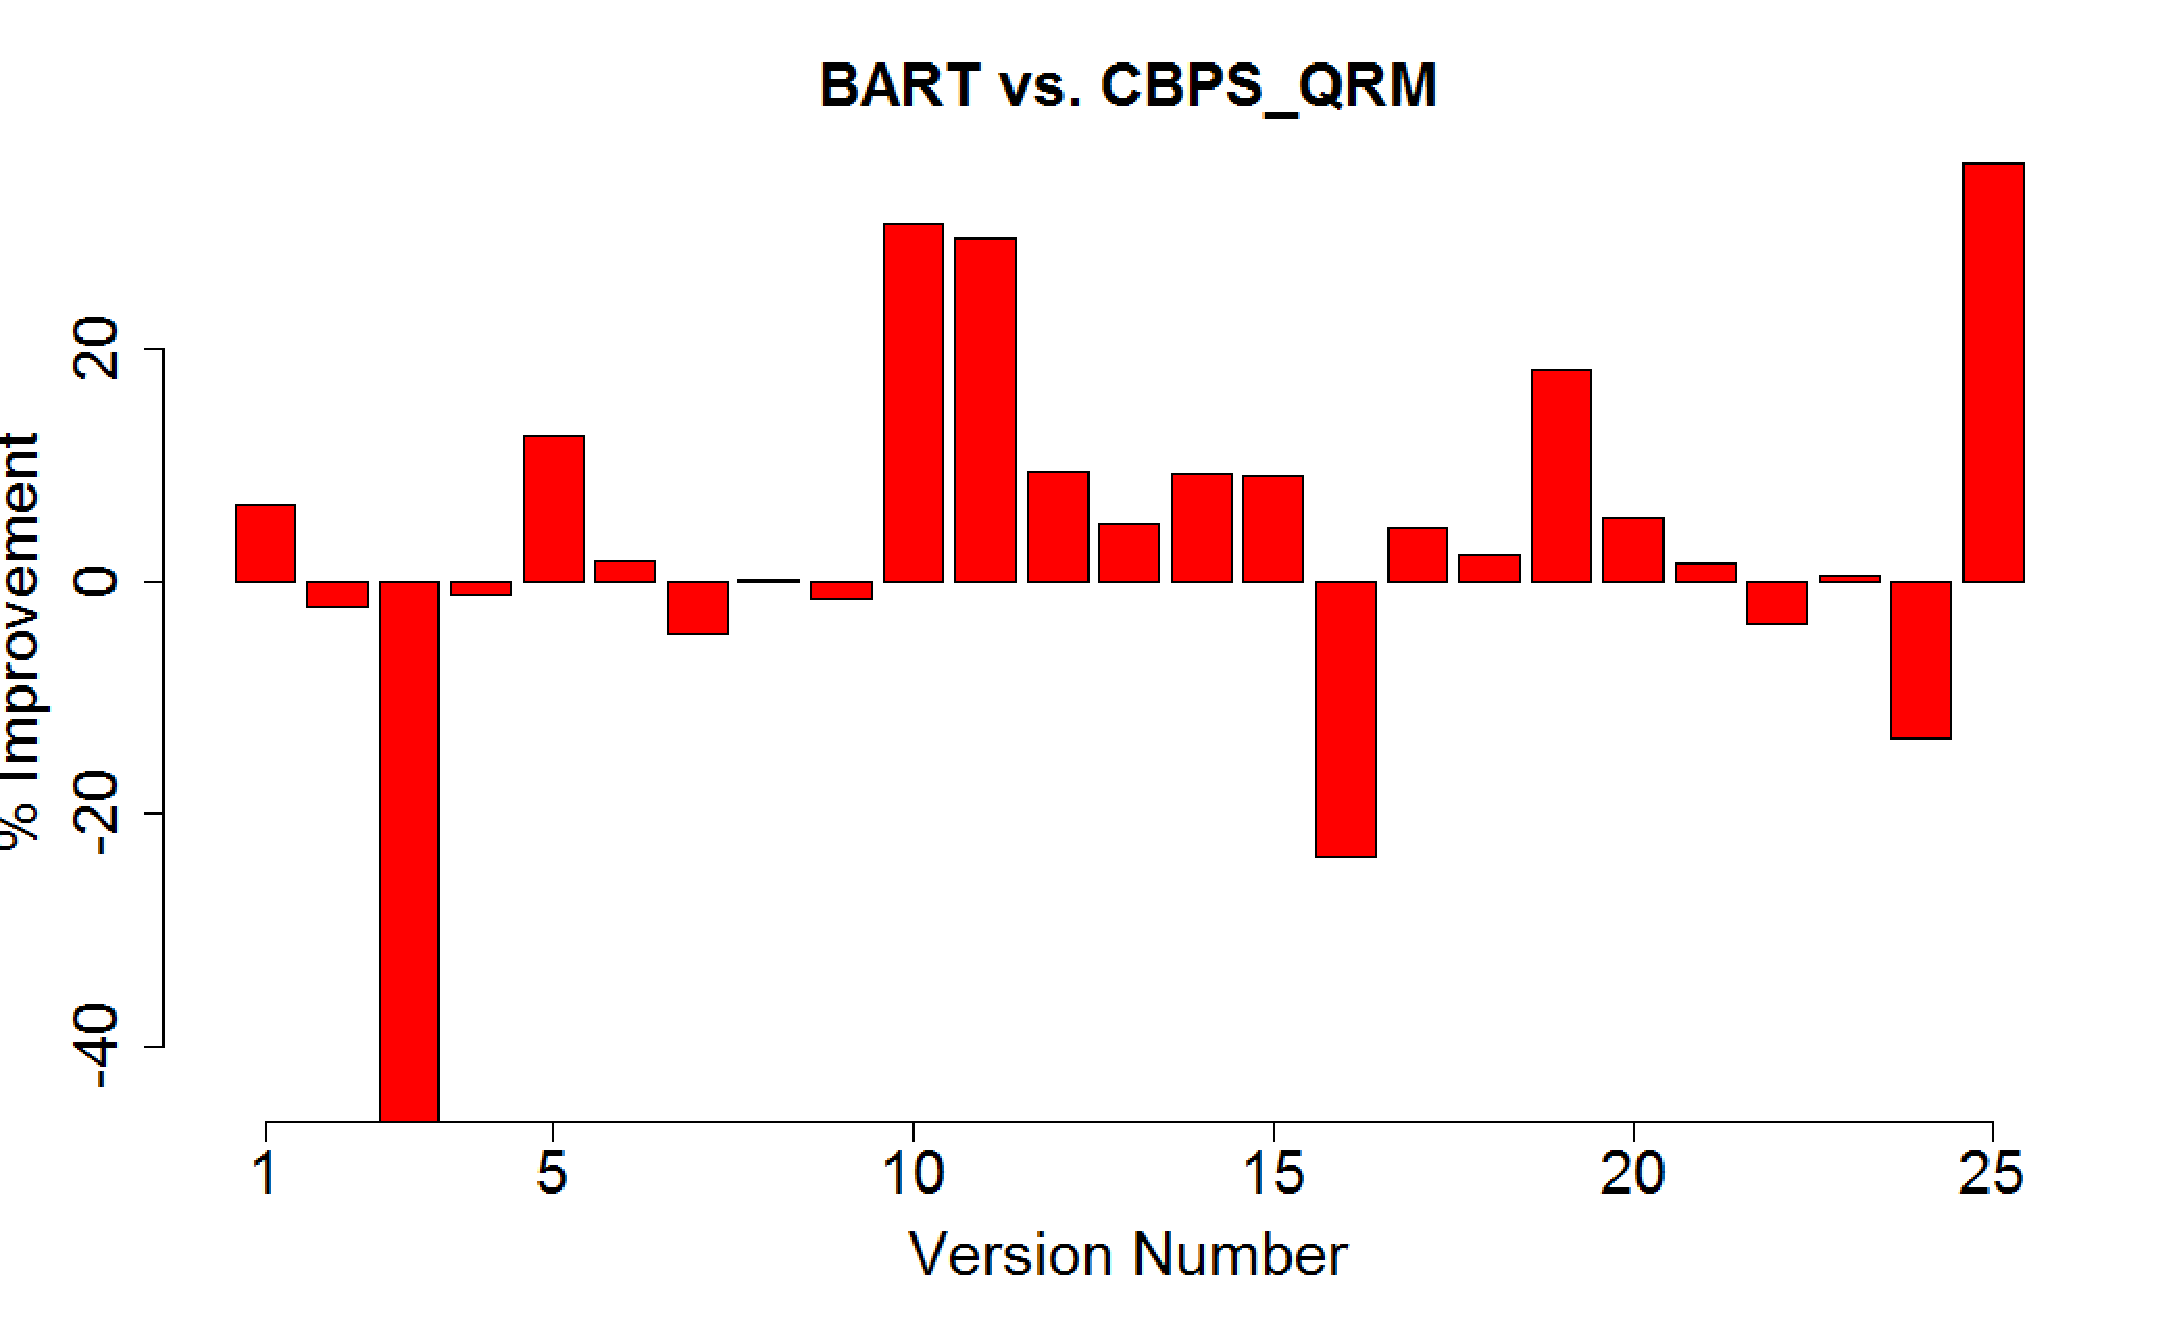
\includegraphics[width=0.8\textwidth]{chapter4_BARTvsCBPS_M.pdf}
\caption{Relative performance of NUMFL-GPS-QRM with and without data from passing runs, on individual single-fault program versions.}
\label{BARTvsCBPS_M}
\end{figure*}

\subsection{Sensitivity of BART model on the number of trees and number of tests}\label{BARTsensitivity}

In previous sections, we use the full observational data of tests to fit a BART model with 10 trees in the sum of trees structure. In this section, we will analyze if increasing number of trees or decreasing the number of tests would influence the performance of BART. In Table \ref{sensitivity}, the first column of numbers is the fault localization cost of BART model contains 10 trees and fitted with full observational data (3000-8000 tests). The second column of numbers is the fault localization cost of BART model contains 50 trees and fitted with full observational data. The third column of numbers is the fault localization cost of BART model contains 10 trees but fitted with only 300 tests' data. From Table \ref{sensitivity}, when increased the number of trees from 10 to 50, BART model has better performance on 6 subject programs. But there are also 6 subject program where BART model's performance become worse after increasing the number of trees. The average cost across 16 subject programs is roughly same: 10.52\% for BART model with 10 trees and 10.58\% for BART model with 50 trees. This means 10 trees are enough to handle the nonlinearity problem in AFCE estimation.  When decrease the number of tests to 300, the average cost is slightly increased to 10.74\%.  This means BART model does not require a large number of tests to localize bugs in numerical software.

\begin{table*}[htbp!]
\caption{AVERAGE FAULT LOCALIZATION COSTS OF BART MODEL WITH DIFFERENT NUMBER OF TREES AND TESTS ON ONE SINGLE-FAULT PROGRAM VERSIONS }
\label{sensitivity}
\centering
      \begin{tabular}{|l|c|c|c|}
      \hline
\multirow{2}{*}{{\bf Subject Program}}	&	\multicolumn{3}{|c|}{{\bf BART Model}}	\\	\cline{2-4}
& 10 trees & 50 trees & 300 tests\\ \hline
Apache\_EigenDecompose			&	2.50	\%	&	3.07	\%	&	2.38	\%	\\ \hline
Apache\_DScompiler			&	9.72	\%	&	8.61	\%	&	9.64	\%	\\ \hline
Apache\_BigMatrix			&	9.00	\%	&	9.05	\%	&	9.00	\%	\\ \hline
Apache\_Rotation3D			&	9.07	\%	&	8.73	\%	&	8.16	\%	\\ \hline
Ojaljo\_SchurDecompose			&	10.61	\%	&	9.89	\%	&	11.44	\%	\\ \hline
Jama\_MatrixDecompose			&	11.62	\%	&	11.16	\%	&	11.32	\%	\\ \hline
SciMark\_LU			&	8.33 \%	&	9.72	\%	&	6.94	\%	\\ \hline
SciMart\_FFT			&	27.59	\%	&	26.72	\%	&	27.59	\%	\\ \hline
Apache\_SymmLQ			&	1.75	\%	&	1.75	\%	&	1.75	\%	\\ \hline
Apache\_SplineInterpolator			&	37.78	\%	&	40	\%	&	45.56	\%	\\ \hline
Apche\_SimpleRegress			&	1.70	\%	&	1.70	\%	&	1.70	\%	\\ \hline
Apache\_SchurTransformer			&	4.56	\%	&	4.88	\%	&	4.23	\%	\\ \hline
Apache\_MillerUpdatRegress			&	1.24	\%	&	1.24	\%	&	1.24	\%	\\ \hline
Apache\_HarmonicFitter			&	30.10	\%	&	30.08	\%	&	28.06	\%	\\ \hline
Apache\_FastSine			&	1.53	\%	&	1.53	\%	&	1.53	\%	\\ \hline
Apache\_FastCosine			&	1.29	\%	&	1.29	\%	&	1.29	\%	\\ \hline
Average Cost 	&	10.52\% 	&10.58\% 	&10.74\%	\\ \hline
\end{tabular}
\end{table*}

\subsection{Computation Time Analysis}
In this study, we use a Dell Precision T5600 with two 2.30 GHz intel Xeon CPUs and 64 GB RAM. Table \ref{BARTcomputetime} summarized the average computation time of the three BART models described in last section on each subject program.  When the number of trees increased from 10 to 50, the average computation cost nearly doubled. If we reduced number the tests from more than 3000 to 300, the computation cost will reduced more than 50\%.  From Table \ref{BARTcomputetime} and Table \ref{sensitivity}, we can conclude that the BART model with 10 trees and fitted with 300 tests get the best cost-performance ratio among the three BART models fitted with different settings. But we also need to point out that even the BART model is fitted with 300 tests, its computation cost is still about twice of the computation cost of NUMFL. Thus, the computation cost is a weakness of applying BART model on localizing faults in numerical programs. 

\begin{table*}[htbp!]
\caption{AVERAGE COMPUTATION TIME OF NUMFL-GPS-QRM AND NUMFL-CBPS-QRM ON ONE SINGLE-FAULT PROGRAM VERSIONS }
\label{BARTcomputetime}
\centering
      \begin{tabular}{|l|c|c|c|}
      \hline
\multirow{2}{*}{{\bf Subject Program}}	&	\multicolumn{3}{|c|}{Average Computation Time (Secs)}	\\	\cline{2-4}
& 10 trees & 50 trees & 300 tests\\ \hline

Apache\_EigenDecompose	&	2856.73	&	5530.20	&	1205.97	\\ \hline
Apache\_DScompiler	&	628.31	&	1243.78	&	274.88	\\ \hline
Apache\_BigMatrix	&	696.58	&	1337.73	&	292.28	\\ \hline
Apache\_Rotation3D	&	2668.41	&	5550.45	&	1082.64	\\ \hline
Ojaljo\_SchurDecompose	&	2636.96	&	5013.37	&	1313.53	\\ \hline
Jama\_MatrixDecompose	&	3134.49	&	6005.71	&	1262.88	\\ \hline
SciMark\_LU	&	167.94	&	332.45	&	121.38	\\ \hline
SciMart\_FFT	&	393.26	&	842.31	&	234.09	\\ \hline
Apache\_SymmLQ	&	908.12	&	1986.32	&	245.21	\\ \hline
Apache\_SplineInterpolator	&	364.80	&	747.42	&	135.00	\\ \hline
Apche\_SimpleRegress	&	823.34	&	1685.88	&	227.27	\\ \hline
Apache\_SchurTransformer	&	768.44	&	1539.44	&	315.65	\\ \hline
Apache\_MillerUpdatRegress	&	396.10	&	808.59	&	198.61	\\ \hline
Apache\_HarmonicFitter	&	326.09	&	673.73	&	120.28	\\ \hline
Apache\_FastSine	&	1006.86	&	2064.98	&	259.78	\\ \hline
Apache\_FastCosine	&	1089.13	&	2229.39	&	294.56	\\ \hline
\end{tabular}
\end{table*}

\section{RELATED WORK}\label{BARTrelatedwork}
The most related works to this study are those using BART model to estimate treatment causal effect. Hill et al. proposed to apply BART model for causal inference and data science \cite{hill2012bayesian, hill2013assessing}. In the paper, they designed the method of using BART to estimate average causal effect of binary treatment variable and discussed how to use BART to handle continuous treatment variables and outcome missing data. Later, Green et al. applied BART to model heterogeneous treatment effects \cite{green2012modeling}. Sparapani et al. extends the usefulness of BART in medical applications by addressing needs arising in survival analysis \cite{sparapani2016nonparametric}.

Another related work is using tree structure in fault localization. Chen et al \cite{chen2004failure} present a decision tree learning approach to identify the causes of failures in internet sites. Francis et al \cite{francis2004tree} use tree based method to classify software failures. Kiciman et al \cite{kiciman2005root} use decision tree to diagnose which component of large scale systems is the root cause of failure. However, unlike our models, all their works do not localize the fault on statement level.

\section{CONCLUSION}\label{BARTconclusion}
BART model is a Bayesian non-parametric model which can capture both nonlinearities and interactions between variables without knowing the information about how these variables are parametrically related . BART uses a sum of trees structure to approximate the dose response function of continuous treatment variables. The AFCE can be estimated by averaging the causal effect of treatment on outcome at each observation unit. We reported the result of an empirical comparison of BART model to several competing fault localization metrics on both single-fault subject programs and multiple-fault subject programs. BART model performed significantly better than the other techniques. We also compare the BART model with NUMFL, which is introduced in chapter 3. The result shows BART model outperforms NUMFL on single faults localization. In multiple faults localization, BART and NUMFL has similar performances.  We also study the sensitivity of the BART model to the number of trees and the number of tests. The result shows BART is robust on the sample size and number of trees.   
\chapter{Fault Localization in Embedded Control System Software}\label{robot}

\section{Introduction}
Embedded systems are built and used everywhere in modern society. Controllers are the software part of some embedded systems
that control the behavior of the system. For example, consider a robot that has a high level goal of moving from one location to another. Therefore, bug-free control code is an important consideration. Our focus
is on algorithms that can help locate bugs in control code,
therebey reducing development time and improving the safety
of the system.  

Most low-level controllers, including the ones we evaluate, contain very few branch points. Generally, they are sequences of numerical computations that estimate the state of the system, compare to a reference state, solve an
optimal control problem and execute the solution. A bug in this context could be the result of an incorrect mathematical operation in the control code. This means that standard coverage
based fault localization techniques cannot in general be used because essentially the same sequence of statements is executed whether the output is faulty or not. Our prior work on value-based statistical fault localization attempted to develop techniques to locate faults  in numerical software. This is an extremely difficult problem. In this chapter, we focus on a subset of programs, namely embedded control systems. While embedded control systems are ubiquitous, the specific systems that we focus on in our work are robotic surgery systems. Using medical robot control systems, we develop an approach to automatically localize faulty statements in the control code.

The contribution of this chapter is: we implemented a java software with multi-threaded programming to send commands to the robotic surgery system and collect trajectory data; based on previous work, we developed a fault localization algorithm to localize the fault in embedded control system of medical surgery robot. In the following, we first provide additional background for our problem domain. Next, we describe our approach in detail, followed by empirical evaluation. Finally we give an overview of related work and conclude.

\section{Two Medical Surgery Robot Systems }\label{secrobot}
In this study, we use two prototype robotic surgery systems which are developed by Case MeRCIS Lab \cite{}. The first robot is Small Animal Biopsy Robot(SABiR) \cite{}. The second robot is Beating Heart Robot(BHR) \cite{}.

\subsection {SABiR}
SABiR is a five-degree-of-freedom (DOF) parallel robotic manipulator which is designed to take biopsies or deliver therapeutic drugs at targets in live small animal subjects. The robot has high position resolution and can realize dexterous alignment of  the needle before insertion. The desined accuracy of SABir is better than 250${\mu}m$. Figure \ref{sabir} shows an image of SABiR robot. 

The robot consists of a need mechanism held by two 5-bar linkage mechanisms, referred to as the front and rear stages. There are two DOF (up/down, left/right) in the front stage and three DOF (up/down, left/right, rotate forward/rotate backward) in the rear stage. The robot's hardware state is characterized by its five joint angles. The robot’s needle position and direction can be transformed from 5 joint angles using a bijective inverse kinematic function.

\begin{figure*}[!thpb]
\centering
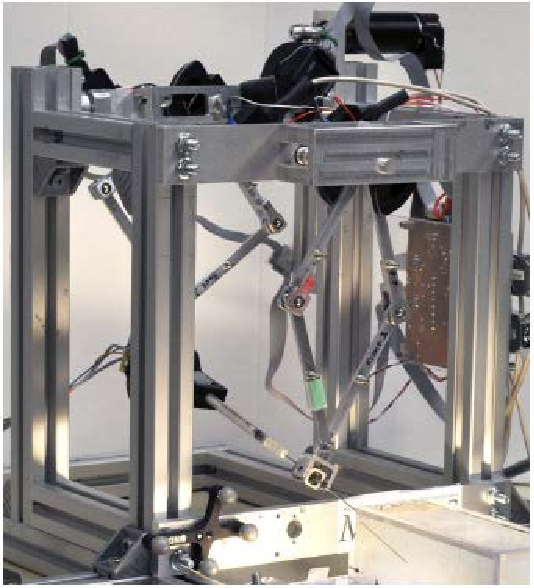
\includegraphics[width=0.6\textwidth]{chapter5_SABiR.pdf}
\caption{SABiR: The robotic system for image-guided needle-based interventions on small animals.}
\label{sabir}
\end{figure*}

\subsection{BHR}
BHR is a manipulator that will allow minimally invasive beating heart surgery. It uses a three DOF robotic platform employing a PHANTom premium 1.5A haptic interface \cite{} as the robotic mechanism. The robot is composed of a base rotation and a four-bar linkage, holding a tool arm. The DOF are driven by three motors: one actuating the base rotation, and two actuating the four-bar linkage in parallel. The joint angles are measured by quadrature encoders. The robot's hardware state is characterized by its three joint angles, and there is a bijective inverse kinematic function to map any position and direction of robot’s end effector to a set of joint angles. Figure \ref{bhr} shows an image of BHR robot.

\begin{figure*}[!thpb]
\centering
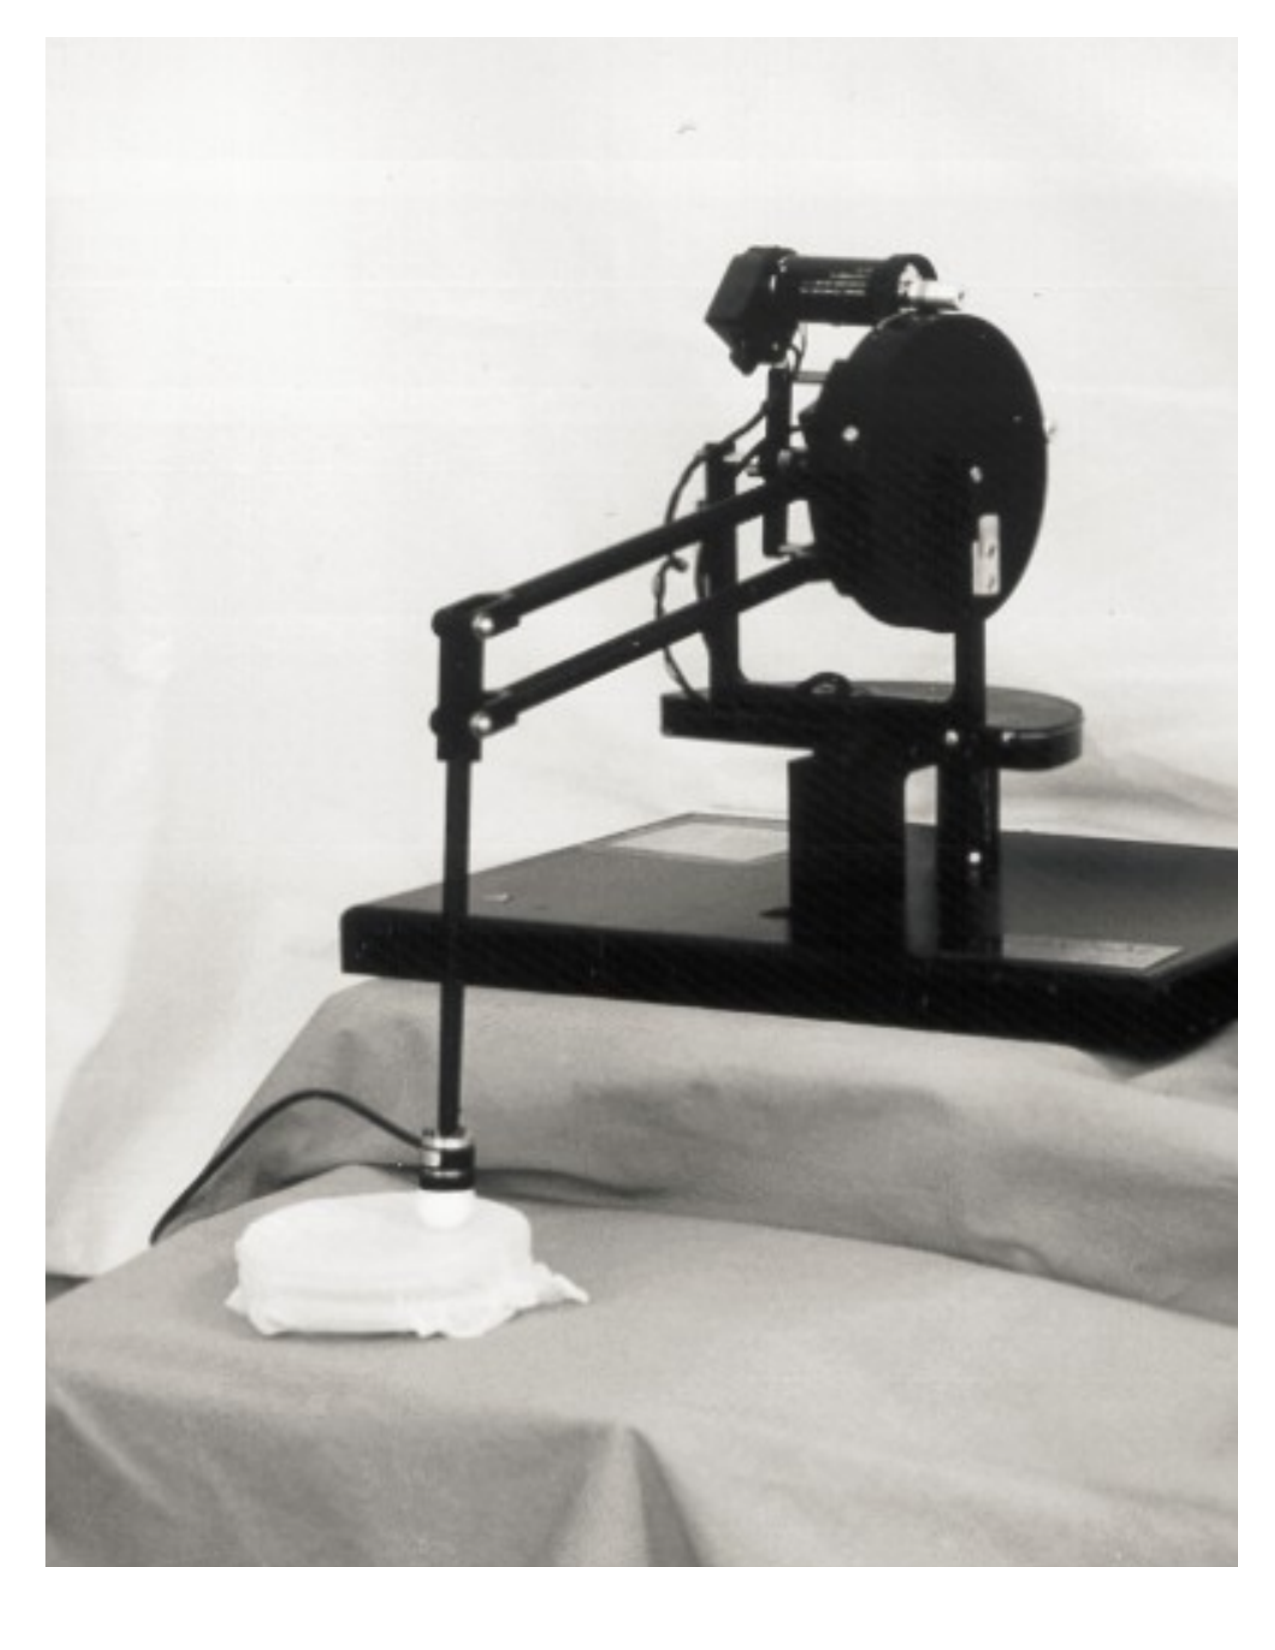
\includegraphics[width=0.6\textwidth]{chapter5_BHR.pdf}
\caption{BHR:Beating Heart Robot}
\label{bhr}
\end{figure*}

\section{Robot Simulation and Control}\label{robotsimulator}
The first part of our framework involves the development of an accurate simulator to ``stand in'' for the actual robot. 

For SABiR we have developed models for the kinematics and inverse kinematics for this robot~\cite{hwang2009kinematic} in prior work. We use these to create a simulation of the robot, implemented in Simulink, in which the robot's motors are each represented as third-order transfer functions. The simulator is designed to be a modular component of the system, in the sense that it can be seamlessly swapped with the controller of the actual robot.

The environment simulation mainly contains two parts. The first part is two gel blocks to simulate the "tissue" in the workspace of the robot.  The second part is a needle force model to simulate the resisive force caused by the combined frictional, cutting, and stiffness forces produced when the needle is inside the gel block. The cutting force is caused by the needletip piercing the gel block and provides a resistance to the needle's motion during insertion into the gel block.  The frictional force is produced by the friction between the needle body and the walls of the channel in the gel block, and resists the needle during insertion and extraction. The stiffness force is caused by the gel block's tendency to resist sideways motion of the needle, i.e., any motion not in the direction the needle is pointing. In this way, realistic and distinguishable forces can be produced by any possible motion of the needle. The needle model is described in detail in~\cite{Russell2012}.

We use a simple low level controller to control the simulation. After calibration the robot's initial location is called its ``home'' point. The controller can then be given new points and orientations to move the needle to. A ``reference'' trajectory is computed using linear interpolation. Velocities along this trajectory are set to be mainly constant, with fast acceleration and deceleration at the start and end (subject to a desired maximum acceleration). We then use a PD controller to follow this trajectory to guide the needle to the end point.

For BHR, we use models for the kinematics and inverse kinematics developed in our prior work \cite{Bebek2007} to create a simulation of the robot, implemented in MATLAB Simulink. In the simulations, the dynamics of each of the robot’s degrees of freedom are represented as sixth-order transfer functions. The environment of this robot consists of simulated heart and breathing motions, which the robot arm needs to follow. The BHR system uses a Receding Horizon Model Predictive Control based robotic motion control algorithm. As part of the motion control algorithm, the nonlinearities of the system (i.e., gravitational effects, joint frictions, and Coriolis and centrifugal forces) are also canceled. The controller has a sampling rate of 2 kHz.

\begin{figure*}[!thpb]
\centering
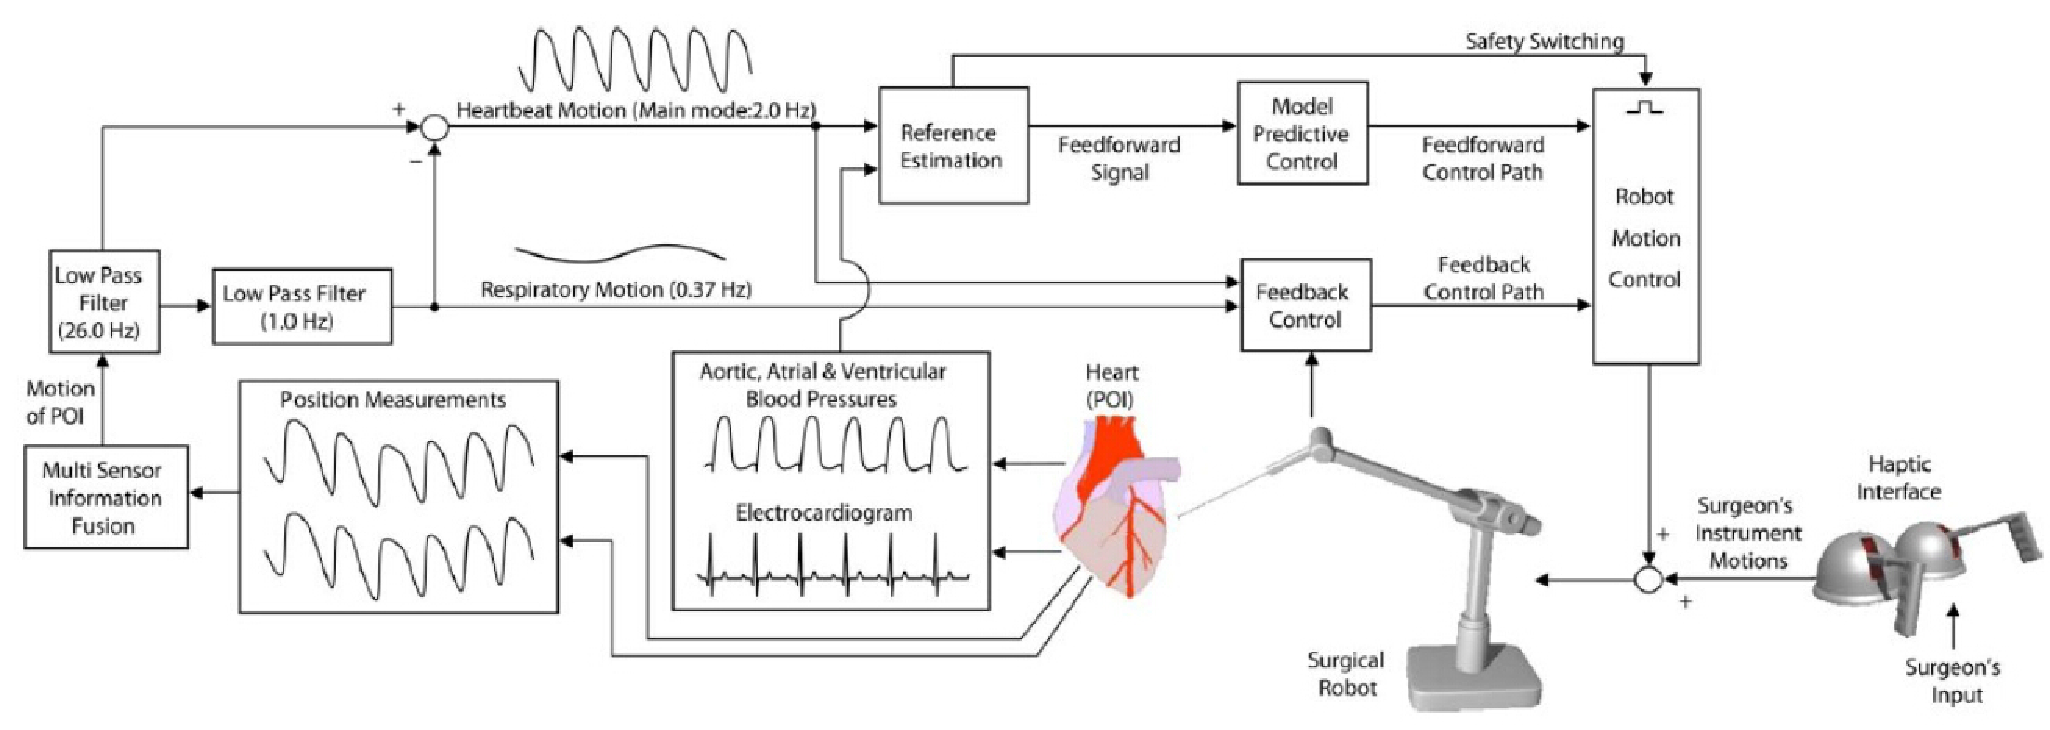
\includegraphics[width=\textwidth]{chapter5_BHR_control.pdf}
\caption{Control architecture for BHR}
\label{bhrcontrol}
\end{figure*}

The control architecture is shown in Figure \ref{bhrcontrol} \cite{Bebek2007, Tuna2013}. . In the figure, sensors collect the blood pressure and electrocardiogram directly from the heart. Then they send the data to multi-sensor information fusion, which combines all the information and estimates the reference trajectory. Finally, the robot motion control block will drive the robot by following the reference estimation.

\section{Software Architecture and Data Collection}\label{softwareframe}

\subsection{Software Architecture}
For SABiR, we build a software system on top of the low-level controller. When a user interacts with the robot, this is what they see.  This system has three components: a GUI, a task delegator, and a robot proxy. Figure~\ref{sabirsw} shows the information flow between these when the robot performs a high level insert/extract needle operation.

\begin{figure*}[!thpb]
\centering
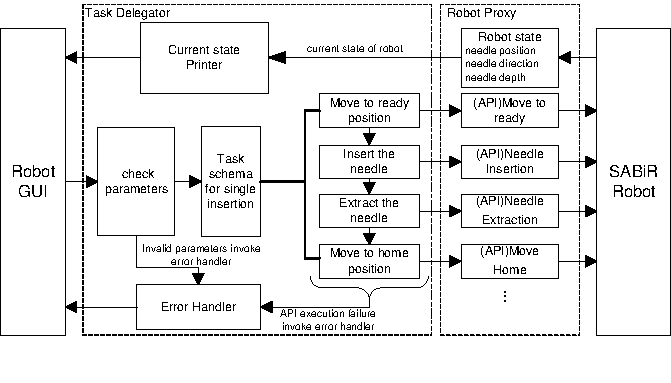
\includegraphics[width=\textwidth]{chapter5_SABiRsw.pdf}
\caption{Software Architecture of SABiR}
\label{sabirsw}
\end{figure*}

The software we build has a graphical user interface (GUI) that allows a user to view the current robot state and specify high level actions such as ``insert needle.'' For each such command, the GUI then lists all parameters whose values are needed to be input or adjusted. The data is then sent to a ``task delegator'' component. This first checks the validity of input parameters for the specified operation; for example, it ensures that target locations are within the robot's workspace. It then decomposes a complex task into a set of basic needle motions that can be accomplished by calls to the API for the robot (or the simulator). The delegator is equipped with different schemas to decompose different high level tasks. It then invokes the robot API to handle these decomposed tasks. As the task is being executed, it updates the robot's state on the GUI. If an error occurs, it is responsible for stopping the current action and alerting the user. The last stage, the ``robot proxy,'' handles communications with the robot (or simulation) and low-level operations and collects low-level sensor data from the robot (or simulation). This design ensures that when the simulation is replaced by the actual robot, only the last stage needs to be modified. Specifically, additional communication and synchronization code will be used to handle communications with the robot's controller (built on XPC) and to ensure that data collection between the software and hardware is properly logged.

\emph{1)}	Robot GUI: The robot GUI provides a graphical user interface through which user can view the robot state and issue commands to control the behavior of the robot. When user send a command to robot, the GUI will list all the parameters required by the command for user to input or adjust their values.

\emph{2)}	Task Delegator: The task delegator is the bridge between the robot and GUI.  If the user initiates a complex task, it is decomposed in the task delegator into a set of basic actions that can be accomplished by robot API calls. Take Figure \ref{sabirsw} as an example, when a single insertion is issued from the GUI, the task delegator does the following:

\emph{a)}	Collects and checks parameters: To make sure the user provided appropriate information for the specified task, the task delegator collects the parameters provided by the user and checks their validity . For a single insertion, the task delegator mainly check whether the insertion will reach the position out of the workspace of the surgery robot.

\emph{b)}	Decomposes the task and invokes robot API to perform the task:  If the parameters are valid, the task delegator and then decomposes the task into a set of basic actions and invokes the robot API to control the robot in performing the task. For task decomposition, the task delegator provides different kinds of schemas to dealing with different types of tasks. For example, a single insertion will be decomposed into four basic actions: move to ready position, insert the needle, extract the needle and move back to home position. Each basic action has an corresponding function in API, which can control the robot to accomplish the action.

\emph{c)}	Displays task status via the GUI: While the task is processing, the task delegator displays its current status and any error reports to the user via the GUI. For a single insertion, the task delegator continuously update the following information on the GUI: needle position, needle direction, the current time of the operation and which basic action the robot is doing. If any error happens during the task processing, the task delegator will stop the task and inform user through the GUI.

\emph{3)}	Robot Proxy: The robot proxy provides the robot API, which is a set of basic operations for controlling the robot and for checking its status. There is one version of the proxy for the actual robot and another for the robot simulator. Also, the active robot proxy records the state of the robot (e.g., its current needle position and direction).The basic operations includes robot initialization, move, insertion, extraction, move back to home position, stop robot,  reset robot parameter and etc.There is one version of the proxy for the actual robot and another for the robot simulator. To perform a specified basic operation, two API functions is involved. First, a function will be called to generate the reference trajectory of the operation. The reference trajectory will be temporally stored in robot proxy. Next, a function named \emph{runRobot} will be called to send the reference trajectory to the robot. Then the robot will move its needle to perform the operation by following the reference trajectory. Because reference trajectory generation algorithm is identical under different platforms, when the Robot's platform is changed (e.g., from simulator to actual robot), we only need to change the \emph{runRobot} function to fit the new platform.

For test purposes, the software system is used with the robot simulator. In the future, we will use it to control the actual robot. In our software framework, robot proxy is the only part to communicate with the robot(hardware). Thus, the robot GUI and task delegator will not change, but the robot proxy will be replaced by a new one which can talk to the actual robot. The robot proxy for actual robot provides the same API operations as the one for simulator. But the implementation of each robot API operation will change to fit the real robot platform. Specifically speaking, two robot proxy has different \emph{runRobot} functions.

\subsection{Data Collection}\label{subsec:datacollection}
We build the entire architecture to be easy to monitor and log. We base the data collection subsystem on the producer/consumer synchronization technique. We collect software execution data at the function level. That is, calling each function in the robot API
creates an object, which records the software state of the function's execution. This object is sent to a buffer queue through the producer. When the hardware data is available, the consumer thread starts to get the corresponding software state object from the queue and records both software data and hardware data in a user readable format. For example, when the robot begins to insert the needle, two software state objects are created and sent to the buffer queue. The first records the software states like action name ``insert'', depth of the needle inside tissue during the reference trajectory generation. The second records variables such as Motor Speed Error, which are estimated by the software after hardware data is available. Then another object is created to record only the hardware data of the action ``insert'' and sent to the buffer queue. When the consumer is not writing, it continuously takes objects out of the buffer queue and puts them into a local queue. When the consumer gets an object with only hardware data, it starts writing. While it is recording the data, the system can continuously transmit additional software data through the Producer as long as the buffer queue is not full.

\section{Dynamic Bayesian Networks}\label{secdbn}
Based on the collected data, we use Dynamic Bayesian Networks(DBNs) \cite{feng, fengthesisi} to model the time-evolution of the state space of the embedded control system. We use $S_t$ denotes a set of variables which characterized the state of control system at time $t$. DBNs are first order Markov model that represent the  probability of the next state given the current one, i.e $Pr(S_{t+1}|S_t)$. The factored stated transition distribution is defined by the equation:
\begin{equation}
\Pr ({S_{t + 1}}|{S_t}) = \Pr ({\pmb{V}_{t + 1}}|{\pmb{V}_t}) = \prod\limits_{i = 1}^n {\Pr (V_{t + 1}^i|{\pmb{V}_t})}  = \prod\limits_{i = 1}^n {\Pr (V_{t + 1}^i|\pmb{V}_t^{par(i)})} 
\end{equation}
where ${\pmb{V}_t} = \{ V_t^i\} $ denotes all the variables at time $t$. ${\pmb{V}_t^{par(i)}}$ denotes all the variables at time $t$ that have an effect to ${V_{t + 1}^i}$. Figure \ref{dbns} shows an example of DBN. Each node in the figure is associated with a conditional probability distribution (CPD), denoted as $\prod\limits_{i = 1}^n {\Pr (V_{t + 1}^i|\pmb{V}_t^{par(i)})} $, which is the probability distribution of $V^i$ given all the nodes in the previous time step that have an edge to it. From the equation above, the probability of the current state given the previous state equals the product of the CPD of each variable in the current state.
\begin{figure*}[!thpb]
\centering
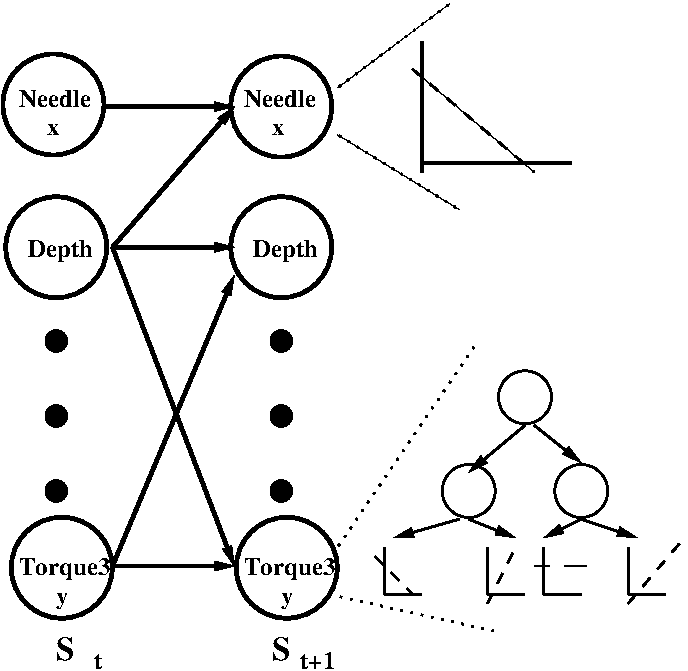
\includegraphics[width=0.6\textwidth]{chapter5_DBN}
\caption{Example Dynamic Bayesian Network}
\label{dbns}
\end{figure*}

To model CPDS, we applied two different models:{\it linear Gaussian model} and {\it regression tree model}. Because the robot controllers are designed to maintain a constant velocity in each high level action, we use {\it linear Gaussian model} to model some state variables which vary at a linear time rate from time $t$ to time $t+1$. For example, the variable represent $x$ axis of the needle tip position is one of those variable. For variables which have nonlinear variation from $t$ to $t+1$, we use a regression tree model for the CPB. In chapter 4, we have discussed the structure of regression tree model and mentioned that regression tree can model the nonlinear relationship between the predictors (input variables) and the response (target variables). In this work, we trained a DBN for each instrumented variable with the data from normal behavior of the robot control systems. The trained DBN will be used in identifying anomalous variables from the data of abnormal behavior of the robot control systems. For the detail of fitting the regression tree, please refer to our previous work \cite{}. In prior work, we have shown that this model and the training procedure yields very accurate models of normal hardware/software dynamics for the SABiR system. 

\section{Fault Localization Method}\label{dbnflalg}
In this chapter, the fault localization method is based on our previous work called FLECS, which is proposed by Liang and Ray at 2014 \cite{sescps}. FLECS is a fault localization method in embedded control software with Dynamic Bayesian Networks. It contains two steps: (1) identifying anomalous variables and (2) identifying faulty statements. In this research, we modified the algorithm of identifying faulty statements in FLECS. The modified method is named as FLECS 2.0. 

\subsection{Identifying anomalous variables}
In section \ref{secdbn}, we mentioned that the DBNs are trained with the data collected from normal behavior of the robot. Thus, given a set of input variables ${\pmb{V}_t}$ which represents abnormal behavior of the system at time $t$, the output of DBN $ {\pmb{{\hat V}}_{i + 1}} $ will be the predicted normal behavior of the system at time $t+1$ based on the input ${\pmb{V}_t} $. If the values of some variables in the predicted state $ {\pmb{{\hat V}}_{i + 1}} $ are significantly different from the corresponding values of variables in the observed state  $ {\pmb{V}_{i + 1}} $, we identified these variables as anomalous variables. The identification of anomalous variables contains three steps.

First, we need to label the data of anomalous trajectories. An anomalous trajectory contains more than 10 thousand data points and each data point represents the state of the robot at a specific time $t$. But not all the data points in anomalous trajectories are considered as {\it "failing"} runs, because the bugs in the control software may only influence part of the trajectory. Thus, it is important to {\it extract} the {\it "failing"} runs from the data of the whole trajectories as the input of DBNs. This step can be done automatically by checking if the observed end effector position at time $t$ is same as the reference end effector position at time $t$. But since the data of observed end effector position comes from the hardware sensors, there is always some error between observed position and referenced position due to the noise of hardware.  In experiment, we label a data point as {\it "failure"} when the difference between of observed end effector position and reference end effector position exceeds a pre-defined tolerance $\epsilon$. This is similar to labeling the {\it "failing"} runs of numerical software. We need to point out that if programs producing complex outputs, manual inspection may be required to label the data.

Second, when the observation of a variable is different from the prediction of DBN. we need to set a threshold to decide if this is an anomalous variable. To address this problem, we maintain a range of normal likelihoods of $\Pr ({\pmb{V}_{t + 1}}|{\pmb{V}_t})$, which we calculate from the training data that was used to train DBNs.  Given the training data, which are all normal data points, we go through each pair of points and calculate the negative log likelihood (NLL) for all the variables. The negative log likelihood for a state $S_{t+1}$ given its previous state ${S_t}$ is computed as follows:

\begin{equation}
NLL({S_{s + 1}}|{S_t}) = \sum\limits_{i \in \{ Pred\} } {\frac{{{{(v_i^{pred}(t + 1) - {v_i}(t + 1))}^2}}}{{Var(i)}}} 
\end{equation}

where $Pred$ is the set of indices of predictable variables in the DBN, $v_{i}^{pred}(t+1)$ is the predicted value for variable $i$ at time $t + 1$, $v_{i}^{(t + 1)}$ is the real observed value for variable i at time $t+ 1$. $Var(i)$ is the variance of the CPD (in our case either regression tree model or linear Gaussian model) over training data. Then we pick the highest NLL among all the normal data points as the threshold. 

Third, for all the variables in the data with {\it "fail"} label, we use DBNs to predict of the variable values at the next time step. The we calculate NLL for each variable. Whenever the variable?s NLL is larger than the threshold, we consider it to be an anomalous variable. Using this approach, we can pick a set of anomalous variables.

\subsection{Identifying faulty statements}
After we get a set of anomalous variables which are identified by the algorithm above, what we need next is to translate those variables into controller code to locate the faults. To do this,
we choose the controller?s dynamic PDG, which was induced by traversing the PDG from $S{t ?1}$, a normal input, to $S_t$ , an anomalous output. In our prior work FLECS, given a statement $s$, we sum the distances from the all statements containing the variables in the anomalous variable set as a total distance. The total distance is considered as the suspiciousness score of statement $s$. We rank the suspiciousness score and return a ranked list. But in this work, we proposed FLECS2.0, which modified method of calculating suspiciousness score of FLECS. 

\renewcommand{\algorithmicrequire}{\textbf{Input:}}
\renewcommand{\algorithmicensure}{\textbf{Output:}}
\begin{algorithm}
  \captionof{figure}{ {\it NUMFL} Algorithm}\label{flecs2.0}
  \begin{algorithmic}[1]
    \Require The software code of control system, simulator, trajectories with both normal and abnormal behavior
    \Ensure Ranked list of statements
    \State $D\leftarrow$ learned DBN from normal trajectories
    \State $T\leftarrow$ time index of start of anomalous event
    \State $t=T$; $BadVars\leftarrow \emptyset$; $WeightList\leftarrow \emptyset$; 
    \While  {$BadVars == \emptyset$ }
    	\State $BadVars\leftarrow$list of low-likelihoood variables at $t$ according to $D$
	\State $WeightList\leftarrow$list of weight of the variables in $BadVars$
	\State $t \leftarrow t+1$
    \EndWhile
    \State Sort $WeightList$ in descending order
    \State $P\leftarrow$ dynamic PDG of controller at $T$
    \State $O\leftarrow$ statements outputting $BadVars$ in $P$
    \State $Rank\leftarrow$ zero-element array of size number of nodes in $P$  
    \For  {$p$ a node in $P$ }
            \For  {$o$ a node in $O$ }
        		 \If{ p == o}
            		\State $Rank(p)=Rank(p)+30$
        		\ElsIf{$p$ is an ancestor of $o$}
			\State $d \leftarrow$ distance in $P$ from $p$ to $o$
			\State $r \leftarrow$ rank of the weight of $o$ in $WeightList$
            		\State $Rank(p)=Rank(p)+5/d+2/r$
        		\EndIf
   	    \EndFor
    \EndFor
    \Return statements in $P$ sorted by $Rank$
  \end{algorithmic}
\end{algorithm}


The algorithm of FLECS 2.0 is shown in Figure \ref{flecs2.0}. We first use DBN identified a set of anomalous variables $O$. Also, we assign a weight to each anomalous variable. The weight is equal to the difference between the NLL of the anomalous variable and the threshold. All the weights are stored in a list called weight list. Then given a statement $s$, we initialize its suspiciousness score as 0. We increase the suspiciousness score of $s$ in following two cases: (1) $s$ contains one or more variables in $O$. (2)$s$ contains a variable $p$ which is  the ancestor of a variable in $o \in O$ in PDG. The shorter the distance between $o$ and $p$ is, the more suspiciousness score $s$ received. The reason of increasing the suspiciousness score of $s$ in first case is straight forward. If $s$ is anomalous variable, we can infer that $s$ has erroneous state at $t+1$, which is possible to be the cause of the abnormal behavior of the system. For the second case, if $p$ is an ancestor of $o$, it means the value of $o$ is depend on the value of $p$ during the program execution. As a confounder, $p$ could be the cause of the abnormality of $o$ and thus $s$ should increase its suspiciousness score. 

We consider the first case is a stronger evidence that $s$ is faulty than the second case.  Assume the suspiciousness score of $s$ is increased by $m$ in the first case and is increased by $n$ in the second case, then we have $m>n$. The reason is that we have observed the abnormality of $s$ with the help of DBN in the first case. In the second case, the suspiciousness of $s$ comes from the fact that $p$ is a confounder of $o$,  but we did not observe the abnormality of $s$ from DBN.  Besides the above two cases, we also consider the weight of anomalous variables as a factor in suspiciousness score. If $p$ is an ancestor of $o$, we increase the suspiciousness score by a small value between 0 to $k$ according to the rank of the weight of $o$ in the weight list. The suspiciousness score increase more if the weight of $o$ has a higher rank in the list. In Figure \ref{flecs2.0}, we set $m=30$, $n=5$ and $k=2$. This is also the setting in our empirical evaluation.

Base on the algorithm in Figure \ref{flecs2.0}, we assigned a suspiciousness score to each statement in the control code. Then we sort all the suspiciousness scores in descending order. Once we get the sorted list, we can start debugging by tracing the statements all the way down from the top of the list. The debugging procedure is described as following steps: first we look at the first statement on the list. Then we localize it in the controller code and check if it is the bug that causes the anomalous event. If it is the buggy statement, we find the bug and fix it. If it is not the bug, we go to check the next statement in that list until we find the buggy statement.

\section{Empirical Evaluation}
We evaluate FLECS2.0 on the controllers of both SABiR and BHR. The controller of SABiR is written in MATLAB and has 330 lines of code in 6 functions, and contains 11 branches. We use the simulator we introduced in section \ref{secrobot} to generate both normal and abnormal trajectories of SABiR. The Normal trajectories are used to train DBNs and the abnormal trajectories are used to evaluate FLECS 2.0. The controller of BHR is also written in MATLAB and has 167 lines of code in 9 functions, and has no branches. We also trained DBNs for BHR with simulated trajectories. But for abnormal trajectories, we use the data collected from the hardware robot.

\subsection{Instrumenting the Controllers}
To collect data for our approach, we need to record the final values of variables after the controller finishes processing one time step. To keep the data collected reasonable, we chose to monitor 100 or fewer variables from each controller. We used two heuristics to determine which variables to monitor. First, for large matrices that are used in statements as a single entity (e.g. $X = A?B$), a candidate for monitoring is a single, randomly chosen element (from $X$ in this case). The rationale here is that if this statement is faulty, all the matrix elements are affected by it. However, if a statement uses a specific element from a matrix (e.g.$X(2, 2) = A(2, 3) ? B(3, 2)$) then that element is a candidate for us to monitor. For matrices of size ten or less, however, every entry was a possible candidate for monitoring.

We use a second rule to prune the list of candidates determined above. Here, we select those variables that are ?hub? variables in the controller?s PDG in that they influence many other variables? values. In our controllers, selecting variables that influence at least five other variables in the program gives us a reasonably sized set of variables to monitor. As a result of this selection process, we instrument 87 software variables from the controller of SABiR and 59 variables from the controller of BHR. The values of these variables are collected at every time step, after the controller finishes running, and used to generate training and testing data.

\subsection{Faulty Controllers}\label
To evaluate the techniques, we need buggy versions of the controllers. Through randomized testing we discovered one bug in the SABiR controller that triggers because of a missing check. This causes a subsequent square root computation to return a complex number of which only the real part is stored and processed, leading to anomalous behavior in the simulator. To generate additional bugs, we used mutation testing. Here we create a set of faulty versions of the controllers (mutants) through the randomized modification of elements of the code. This approach has been used in prior work \ref{}. We use four mutation operators: replace numerical constant, negate jump condition, change arithmetic operator, and add/subtract a small numeric value. We repeatedly randomly mutate an expression in the code and retain those which produce anomalous behavior. Through this process, we generated 10 faulty controllers for SABiR and 12 for BHR.

In the experiments, we use ESP-SCP and the original version of FLECS as baselines \ref{}.

\subsection{Methodology and Baselines}
We use 400 normal trajectories obtained through our simulator to train our DBN for SABiR and 10 trajectories to train a DBN for BHR. Each trajectory has 25,000 data points for SABiR and 11965 data points for BHR. For each trajectory generated with buggy versions of the SABiR controller that contained an anomalous event, we label the starting point manually by plotting the needle?s trajectory in MATLAB and comparing to the reference data. For BHR, we label points as anomalous using an automatic criterion, when the ?end effector error? variable goes beyond a predetermined normal threshold.

Each technique we use returns a ranked list of statements in the controller code. We report the rank of the first faulty statement in this list. In the case of ties, we place the faulty statement in the middle of the set of statements with the same score, which simulates a developer having to consider half of this list before finding the fault. The results of our experiments are shown in Table \ref{flbhr} and Table \ref{flsabir}.

Table \ref{flbhr} shows the result of experiments on BHR. FLECS 2.0 performs better than ESP-SCP on 9 faulty controller versions, but performs worse than ESP-SCP on 3 faulty controller versions.  FLECS 2.0 performs better than FLECS on 8 faulty controller versions, but performs worse than FLECS on 2 faulty controller versions. There are also two faulty version that FLECS and FLECS 2.0 have the same performance. Bug 6 is particularly interesting, because we found that the automatic starting point labeling criterion did not work well, and the labeled starting point was around 10000 steps before the true starting point of the anomalous event. Without the correction procedure described in section \ref{dbnflalg}, the faulty statement is ranked 134 by FLECS 2.0. The rank improves to 25 after the correction, indicating that this procedure can help correct for errors in the automatic labeling process. Table \ref{flsabir} shows the result of experiments on SABiR. FLECS 2.0 performs better than ESP-SCP on 8 faulty controller versions, but performs worse than ESP-SCP on 2 faulty controller versions.  FLECS 2.0 performs better than FLECS on 5 faulty controller versions, but performs worse than FLECS on 4 faulty controller versions. There is one faulty version that FLECS and FLECS 2.0 have the same performance. The first bug for SABiR in Table \ref{flsabir} is a real bug.  An interesting aspect of this bug is that the variables that were being computed by the faulty statements were not selected for monitoring in our list of 87 (for SABiR) variables that constitute the software state in our DBNs. However, some data dependencies of that statement were selected, and since this statement was the only fault in this experiment, it ?explained? many of these dependencies and so was ranked relatively highly. Overall, the experiment result shows that FLECS 2.0 outperforms ESP-SCP and original FLECS on two control system softwares. 

\begin{table*}[htbp!]
%\fontsize{10pt}{10pt}\selectfont
\centering
\caption{RANK OF THE FIRST FAULTY STATEMENT FOR BHR}
\label{flbhr}
      \begin{tabular}{|l|c|c|c|}
      \hline
Bug Index	&	ESP-SCP	&	FLECS	&	FLECS2.0	\\ \hline
1	&	85	&	73	&	15	\\ \hline
2	&	84	&	24	&	44	\\ \hline
3	&	60	&	97	&	18	\\ \hline
4	&	12	&	24	&	32	\\ \hline
5	&	13	&	14	&	9	\\ \hline
6	&	33	&	83	&	25	\\ \hline
7	&	81	&	61	&	12	\\ \hline
8	&	31	&	61	&	14	\\ \hline
9	&	11	&	14	&	56	\\ \hline
10	&	33	&	140	&	140  \\ \hline
11	&	81	&	90	&	22	\\ \hline
12	&	59	&	65	&	21	\\ \hline
\end{tabular}
\end{table*}

\begin{table*}[htbp!]
%\fontsize{10pt}{10pt}\selectfont
\centering
\caption{RANK OF THE FIRST FAULTY STATEMENT FOR SABiR}
\label{flsabir}
      \begin{tabular}{|l|c|c|c|}
      \hline
Bug Index	&	ESP-SCP	&	FLECS	&	FLECS2.0	\\ \hline
1	&	249	&	39	&	7	\\ \hline
2	&	1	&	3	&	26	\\ \hline
3	&	251	&	3	&	35	\\ \hline
4	&	42	&	2	&	36	\\ \hline
5	&	218	&	28	&	23	\\ \hline
6	&	10	&	27	&	21	\\ \hline
7	&	49	&	65	&	17	\\ \hline
8	&	6	&	23	&	5	\\ \hline
9	&	263	&	10	&	10	\\ \hline
10	&	39	&	3	&	13	\\ \hline
\end{tabular}
\end{table*}

\section{Related Work}
The work most closely related to ours involves using probabilistic models to identify bugs in programs. Liu et al. propose the SOBER method \cite{}, which builds a probabilistic model for program predicates. If the probability that a predicate P evaluates to true in passing runs is significantly different from the probability that P evaluates to true in failing runs, P is judged to be related to program failure. SOBER models control dependences but not data dependences. 

Some papers have focused on software testing for MATLAB/Simulink applications. Zhan et al \cite{} proposed a search based framework to generate test data for a Simulink model. He et al [40] use an improved mutation testing technique to reduce the cost of test data generation for Embedded Simulink. This work does not address the problem of fault localization, however.

Most related research on the safety of medical robotic systems in the literature primarily focus on design of intrinsically safe systems, e.g. [2], [41], [42], [43], [44]. A related approach in hybrid systems is parameter synthesis [45]. Here system parameters, such as joint limits, power levels, mass, etc. are designed in such a way as to produce good behavior and minimize or eliminate risk and/or the system is designed to fail in a safe manner and come to a controlled halt so that it can be removed and the procedure completed manually. This is typically achieved by using actuators with limited power and speed, current limiters, etc. These approaches do not consider the software development process, however, and do not attempt to address the problem of developing tools to aid the development of the controller.

Online fault detection and diagnosis is a very well studied problem in general robotics and other hybrid systems (e.g. [46], [47], [48]). A common approach is to use probabilistic sequence models to represent the system and to perform online inference to detect when the system is in a faulty state. These models also typically focus on modeling the hardware and devote attention to efficient inference algorithms to account for the online setting. Recent work on diagnosis has started to look at software as well [49], though at a coarse level.

\section{Conclusions}
Control software is widely used in many embedded systems including robots and vehicles. Given the often safety critical nature of such systems, it is valuable to design automated aids to developing them. The characteristics of such systems often make coverage-based fault localization techniques unsuitable. We have presented an alternative value-based approach that also attempts to exploit the availability of simulators for control systems. Experiments using two medical robot prototypes developed in our labs indicate the approach is promising. In future work, we plan to collect more empirical data on the performance of our technique, as well as explore causal inference techniques to improve the effectiveness of the technique.

\chapter{Conclusions and future work}\label{conclusion}
\section{Conclusions}
The dissertation focused on localizing faults in numerical softwares with causal inference technique.  The coverage based CSFL techniques are  

For the positivity violation problem in CSFL, we have proved that two types of violations of positivity: structural violations and random violations, do exist in Baah et al’s CSFL technique. We established that structural violations are not harmful, but random violations can distort suspiciousness scores.  We proposed a modification to the way suspiciousness scores are assigned with Baah et al.’s technique to address random violations.  Our empirical results show that it improves the performance of Baah et al.’s technique. We also presented a probabilistic characterization of Baah et al’s estimator which is more efficient way to compute the same scores. 

For the fault localization in numerical softwares, we proposed two models: NUMFL and BART.  In NUMFL model, we employs two different propensity scores, GPS and CBPS, to control confounding bias involving floating-point program variables that carry erroneous values to correct statements.  Then a quadratic regression model is used to estimate the AFCE of a numerical expression. The empirical results show that NUMFL is more effective than five well known SFL baseline techniques. Also GPS is more effective in controlling confounding bias comparing to CBPS. In BART model, we applied Bayesian additive regression trees to approximate the dose response function (DRF) of both the treatment variable and the confounding variables. Then we proposed a average causal effect estimation method based on BART for continuous treatment variable, which does not require techniques like propensity scores to control confounding bias. The empirical results show that BART is superior than NUMFL and other five baselines in fault localization of numerical software with single faults. In experiments, we found that the performance of BART is a robust to the training data size and the number of trees. We also discussed the computation time of NUMFL and BART. 

We extends our research to a special numerical software, embedded control systems, whose observational data is time series. We use dynamic Bayesian networks (DBNs) to model the time-evolution of the state space of the system. For fault localization, we improved our prior work and proposed FLECS 2.0. Our experiments use two medical robot prototypes developed in our lab. We developed a high-level software system to monitor the state of the robots and collect data for experiments. The empirical results show that the our technique is more effective than two baselines in localizing faults in embedded control systems.

\section{Future work}
In the future work, will seek to extend our empirical results to a broader range of subject programs with more varied fault types.  For NUMFL, we intend eventually to evaluate NUMFL in a user study, but given the difficulty of conducting an unbiased one, we think it is desirable to refine NUMFL as much as possible beforehand.  Finally, we will also explore the integration of NUMFL with coverage or predicate based causal SFL techniques. For BART model, we will seek to extend BART model to localize faults in non numerical softwares with statement coverage or predicate information. For FLECS 2.0, we plan to collect more empirical data on the performance of our technique, as well as explore causal inference techniques to improve the effectiveness of the technique. Also, if more embedded systems are available, we could test our technique on them. 












%-------------------------Appendix----------------------------------%
\appendix
\noappendicestocpagenum
\addappheadtotoc

 % Converted from Microsoft Word to LaTeX
% by Chikrii Softlab Word2TeX converter (version 5.0)
% Copyright (C) 1999-2011 Chikrii Softlab. All rights reserved.
% http://www.chikrii.com
% mailto: support@chikrii.com

% Warning: You are using Chikrii Softlab Word2TeX in TRIAL mode!
% In TRIAL mode some restrictions will apply.
% For more information please visit http://www.chikrii.com
% YOU CAN USE THIS FILE WITH THE SOLE PURPOSE OF EVALUATING Word2TeX.




\begin{appendices}
\chapter{Detail of the Derivation for Chapter 2}

\begin{equation}\label{ap:eq1}
\hat{\beta }_{1}=\frac{cov\left( \mathbf{c}_{s},\mathbf{c}_{s} \right)\bullet cov\left( \mathbf{t}_{s},\mathbf{y} \right)-cov\left( \mathbf{t}_{s},\mathbf{c}_{s} \right)\bullet cov\left( \mathbf{c}_{s},\mathbf{y} \right)}{cov\left( \mathbf{t}_{s},\mathbf{t}_{s} \right)\bullet cov\left( \mathbf{c}_{s},\mathbf{c}_{s} \right)-cov\left( \mathbf{t}_{s},\mathbf{c}_{s} \right)\bullet cov\left( \mathbf{t}_{s},\mathbf{c}_{s} \right)}
\end{equation}

We know that $cov\left( \mathbf{a},\mathbf{b}\right)=\frac{1}{n-1}\sum\nolimits_i {\left( a_{i}-\bar{a} \right)\left(
b_{i}-\bar{b} \right)} $. From equation above, $\hat{\beta }_{1}$ can be rewritten as:

\begin{equation}\label{ap:eq2}
\hat{\beta }_{1}=\frac{\sum\nolimits_i {\left( t_{s,i}-\bar{t_{s}}\right)\left( y_{i}-\bar{y} \right)\sum\nolimits_i \left(c_{s,i}-\bar{c_{s}} \right)^{2} -} \sum\nolimits_i {\left(c_{s,i}-\bar{c_{s}} \right)\left( y_{i}-\bar{y} \right)\sum\nolimits_i{\left( t_{s,i}-\bar{t_{s}} \right)\left( c_{s,i}-\bar{c_{s}} \right)} }}{\sum\nolimits_i {\left( t_{s,i}-\bar{t_{s}} \right)^{2}\sum\nolimits_i\left( c_{s,i}-\bar{c_{s}} \right)^{2} -} \left( \sum\nolimits_i {\left(t_{s,i}-\bar{t_{s}} \right)\left( c_{s,i}-\bar{c_{s}} \right)} \right)^{2}}
\end{equation}
Also, $\sum\nolimits_i {y_{i}=} n\bar{y}$ and $\sum\nolimits_i {t_{s,i}=}n\bar{t_{s}}$ , so we have:
\begin{equation}\label{ap:eq3}
\begin{aligned}
\sum\nolimits_i {\left( t_{s,i}-\bar{t_{s}} \right)\left( y_{i}-\bar{y} \right)} &=\sum\nolimits_i {t_{s,i}y_{i}-\bar{t_{s}}y_{i}-t_{s,i}\bar{y}+\bar{t_{s}}\bar{y}}\\
 &=\sum\nolimits_i {t_{s,i}y_{i}} -\sum\nolimits_i {\bar{t_{s}}y_{i}} -\sum\nolimits_i {t_{s,i}\bar{y}} +\sum\nolimits_i {\bar{t_{s}}\bar{y}}\\
  &=\sum\nolimits_i {t_{s,i}y_{i}} -n\bar{t_{s}}\bar{y}-n\bar{t_{s}}\bar{y}\mathrm{+}\, n\bar{t_{s}}\bar{y}\\
  &=\sum\nolimits_i {t_{s,i}y_{i}} -n\bar{t_{s}}\bar{y}
  \end{aligned}
\end{equation}
Similarly, we can derive the following equations:
\begin{equation}\label{ap:eq4}
\sum\nolimits_i {\left( c_{s,i}-\bar{c_{s}} \right)\left( y_{i}-\bar{y} \right)} =\sum\nolimits_i {c_{s,i}y_{i}} -n\bar{c_{s}}\bar{y}
\end{equation}

\begin{equation}\label{ap:eq5}
\sum\nolimits_i \left( c_{s,i}-\bar{c_{s}} \right)^{2} =\sum\nolimits_i c_{s,i}^{2} -n\bar{c_{s}}^{2}
\end{equation}

\begin{equation}\label{ap:eq6}
\sum\nolimits_i {\left( t_{s,i}-\bar{t_{s}} \right)\left( c_{s,i}-\bar{c_{s}} \right)} =\sum\nolimits_i {c_{s,i}t_{s,i}} -n\bar{c_{s}}\bar{t_{s}}
\end{equation}

\begin{equation}\label{ap:eq7}
\sum\nolimits_i \left( t_{s,i}-\bar{t_{s}} \right)^{2} =\sum\nolimits_i t_{s,i}^{2} -n\bar{t_{s}}^{2}
\end{equation}
With equation (3) - (6), we can rewrite the numerator of the quotient in
equation (2) as:
\begin{equation}\label{ap:eq8}
\begin{aligned}
numerator&=\left( \sum\nolimits_i {t_{s,i}y_{i}} -n\bar{t_{s}}\bar{y} \right)\left( \sum\nolimits_i c_{s,i}^{2} -n\bar{c_{s}}^{2} \right)\\
&-\left( \sum\nolimits_i {c_{s,i}y_{i}} -n\bar{c_{s}}\bar{y} \right)\left( \sum\nolimits_i {c_{s,i}t_{s,i}} -n\bar{c_{s}}\bar{t_{s}} \right)\\
&=\left( \sum\nolimits_i {t_{s,i}y_{i}} \sum\nolimits_i c_{s,i}^{2} -n\bar{t_{s}}\bar{y}\sum\nolimits_i c_{s,i}^{2} -n\bar{c_{s}}^{2}\sum\nolimits_i {t_{s,i}y_{i}}
+n^{2}\bar{t_{s}}\bar{y}\bar{c_{s}}^{2} \right)\\
&-\left( \sum\nolimits_i {c_{s,i}y_{i}} \sum\nolimits_i {c_{s,i}t_{s,i}} -n\bar{c_{s}}\bar{y}\sum\nolimits_i {c_{s,i}t_{s,i}} -n\bar{c_{s}}\bar{t_{s}}\sum\nolimits_i {c_{s,i}y_{i}} +n^{2}\bar{t_{s}}\bar{y}\bar{c_{s}}^{2} \right)
\end{aligned}
\end{equation}
We know that $\sum\nolimits_i c_{s,i}^{2} =n\bar{c_{s}}\mathrm{\, ,\,}\sum\nolimits_i c_{s,i}t_{s,i}=n\bar{t_{s}}$, so we have

\begin{equation}\label{ap:eq9}
\begin{aligned}
n\bar{t_{s}}\bar{y}\sum\nolimits_i c_{s,i}^{2} &=n^{2}\bar{t_{s}}\bar{y}\bar{c_{s}}\\
&=n\bar{c_{s}}\bar{y}\sum\nolimits_i {c_{s,i}t_{s,i}}
\end{aligned}
\end{equation}
Then equation(8) is equal to:
\begin{equation}\label{ap:eq10}
\begin{aligned}
numerator&=\sum\nolimits_i {t_{s,i}y_{i}} \sum\nolimits_i c_{s,i}^{2} -\sum\nolimits_i {c_{s,i}y_{i}} \sum\nolimits_i {c_{s,i}t_{s,i}} -n\bar{c_{s}}^{2}\sum\nolimits_i {t_{s,i}y_{i}} +n\bar{c_{s}}\bar{t_{s}}\sum\nolimits_i {c_{s,i}y_{i}}\\
 & ={(\mathbf{c}}_{s}\mathbf{\bullet }\mathbf{c}_{s}\mathbf{)(}\mathbf{t}_{s}\mathbf{\bullet y)}-(\mathbf{c}_{s}\mathbf{\bullet }\mathbf{t}_{s}\mathbf{)(}\mathbf{c}_{s}\mathbf{\bullet y)}-n\bar{c_{s}}^{2}\mathbf{(}\mathbf{t}_{s}\mathbf{\bullet y)+}n\bar{c_{s}}\bar{t_{s}}(\mathbf{c}_{s}\mathbf{\bullet y)}
 \end{aligned}
\end{equation}
Applying equation (5)-(7) to the denominator of the quotient in equation (2), we can rewrite it as:
\begin{equation}\label{ap:eq11}
\begin{array}{l}
denominator=\left( \sum\nolimits_i t_{s,i}^{2} -n\bar{t_{s}}^{2} \right)\left( \sum\nolimits_i c_{s,i}^{2} -n\bar{c_{s}}^{2} \right)-\left( \sum\nolimits_i {c_{s,i}t_{s,i}} -n\bar{c_{s}}\bar{t_{s}} \right)\left( \sum\nolimits_i {c_{s,i}t_{s,i}} -n\bar{c_{s}}\bar{t_{s}} \right)\\
=\left( \sum\nolimits_i t_{s,i}^{2} \sum\nolimits_i c_{s,i}^{2} -n\bar{t_{s}}^{2}\sum\nolimits_i c_{s,i}^{2} -n\bar{c_{s}}^{2}\sum\nolimits_i t_{s,i}^{2} +n^{2}\bar{t_{s}}^{2}\bar{c_{s}}^{2} \right)\\
-\left( \sum\nolimits_i {c_{s,i}t_{s,i}} \sum\nolimits_i {c_{s,i}t_{s,i}} -2n\bar{c_{s}}\bar{t_{s}}\sum\nolimits_i {c_{s,i}t_{s,i}} +n^{2}\bar{t_{s}}^{2}\bar{c_{s}}^{2} \right)\\
=\sum\nolimits_i t_{s,i}^{2} \sum\nolimits_i c_{s,i}^{2} -n\bar{t_{s}}^{2}\sum\nolimits_i c_{s,i}^{2} -n\bar{c_{s}}^{2}\sum\nolimits_i t_{s,i}^{2} -\left( \sum\nolimits_i {c_{s,i}t_{s,i}} \right)^{2}+2n\bar{c_{s}}\bar{t_{s}}\sum\nolimits_i {c_{s,i}t_{s,i}} \\
=\left( \mathbf{c}_{s}\bullet \mathbf{c}_{s} \right)\left( \mathbf{t}_{s}\bullet \mathbf{t}_{s} \right)-\left( \mathbf{c}_{s}\mathbf{\bullet }\mathbf{t}_{s} \right)^{2}-n\bar{t_{s}}^{2}\left( \mathbf{c}_{s}\bullet \mathbf{c}_{s} \right)\mathbf{-}n\bar{c_{s}}^{2}\left( \mathbf{t}_{s}\bullet \mathbf{t}_{s} \right)\mathbf{+}2n\bar{c_{s}}\bar{t_{s}}\mathbf{(}\mathbf{c}_{s}\mathbf{\bullet }\mathbf{t}_{s}\mathbf{)}
\end{array}
\end{equation}

\end{appendices}

\bibliographystyle{abbrv}
\bibliography{dissertation-BZF}

\end{document} 